\clearpage \newpage
\subsection{ EXPERIMENTOS}
%%CHICOS

%A280.TSP
\subsubsection{a280.TSP}
\begin{table}[hbtp]
 \centering
 \small
	\begin{tabular}{| l | l   l | r | r | r |   }
	    \hline\multicolumn{6}{|c|}{ \rowcolor[gray]{0.8}a280.TSP} \\\hline
     M  &\multicolumn{2}{|l|}{Resultado Original : 3418}   & Promedio & Mejor & Peor \\ \hline
        &                & Recocido  &  3364.17 & 3329 & 3394  \\ 
        & Con cuadrantes & Greedy    &  3363.79 & 3335 & 3396  \\ 
     X  &                & Genetico  &  3354.06 & 3318 & 3418  \\ \hline
     X  &                & Recocido  &  5078.51 & 4711 & 5345   \\ 
        & Sin cuadrantes & Greedy    &  5101.88 & 4804 & 5410   \\ 
        &                & Genetico  &  4876.34 & 4747 & 5066    \\ \hline
    \end{tabular}
    \caption{Experimento con la prueba a280.TSP}
    \label{table:EXP_a280.TSP}
\end{table}
 \begin{figure}[hbtp]
    \centering
        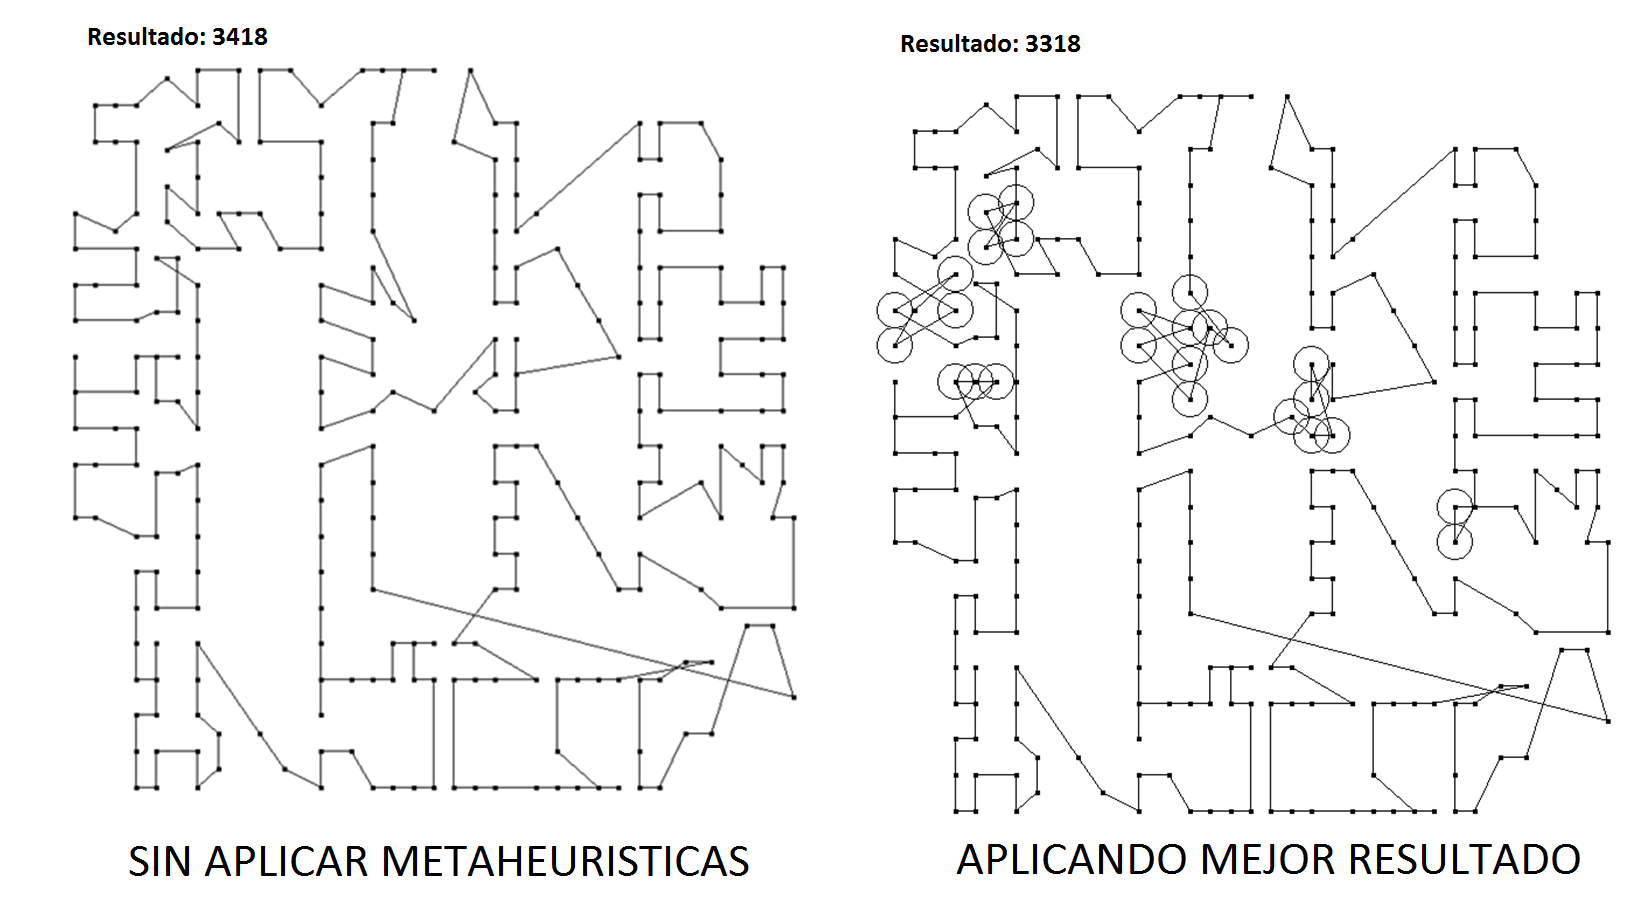
\includegraphics[width=1\textwidth]{PruebasResultados/Experimentos_Comparativas/a280.png}
        \caption{Comparativa a280.tsp}
        \label{fig:a280_comparativa.png}
\end{figure}
 \begin{figure}[hbtp]
    \centering
        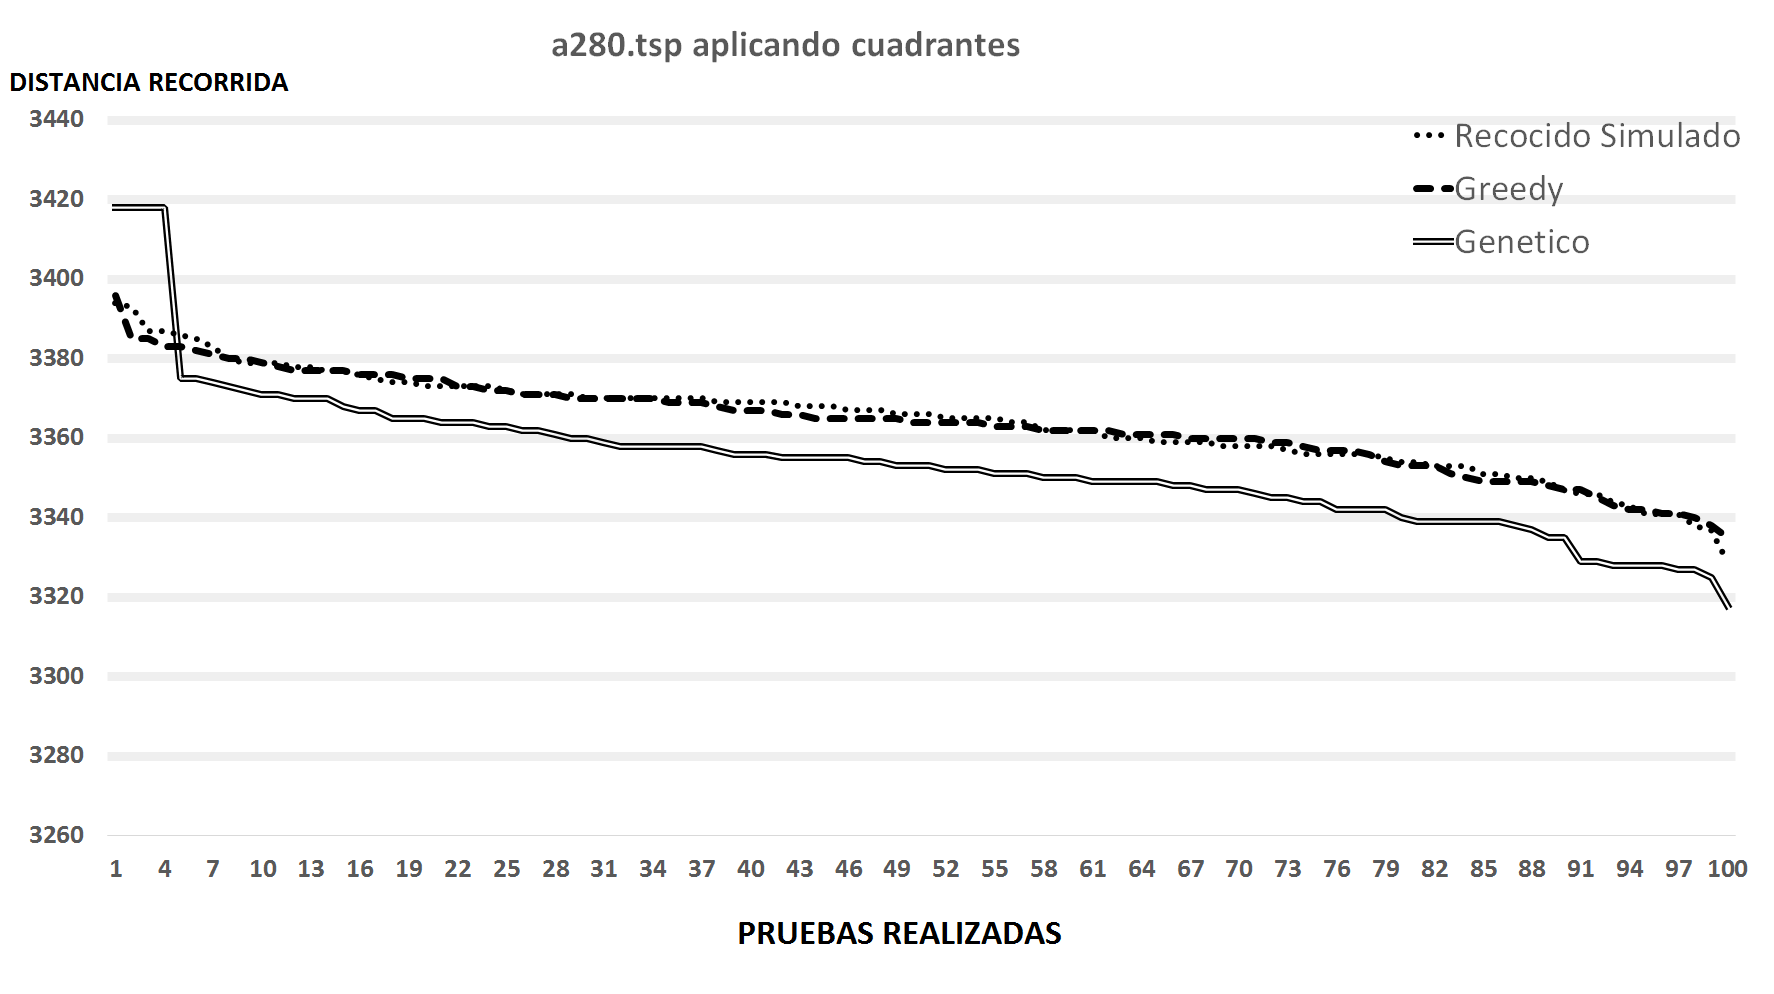
\includegraphics[width=0.9\textwidth]{PruebasResultados/Experimentos_Graficos_Con/a280.png}
        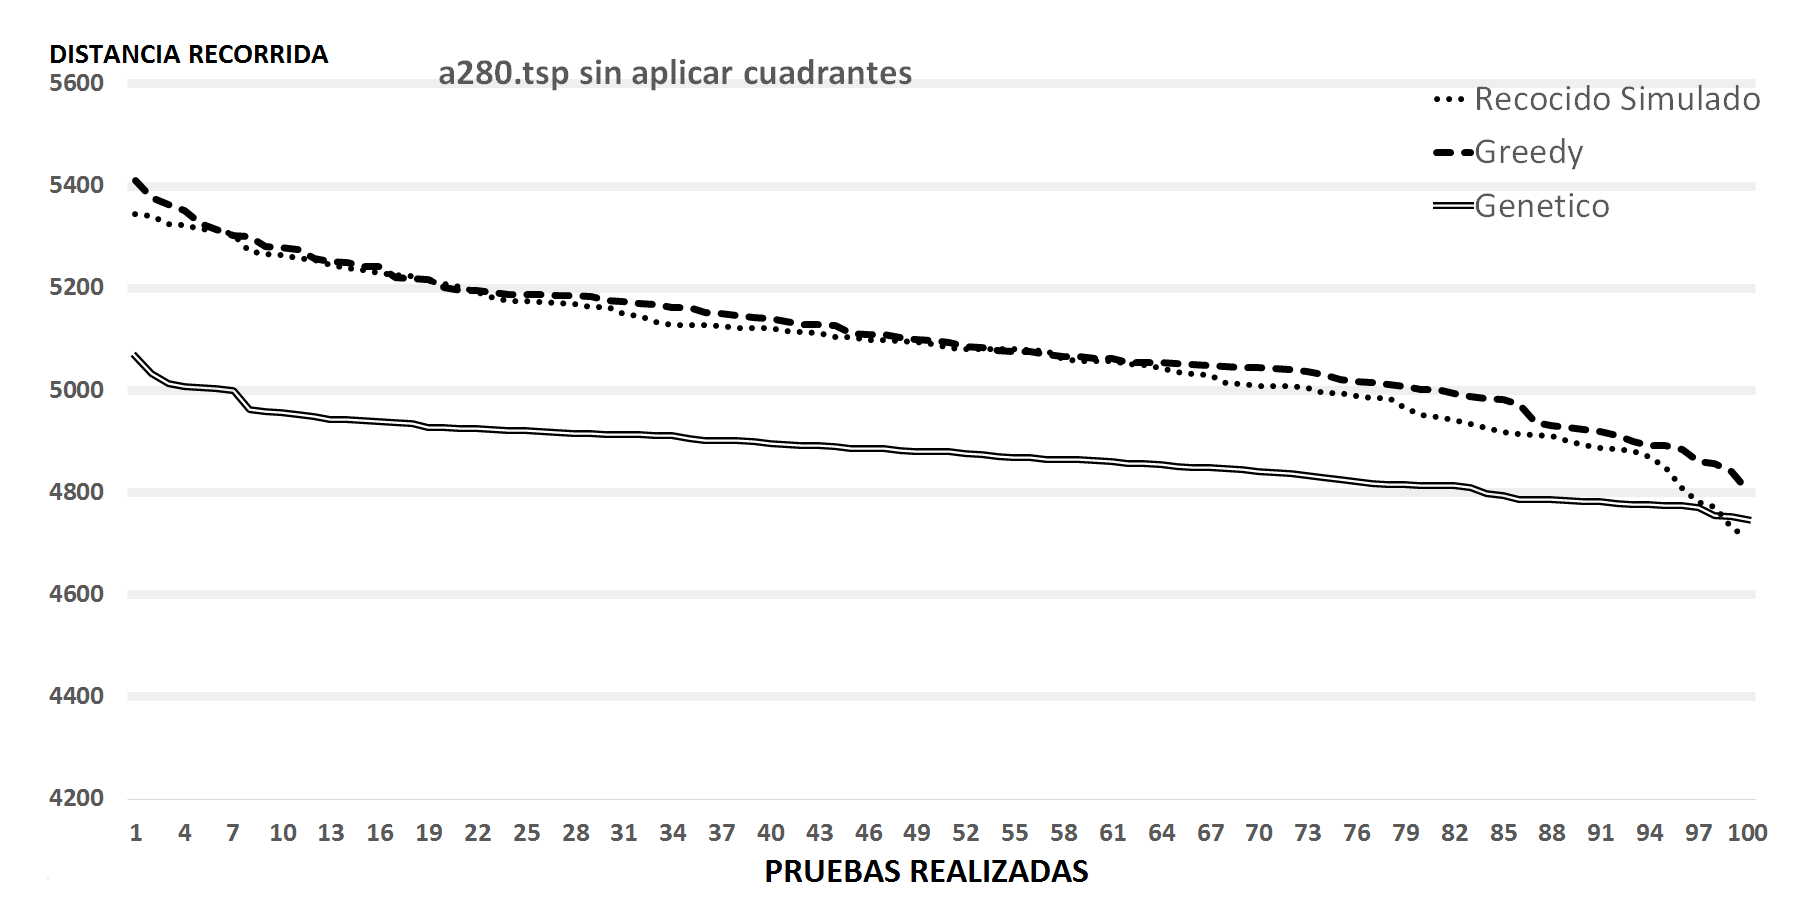
\includegraphics[width=0.9\textwidth]{PruebasResultados/Experimentos_Graficos_Sin/a280.png}
        \caption{Graficos a280.tsp con cuadrantes y sin cuadrantes}
        \label{fig:a280_grafica.png}
\end{figure}
\newpage

%CH150.TSP
\subsubsection{ch150.TSP}
\begin{table}[hbtp]
 \centering	
	\begin{tabular}{ | l   l | r | r | r |   }
         \hline\multicolumn{5}{|c|}{ \rowcolor[gray]{0.8} ch150.tsp } \\\hline
         \multicolumn{2}{|l|}{Resultado Original : 8579}   & Promedio & Mejor & Peor \\ \hline
                        & Recocido  &  8445.98 & 8272 & 8535  \\ 
         Con cuadrantes & Greedy    &  8446.02 & 8315 & 8540  \\ 
                        & Genetico  &  8358.81 & 8231 & 8427  \\ \hline
                        & Recocido  &  26500.85 & 23162 & 28674   \\ 
         Sin cuadrantes & Greedy    &  26614.55 & 22417 & 29187   \\ 
                        & Genetico  &  34548.11 & 32091 & 37844    \\ \hline
    \end{tabular}
    \caption{Experimento con la prueba ch150.tsp}
    \label{table:EXP_ch150.tsp}
\end{table}
 \begin{figure}[hbtp]
    \centering
        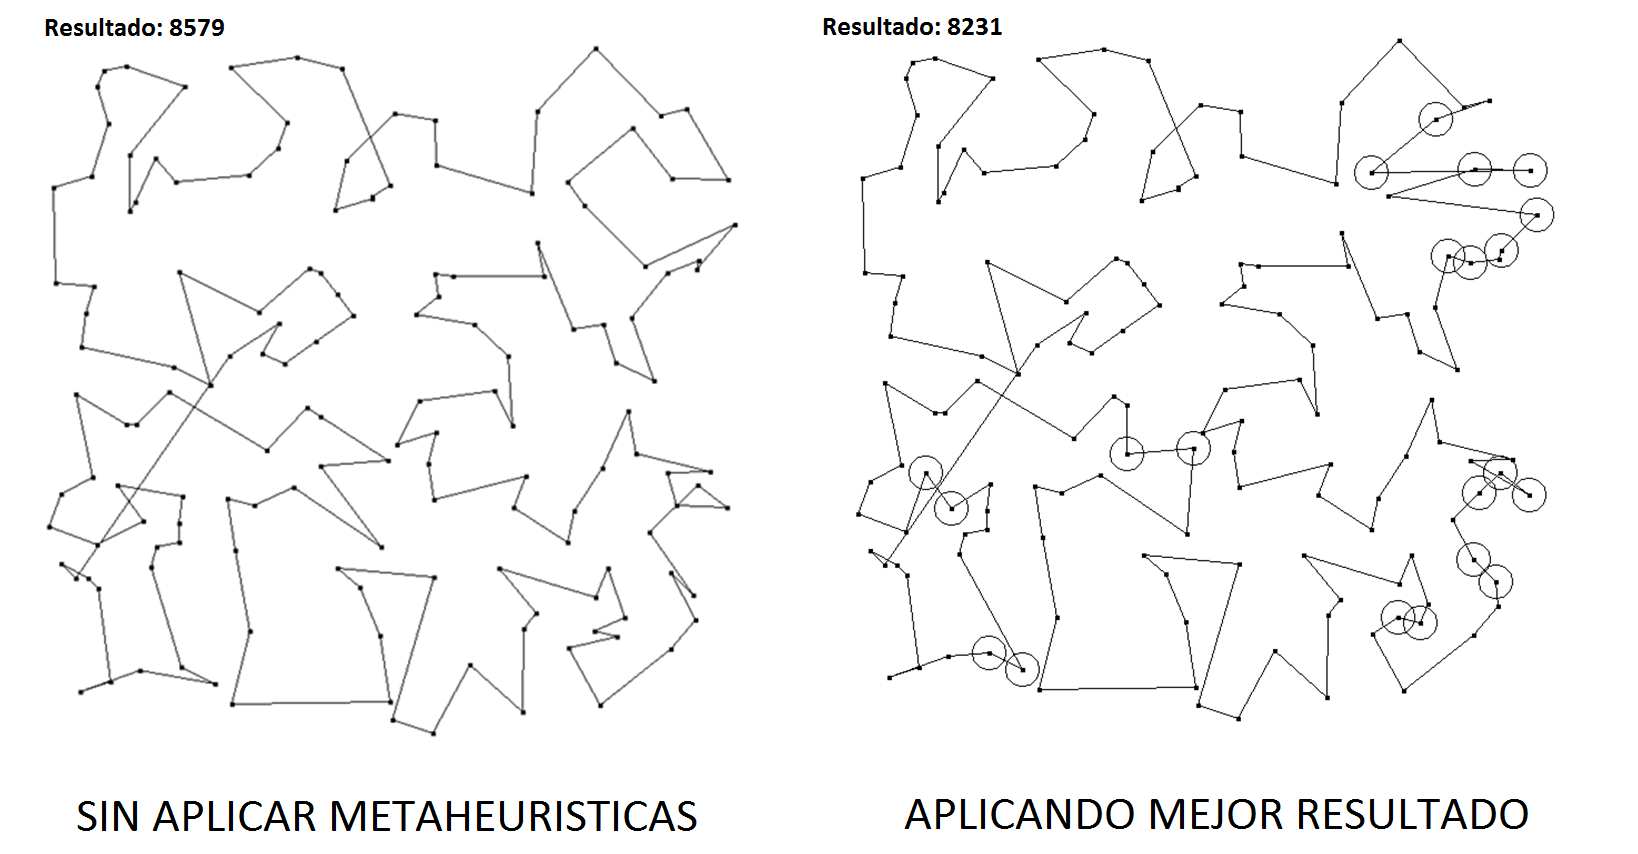
\includegraphics[width=1\textwidth]{PruebasResultados/Experimentos_Comparativas/ch150.png}
        \caption{Comparativa ch150.tsp}
        \label{fig:ch150_comparativa.png}
\end{figure}
 \begin{figure}[hbtp]
    \centering
        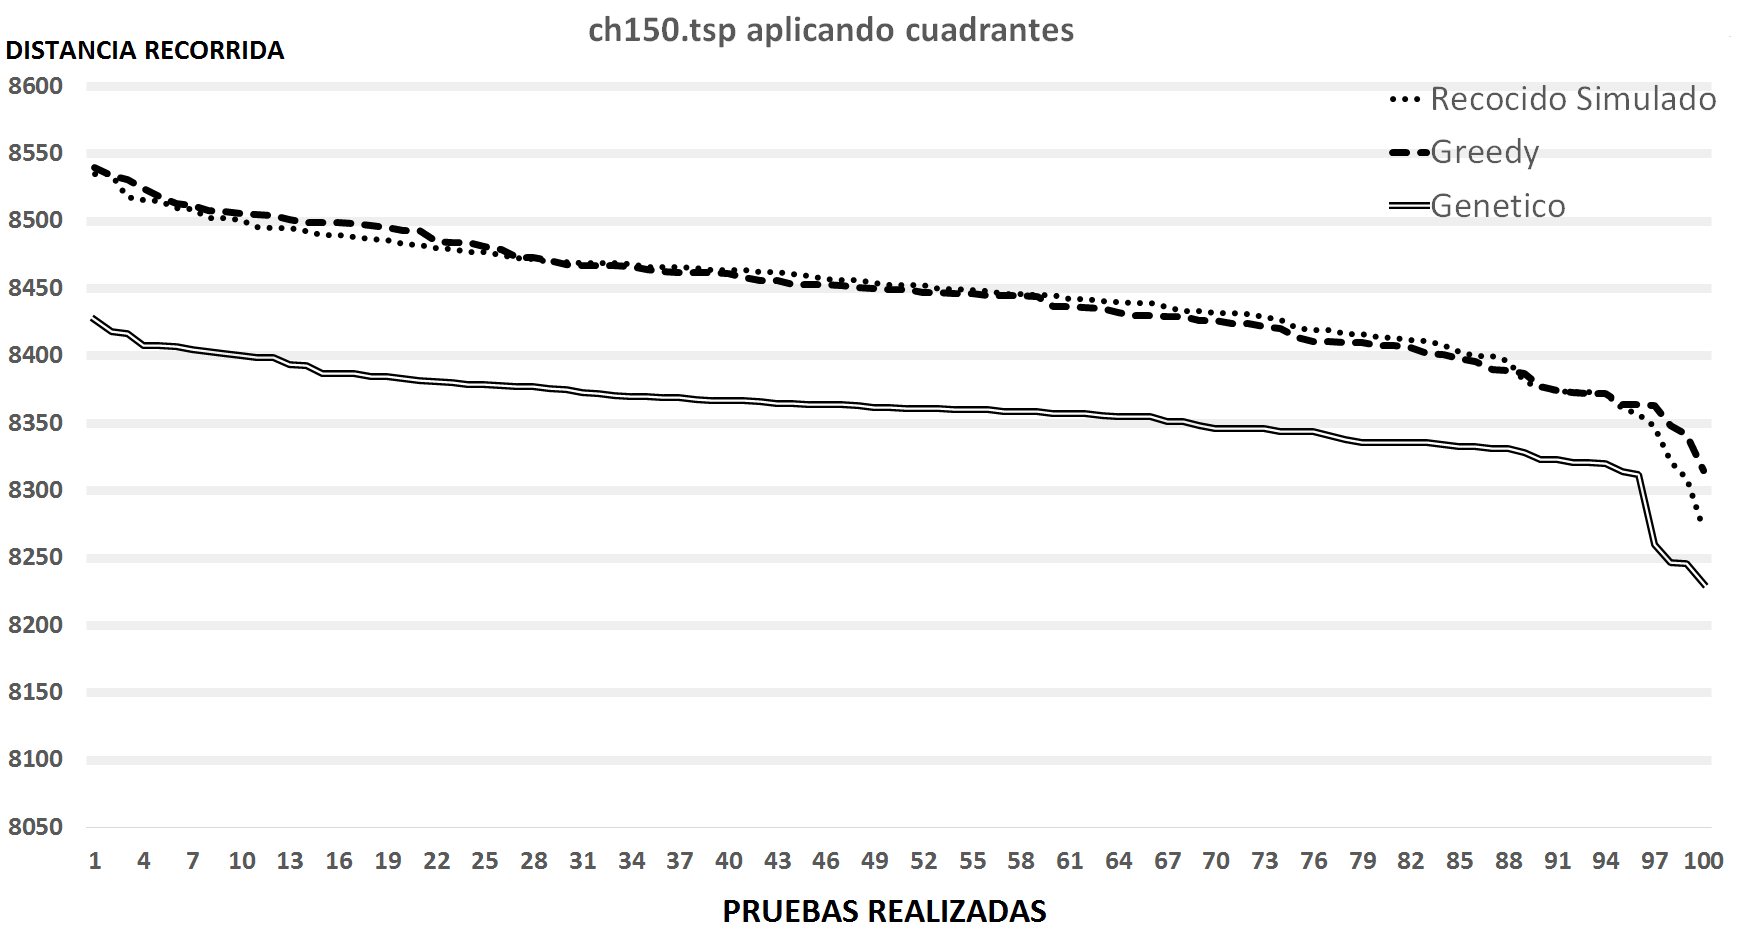
\includegraphics[width=0.9\textwidth]{PruebasResultados/Experimentos_Graficos_Con/ch150.png}
        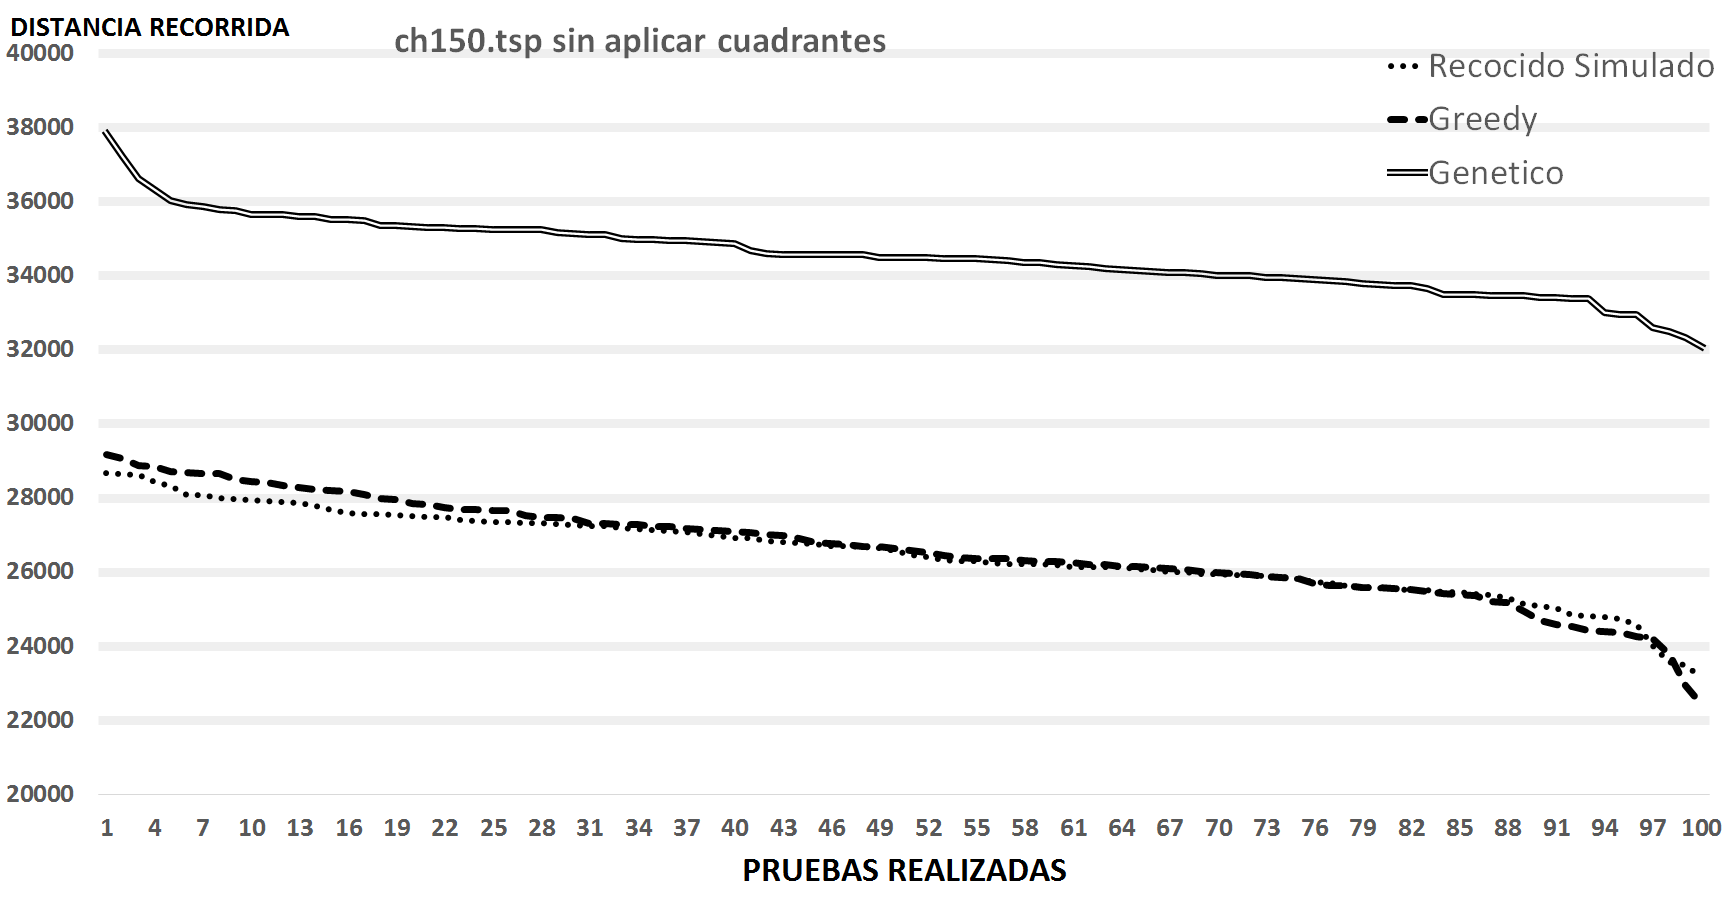
\includegraphics[width=0.9\textwidth]{PruebasResultados/Experimentos_Graficos_Sin/ch150.png}
        \caption{Graficos ch150.tsp con cuadrantes y sin cuadrantes}
        \label{fig:a280_grafica.png}
\end{figure}
\newpage

%EIL101.TSP
\subsubsection{eil101.TSP}
\begin{table}[hbtp]
 \centering
\begin{tabular}{ | l   l | r | r | r |   }
	    \hline\multicolumn{5}{|c|}{ \rowcolor[gray]{0.8}eil101.tsp} \\\hline
         \multicolumn{2}{|l|}{Resultado Original : 828}   & Promedio & Mejor & Peor \\ \hline
                        & Recocido  & 804.91 & 788 & 822  \\ 
         Con cuadrantes & Greedy    & 806.93 & 788 & 825  \\ 
                        & Genetico  & 787.33 & 781 & 802  \\ \hline
                        & Recocido  & 1747.41 & 1585 & 1917   \\ 
         Sin cuadrantes & Greedy    & 1744.97 & 1630 & 1855   \\ 
                        & Genetico  & 1705.49 & 1602 & 1740    \\ \hline
    \end{tabular}
    \caption{Experimento con la prueba eil101.tsp}
    \label{table:EXP_eil101.tsp}
\end{table}
 \begin{figure}[hbtp]
    \centering
        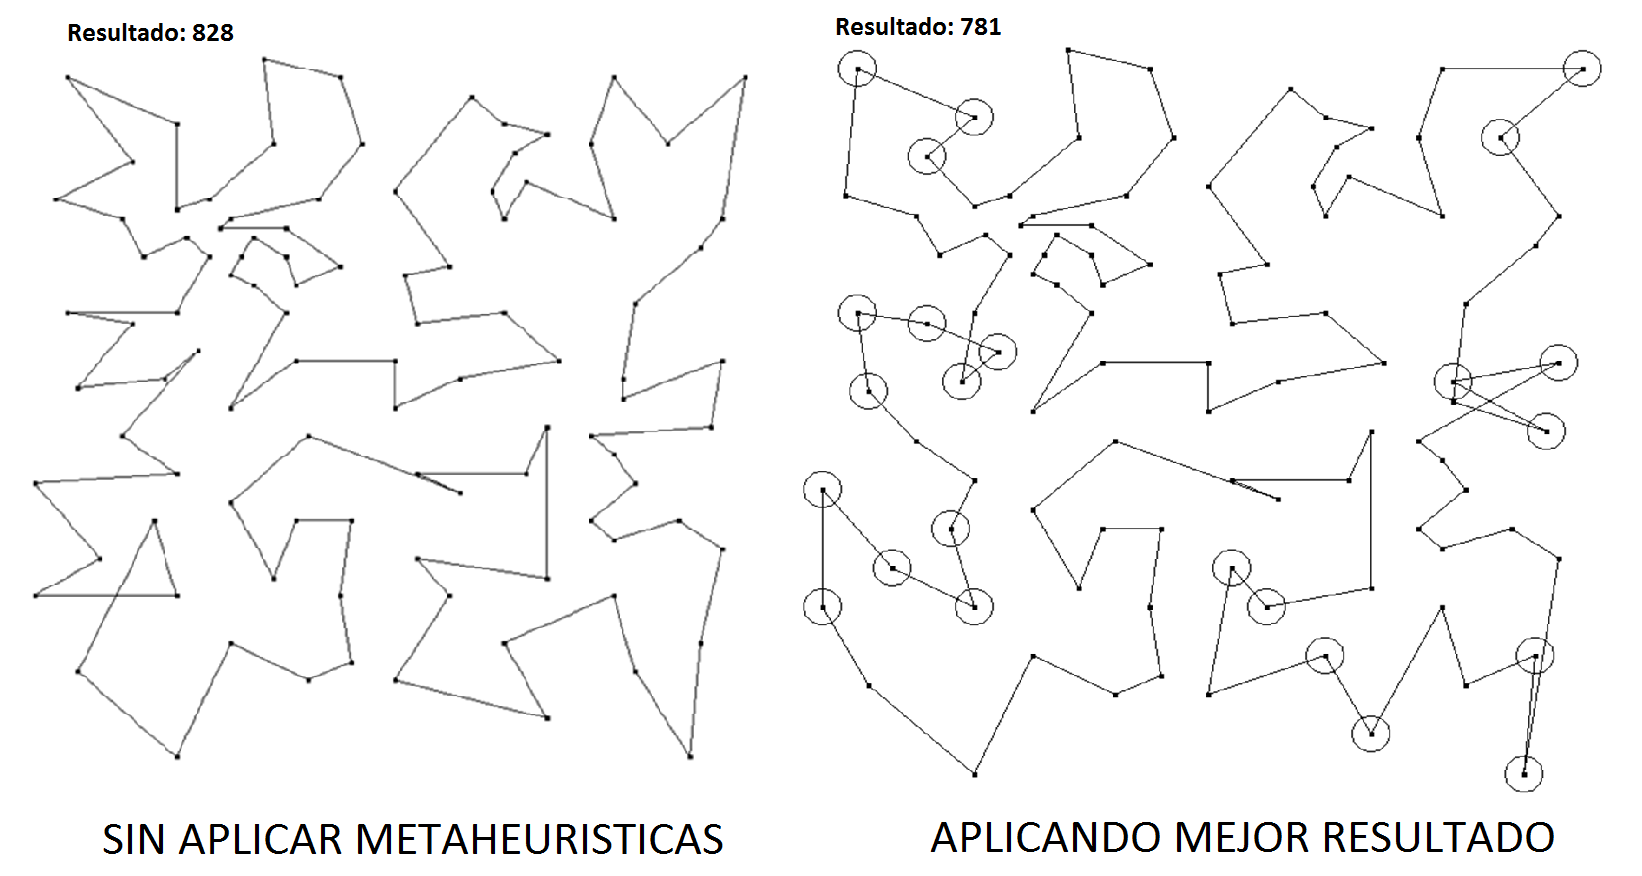
\includegraphics[width=1\textwidth]{PruebasResultados/Experimentos_Comparativas/eil101.png}
        \caption{Comparativa eil101.tsp}
        \label{fig:eil101_comparativa.png}
\end{figure}
 \begin{figure}[hbtp]
    \centering
        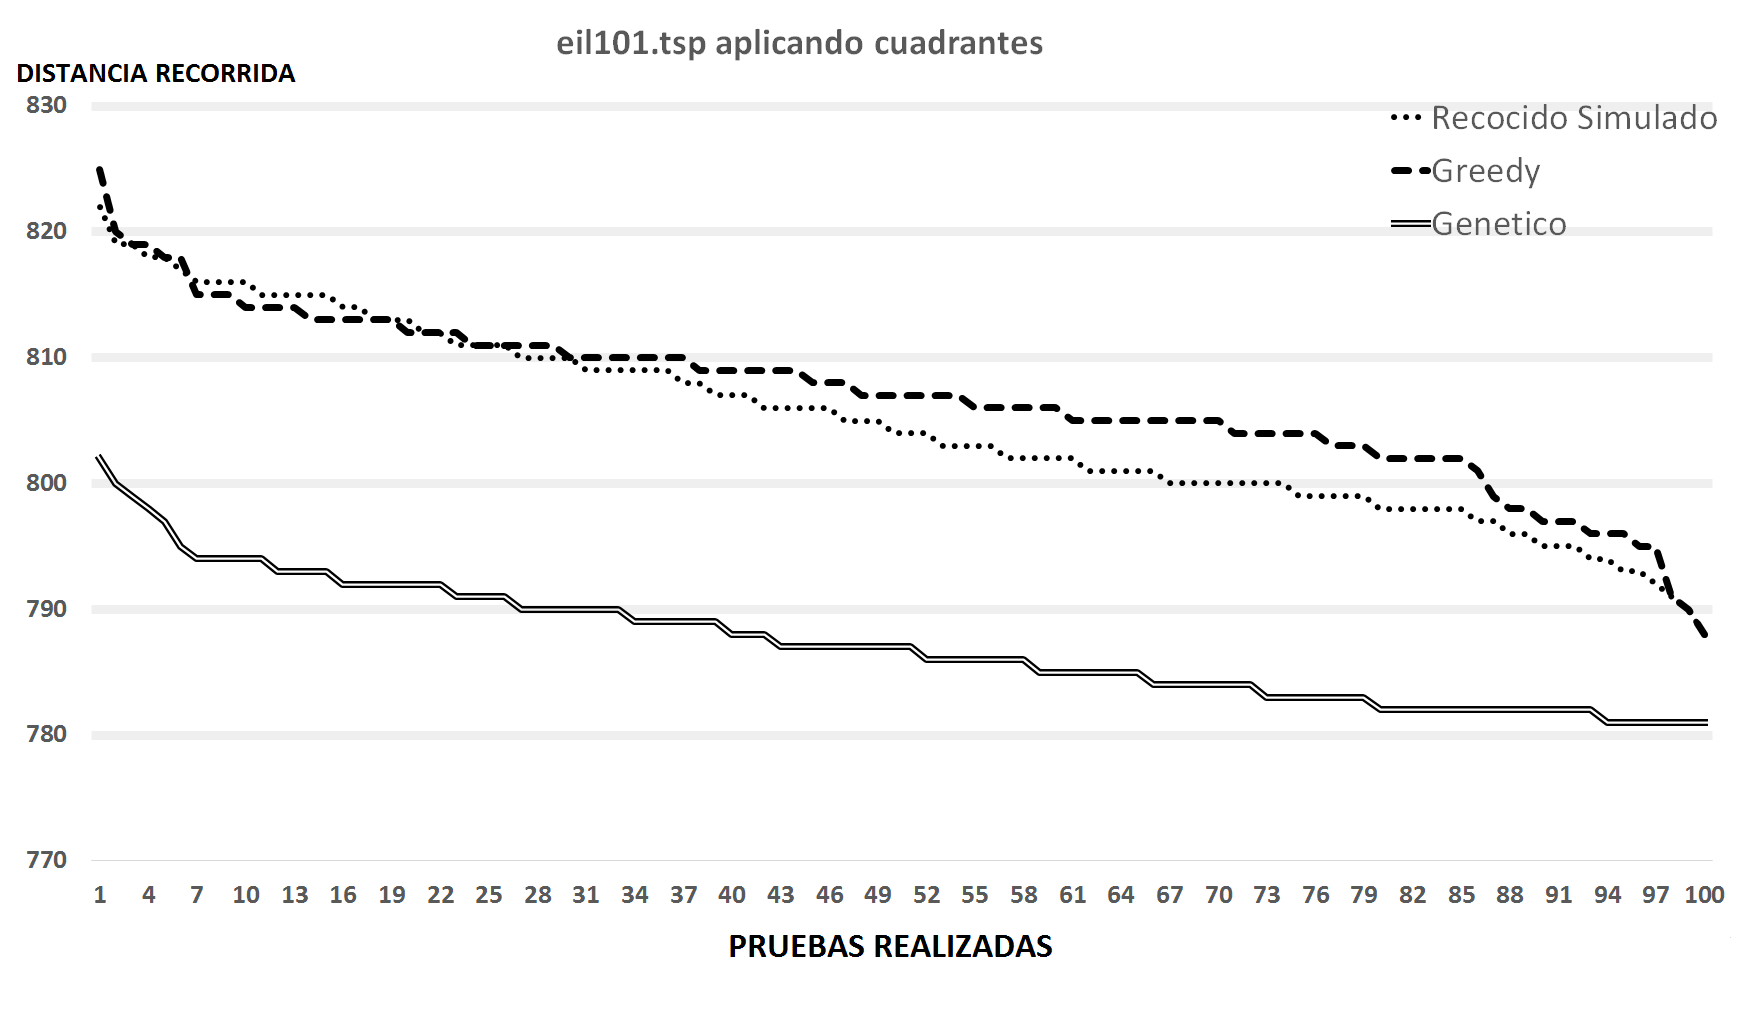
\includegraphics[width=0.9\textwidth]{PruebasResultados/Experimentos_Graficos_Con/eil101.png}
        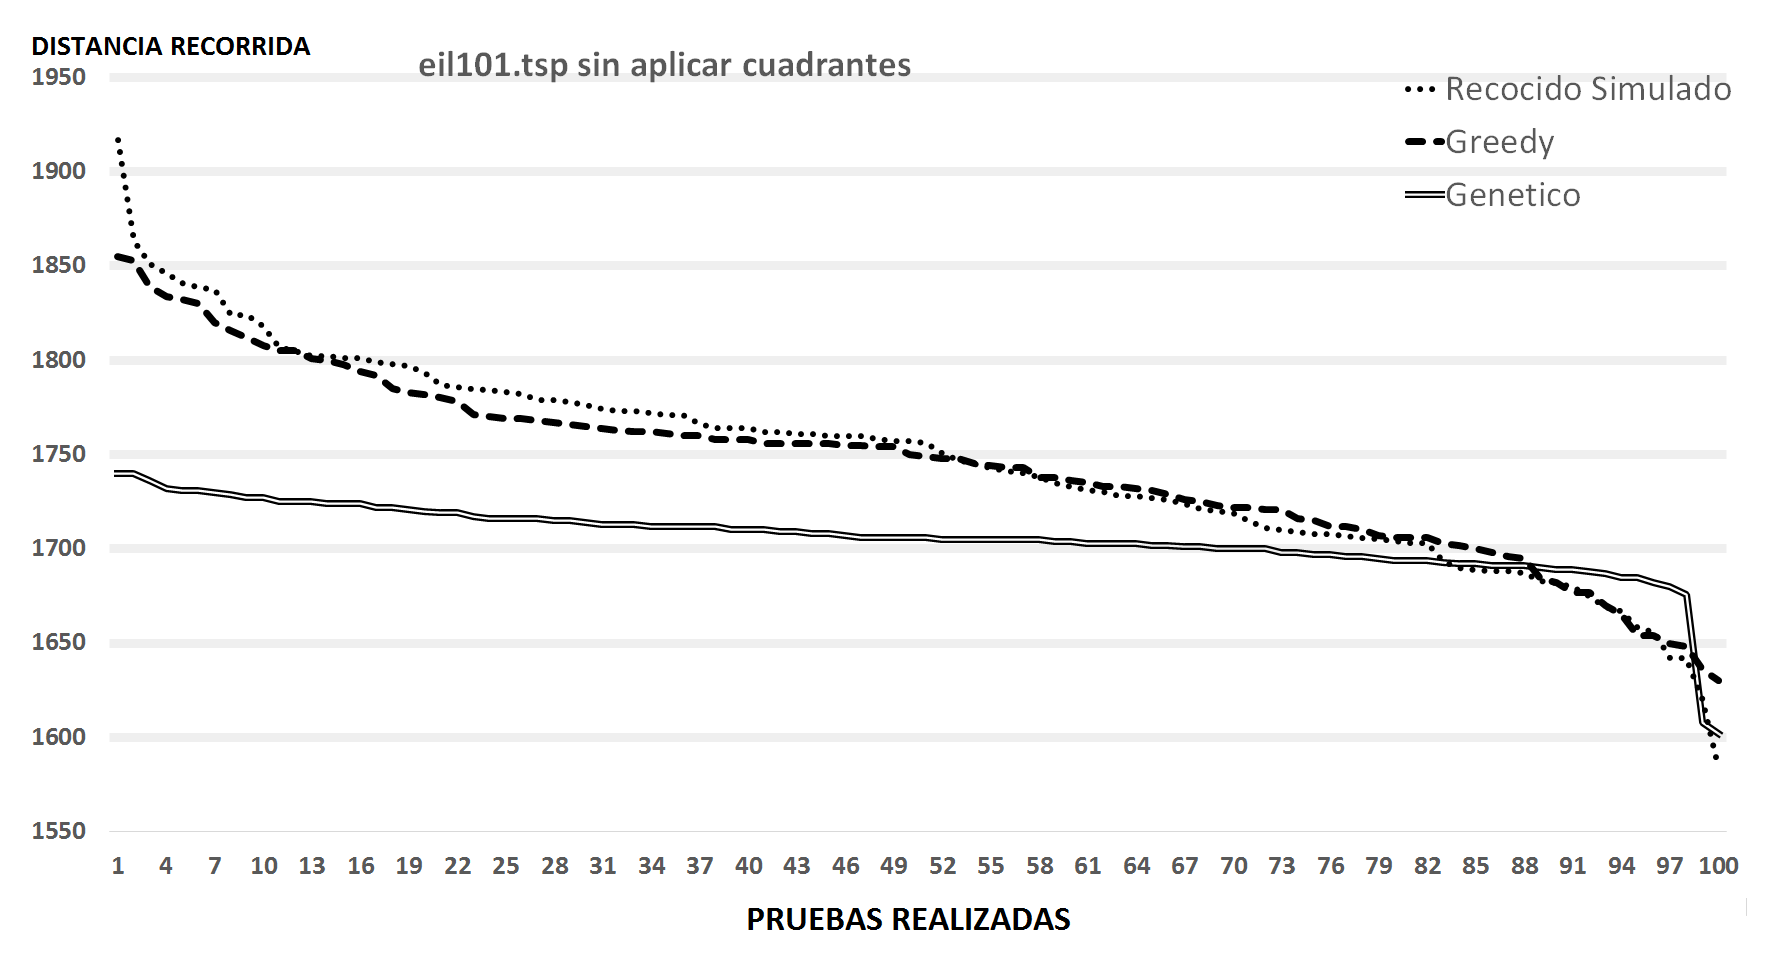
\includegraphics[width=0.9\textwidth]{PruebasResultados/Experimentos_Graficos_Sin/eil101.png}
        \caption{Graficos eil101.tsp con cuadrantes y sin cuadrantes}
        \label{fig:eil101_grafica.png}
\end{figure}
\newpage

%LIN318.TSP
\subsubsection{lin318.TSP}
\begin{table}[hbtp]
 \centering
	\begin{tabular}{ | l   l | r | r | r |   }
     \hline\multicolumn{5}{|c|}{ \rowcolor[gray]{0.8}lin318.tsp} \\\hline
     \multicolumn{2}{|l|}{Resultado Original : 55340} & Promedio & Mejor & Peor \\ \hline
                        & Recocido  & 54438.22 & 53752 & 55085  \\ 
         Con cuadrantes & Greedy    & 54367.97 & 53773 & 55073  \\ 
                        & Genetico  & 53997.96 & 53479 & 54344  \\ \hline
                        & Recocido  & 110739.67 & 102042 & 118920   \\ 
         Sin cuadrantes & Greedy    & 110691.43 & 104454 & 117441   \\ 
                        & Genetico  & 120441.11 & 114461 & 125074    \\ \hline
    \end{tabular}
    \caption{Experimento con la prueba lin318.tsp}
    \label{table:EXP_lin318.tsp}
\end{table}
 \begin{figure}[hbtp]
    \centering
        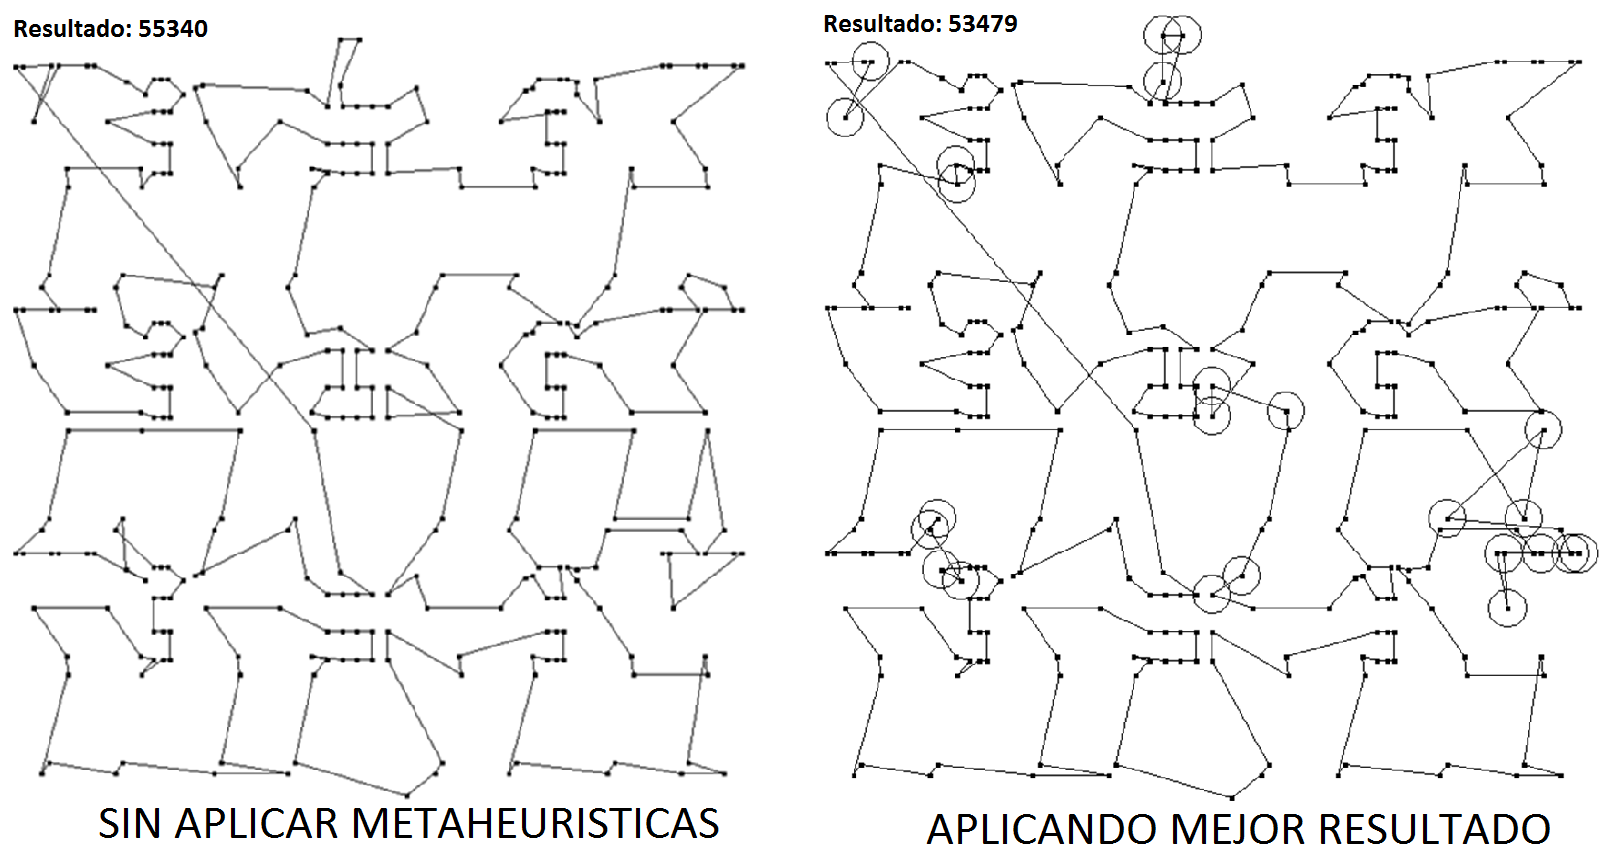
\includegraphics[width=1\textwidth]{PruebasResultados/Experimentos_Comparativas/lin318.png}
        \caption{Comparativa lin318.tsp}
        \label{fig:lin318_comparativa.png}
\end{figure}
 \begin{figure}[hbtp]
    \centering
        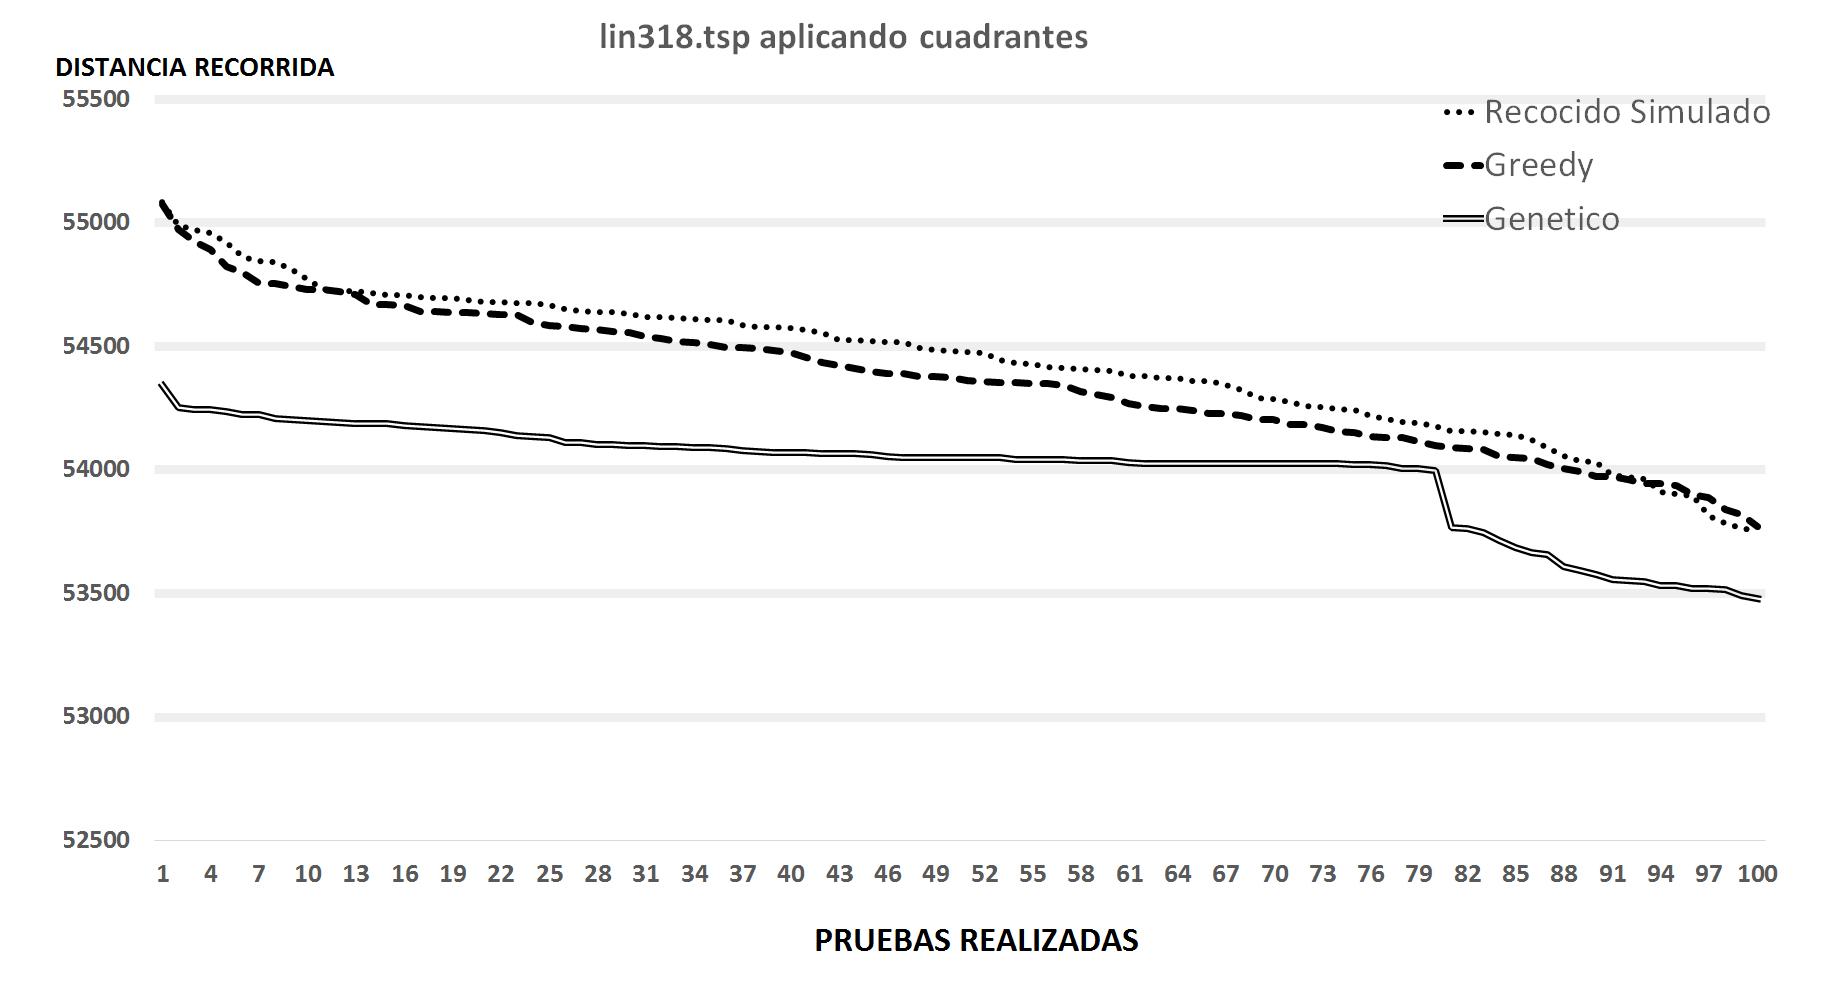
\includegraphics[width=0.9\textwidth]{PruebasResultados/Experimentos_Graficos_Con/lin318.png}
        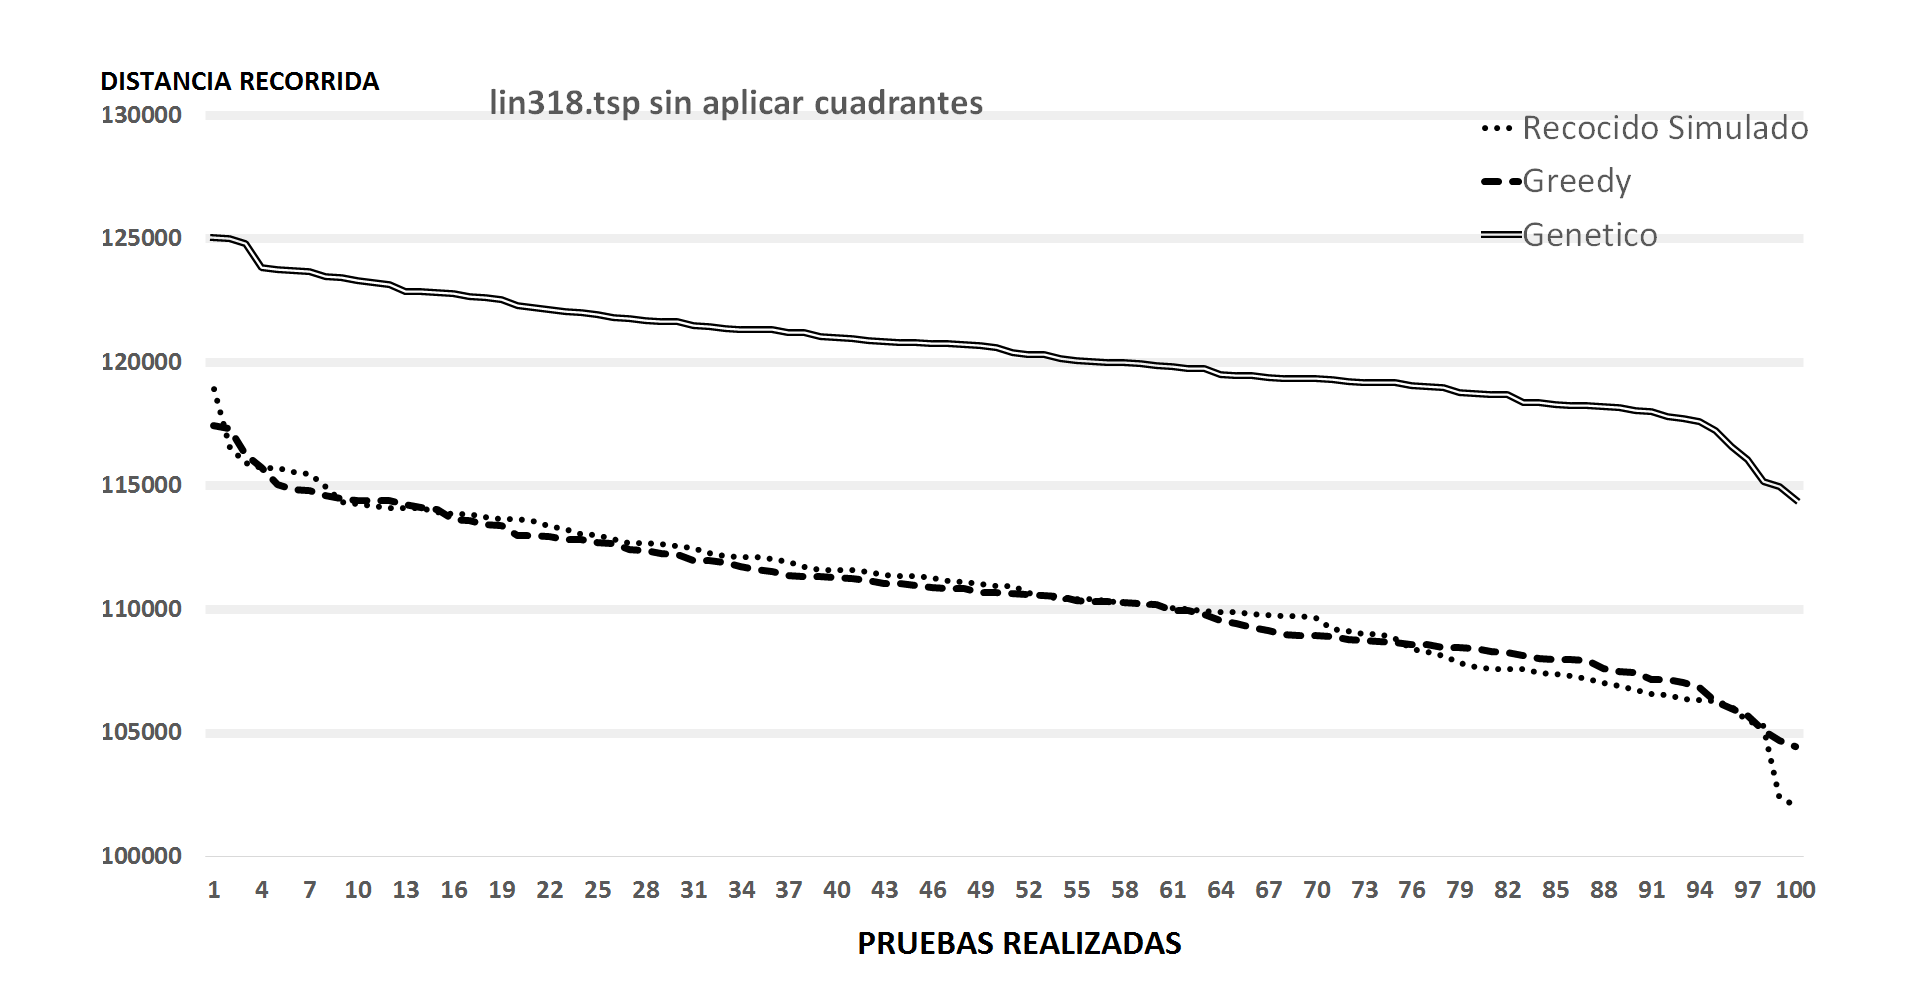
\includegraphics[width=0.9\textwidth]{PruebasResultados/Experimentos_Graficos_Sin/lin318.png}
        \caption{Graficos lin318.tsp con cuadrantes y sin cuadrantes}
        \label{fig:lin318_grafica.png}
\end{figure}
\newpage

%U159.TSP
\subsubsection{u159.TSP}
\begin{table}[hbtp]
 \centering 
	\begin{tabular}{ | l   l | r | r | r |   }
       \hline\multicolumn{5}{|c|}{ \rowcolor[gray]{0.8}u159.tsp} \\\hline
         \multicolumn{2}{|l|}{Resultado Original : 56495} & Promedio & Mejor & Peor \\ \hline
                        & Recocido  & 55506.95 & 54737 & 56021  \\ 
         Con cuadrantes & Greedy    & 55525.77 & 54992 & 56004  \\ 
                        & Genetico  & 54834.24 & 54418 & 55238  \\ \hline
                        & Recocido  & 68629.83 & 65324 & 74869   \\ 
         Sin cuadrantes & Greedy    & 68829.22 & 65058 & 73971   \\ 
                        & Genetico  & 62582.97 & 59906 & 65035    \\ \hline
    \end{tabular}
    \caption{Experimento con la prueba u159.tsp}
    \label{table:EXP_u159.tsp}
\end{table}
\begin{figure}[hbtp]
    \centering
        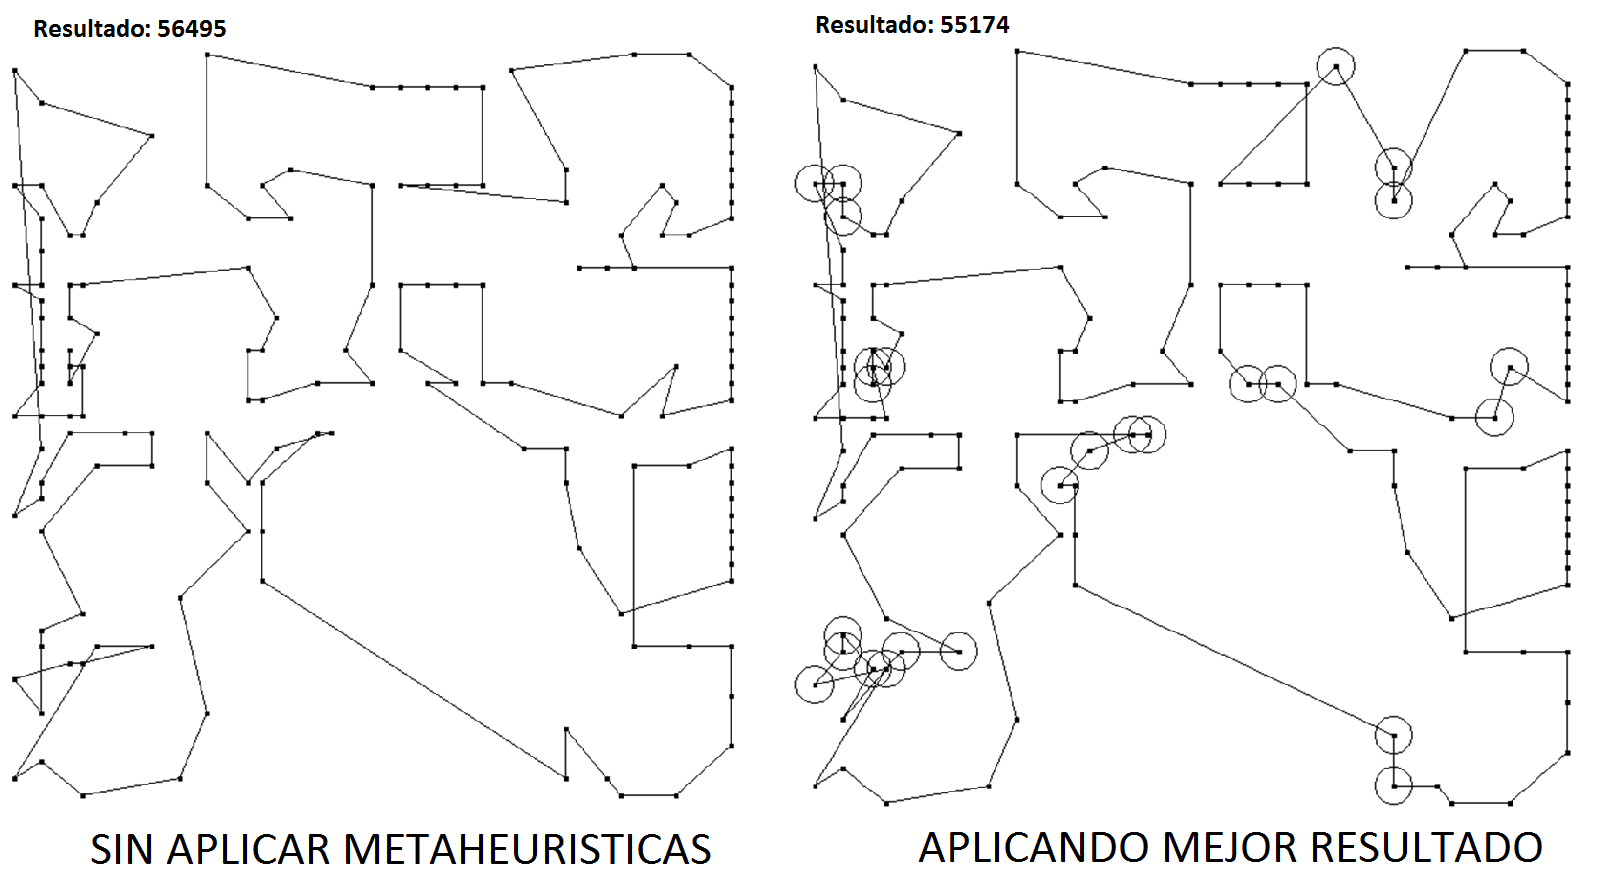
\includegraphics[width=1\textwidth]{PruebasResultados/Experimentos_Comparativas/u159.png}
        \caption{Comparativa u159.tsp}
        \label{fig:u159_comparativa.png}
\end{figure}
 \begin{figure}[hbtp]
    \centering
        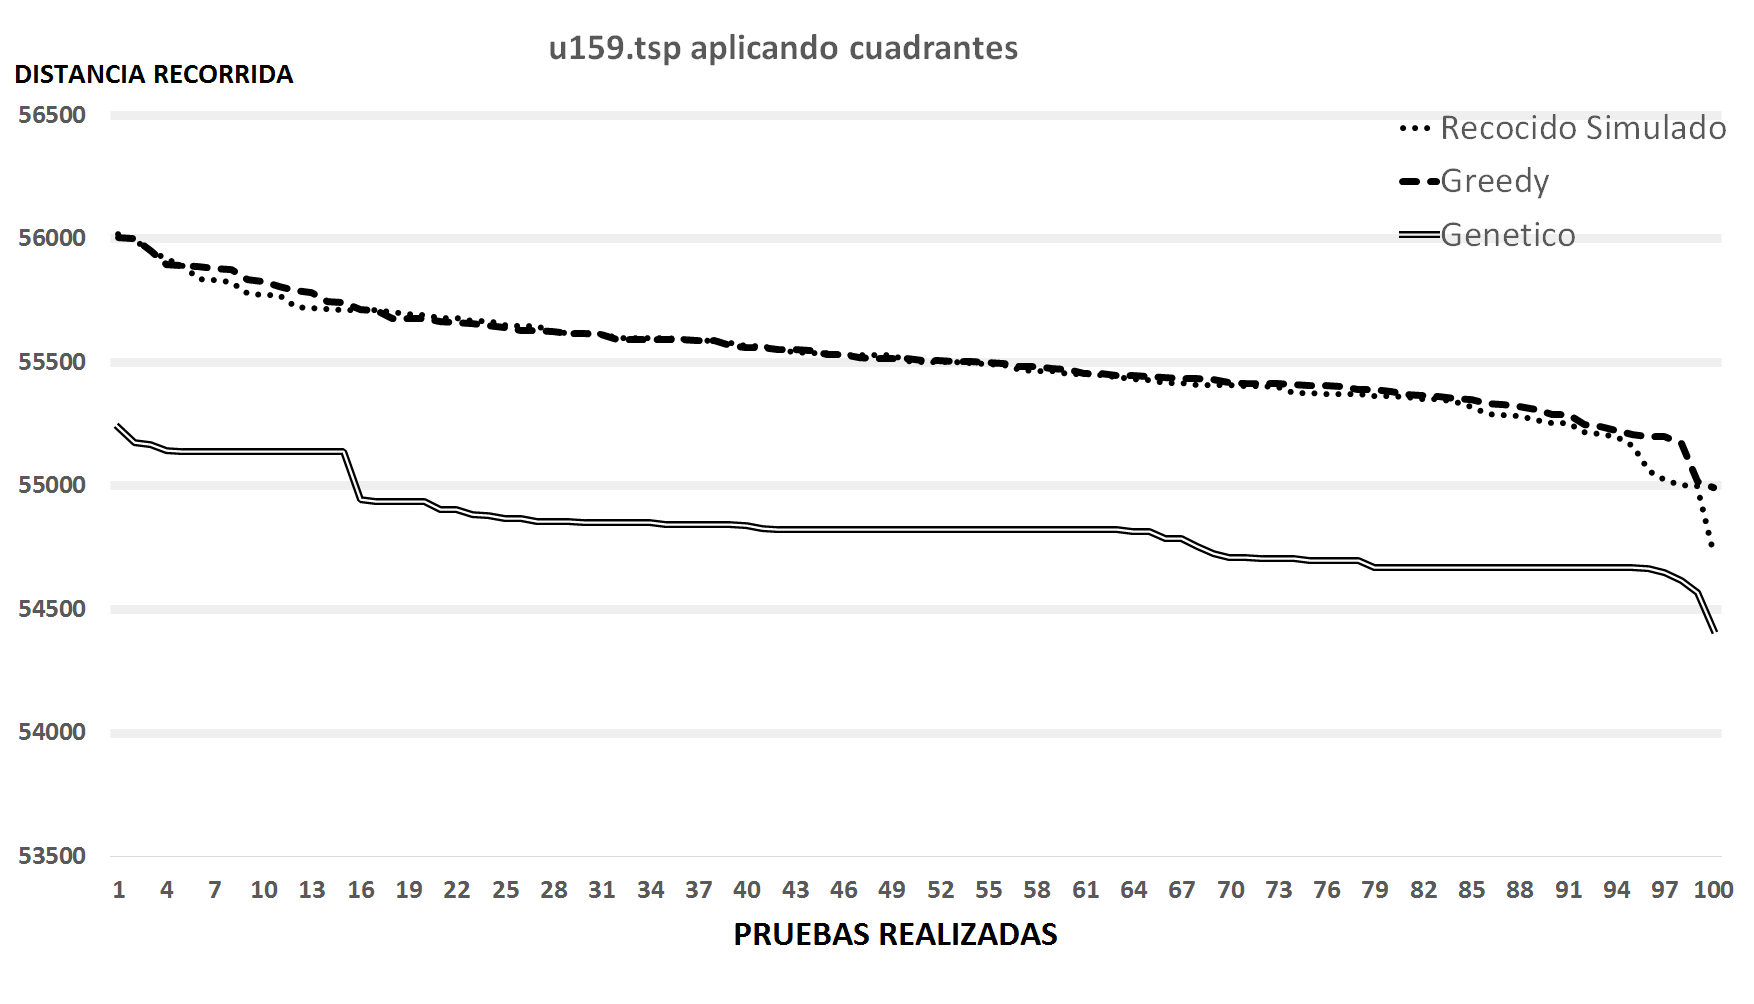
\includegraphics[width=0.9\textwidth]{PruebasResultados/Experimentos_Graficos_Con/u159.png}
        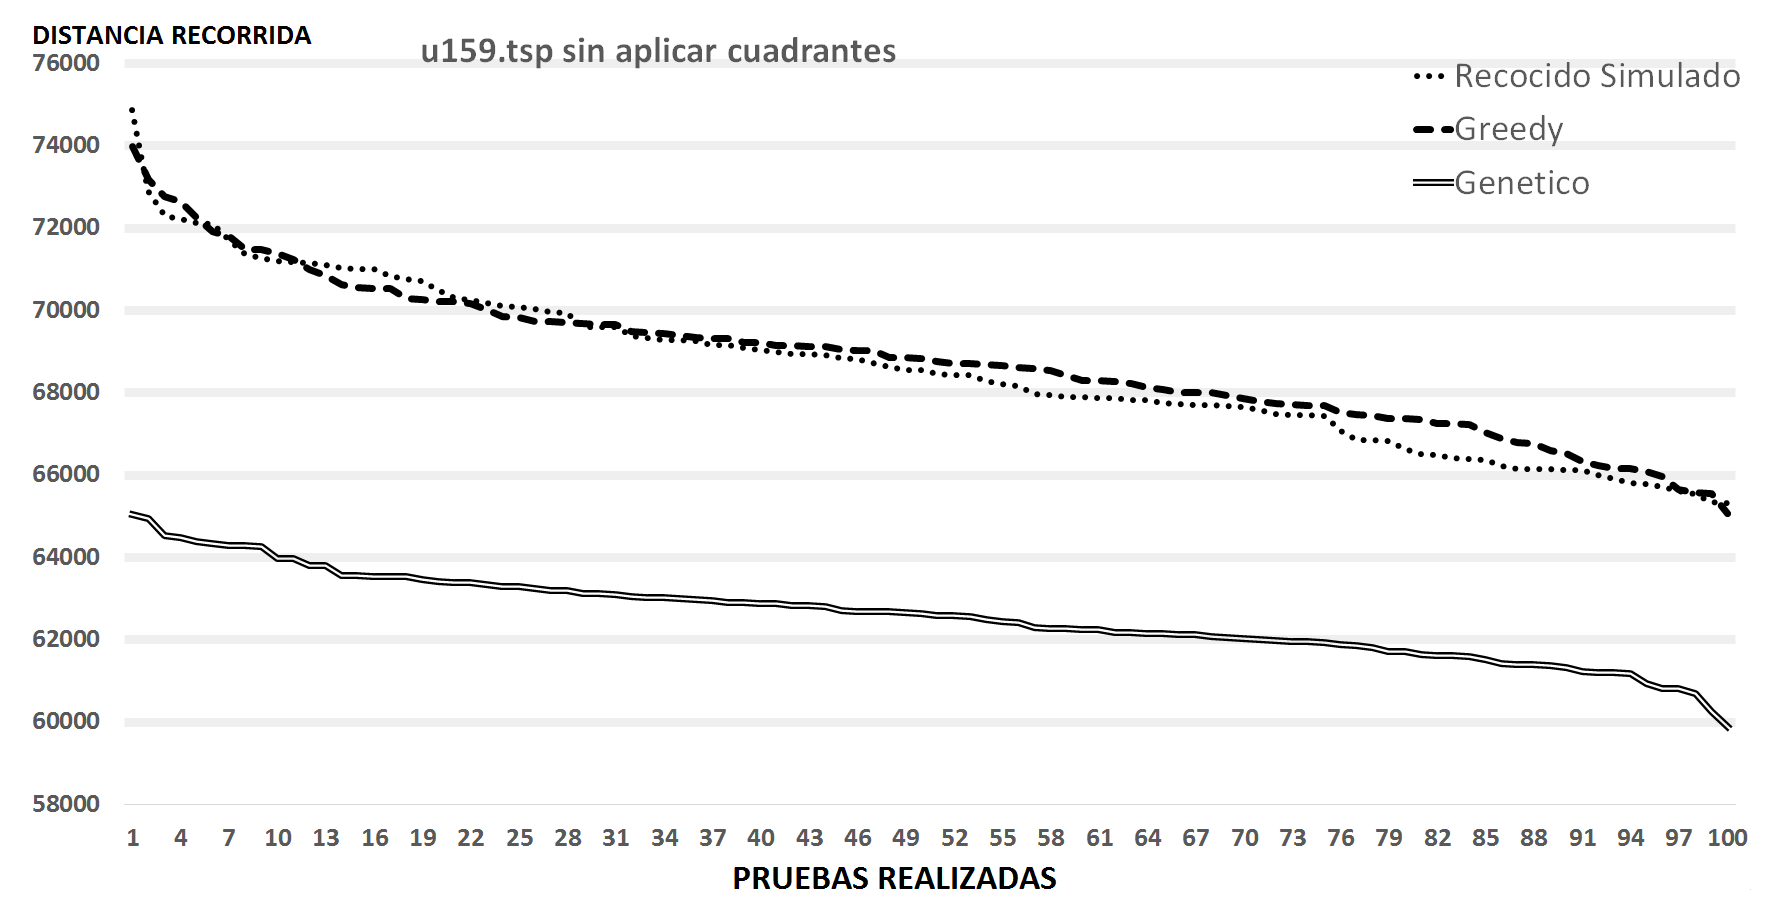
\includegraphics[width=0.9\textwidth]{PruebasResultados/Experimentos_Graficos_Sin/u159.png}
        \caption{Graficos u159.tsp con cuadrantes y sin cuadrantes}
        \label{fig:u159_grafica.png}
\end{figure}
\newpage


%MEDIANOS%%%%%%%%%%%%%%%%%%%%%%%%%%%%%%%%%%%%%%%%%%%%%%%%%%%%%%%%%%%%%%%%%%%%%%%%%%%%%%%%%%%%%%%%%%%%%%
%D493.TSP
\subsubsection{d493.TSP}
\begin{table}[hbtp]
 \centering 
	\begin{tabular}{ | l   l | r | r | r |   }
        \hline\multicolumn{5}{|c|}{ \rowcolor[gray]{0.8} d493.tsp} \\\hline
        \multicolumn{2}{|l|}{Resultado Original : 45731} & Promedio & Mejor & Peor \\ \hline
                        & Recocido  & 44582.69 & 44124 & 45012  \\ 
         Con cuadrantes & Greedy    & 44604.21 & 44054 & 45275  \\ 
                        & Genetico  & 43987.43 & 43373 & 44918  \\ \hline
                        & Recocido  & 96827.13 & 91468 & 102751   \\ 
         Sin cuadrantes & Greedy    & 96002.89 & 89956 & 100955   \\ 
                        & Genetico  & 121326.2 & 115991 & 124989    \\ \hline
    \end{tabular}
    \caption{Experimento con la prueba d493.tsp}
    \label{table:EXP_d493.tsp}
\end{table}
\begin{figure}[hbtp]
    \centering
        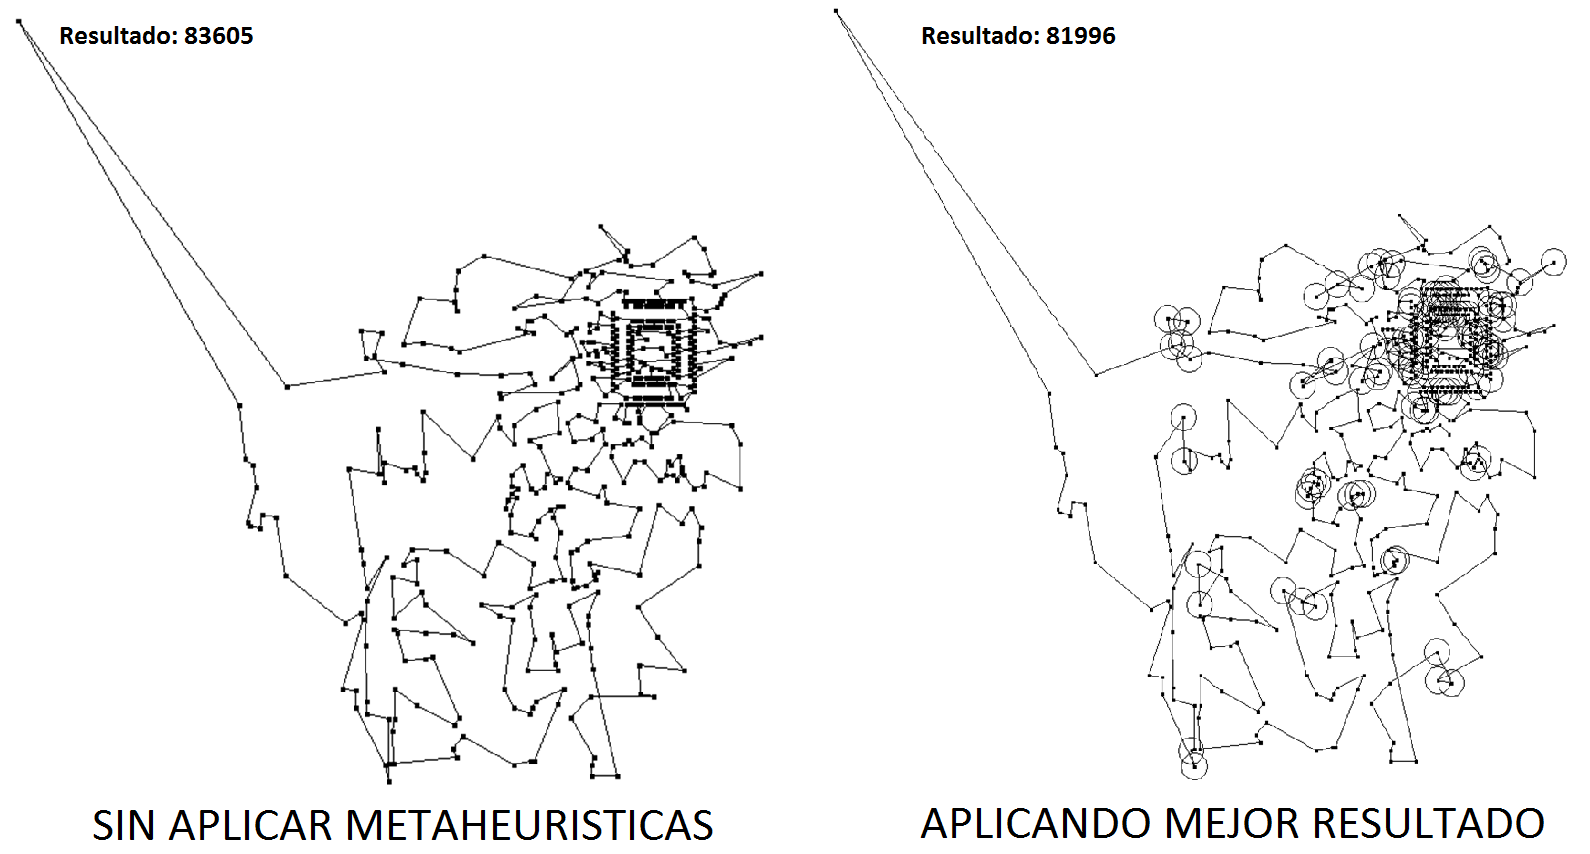
\includegraphics[width=1\textwidth]{PruebasResultados/Experimentos_Comparativas/d493.png}
        \caption{Comparativa d493.tsp}
        \label{fig:d493_comparativa.png}
\end{figure}
 \begin{figure}[hbtp]
    \centering
        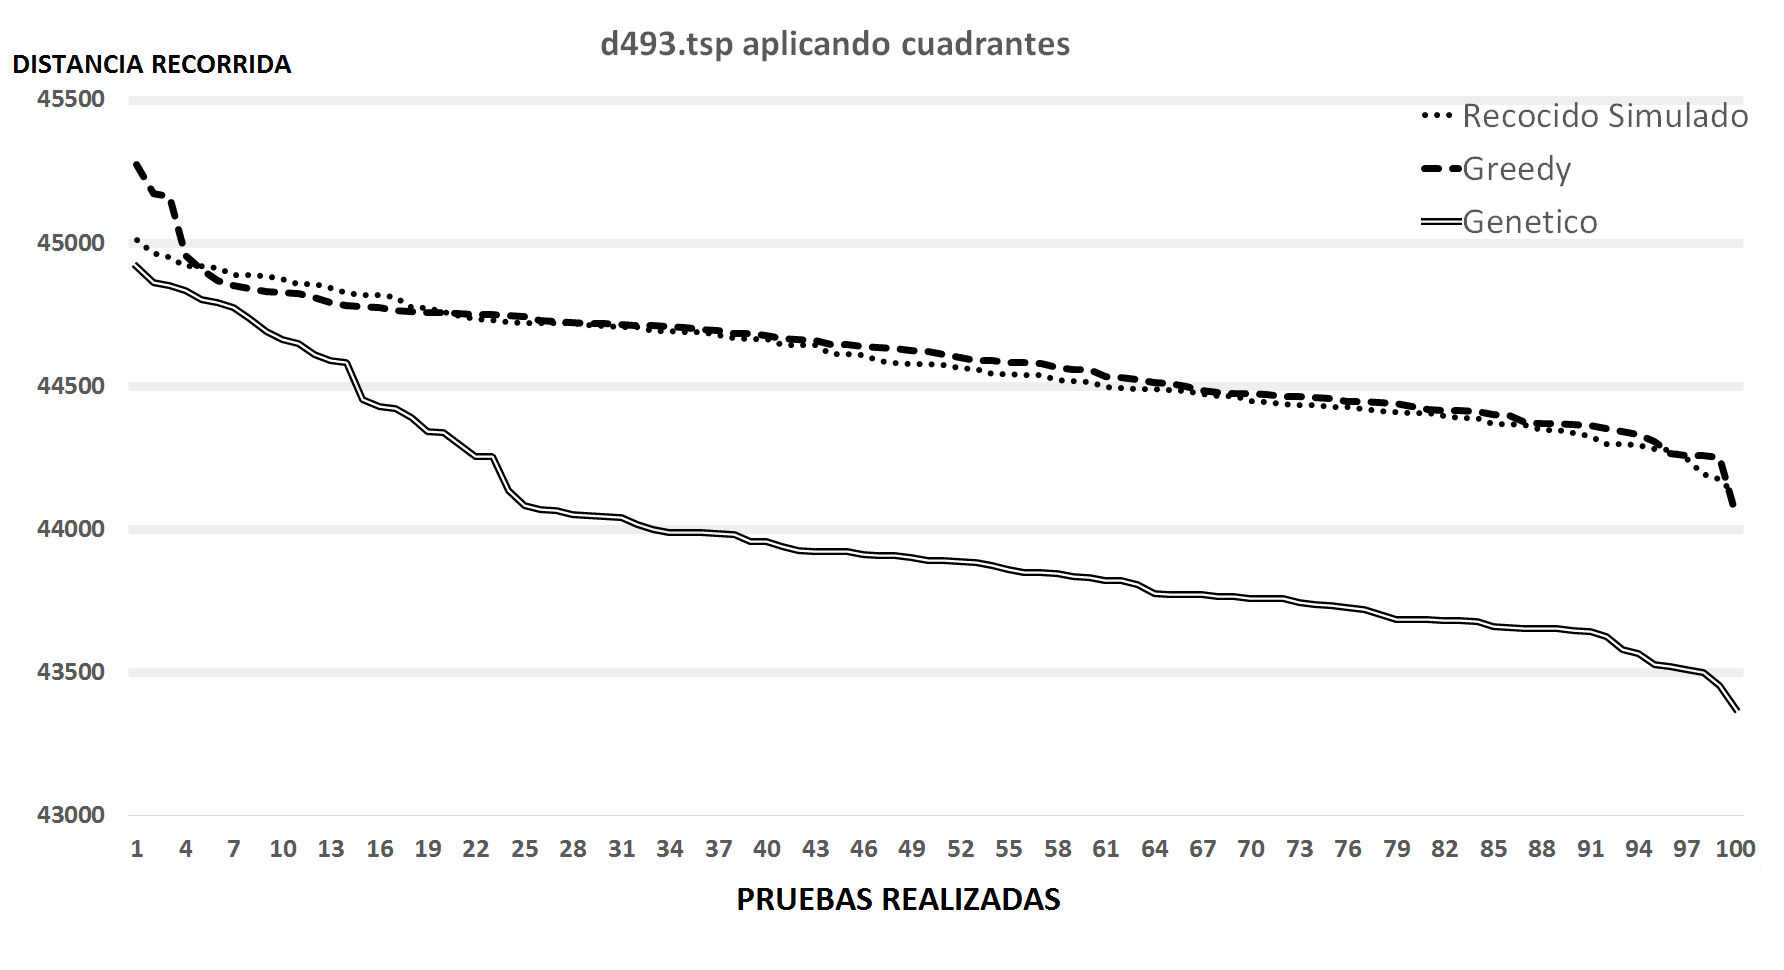
\includegraphics[width=0.9\textwidth]{PruebasResultados/Experimentos_Graficos_Con/d493.png}
        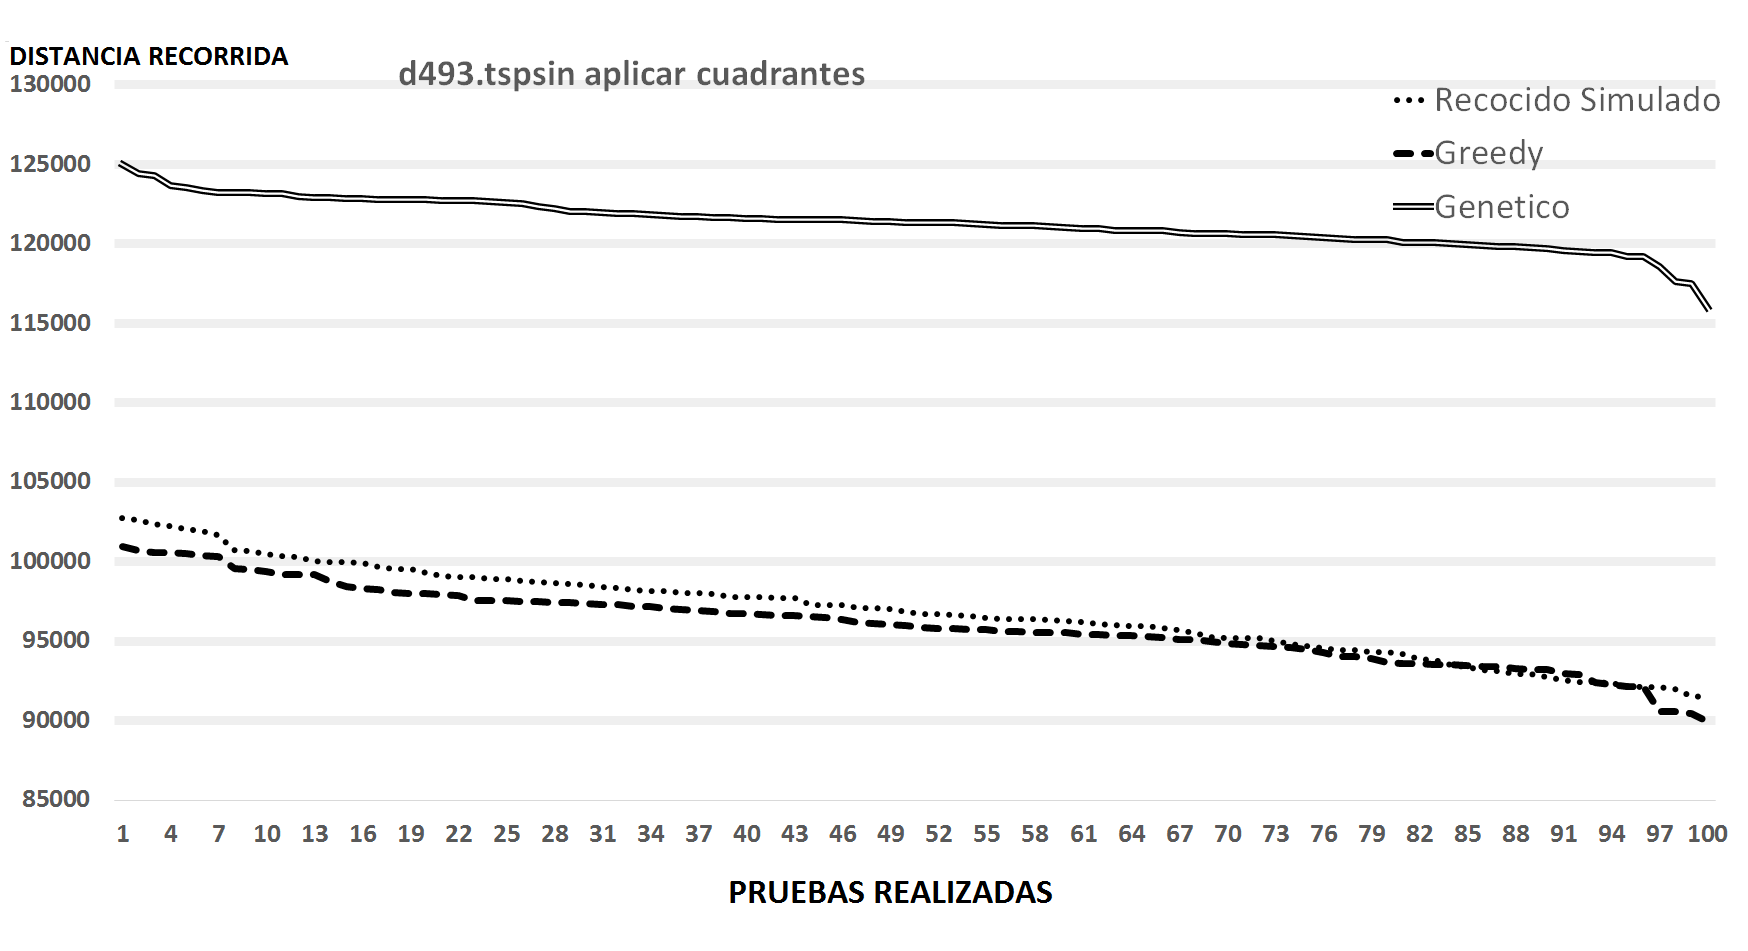
\includegraphics[width=0.9\textwidth]{PruebasResultados/Experimentos_Graficos_Sin/d493.png}
        \caption{Graficos d493.tsp con cuadrantes y sin cuadrantes}
        \label{fig:d493_grafica.png}
\end{figure}
\newpage

%fl417.TSP
\subsubsection{fl417.TSP}
\begin{table}[hbtp]
 \centering 
	\begin{tabular}{ | l   l | r | r | r |   }
       \hline\multicolumn{5}{|c|}{ \rowcolor[gray]{0.8} fl417.tsp} \\\hline
        \multicolumn{2}{|l|}{Resultado Original : 17419} & Promedio & Mejor & Peor \\ \hline
                        & Recocido  & 16835.95 & 16672 & 17070  \\ 
         Con cuadrantes & Greedy    & 16824.81 & 16610 & 17028  \\ 
                        & Genetico  & 16599.01 & 16450 & 16709  \\ \hline
                        & Recocido  & 48845.13 & 46858 & 50870   \\ 
         Sin cuadrantes & Greedy    & 48689.67 & 46460 & 50570   \\ 
                        & Genetico  & 52319.03 & 50896 & 53761    \\ \hline
    \end{tabular}
    \caption{Experimento con la prueba fl417.tsp}
    \label{table:EXP_fl417.tsp}
\end{table}
\begin{figure}[hbtp]
    \centering
        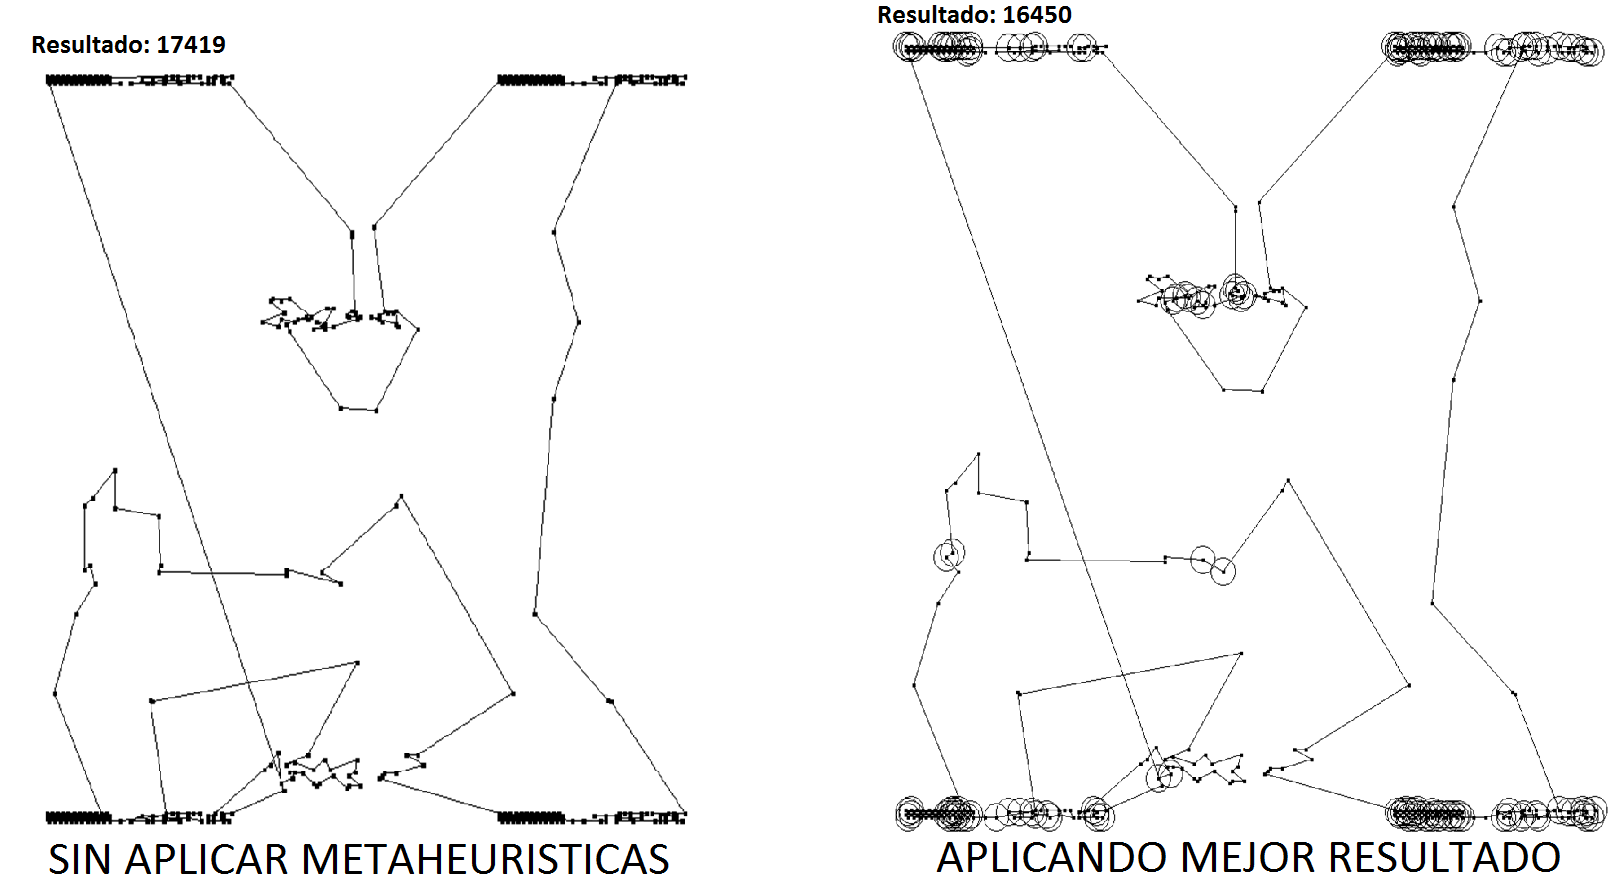
\includegraphics[width=1\textwidth]{PruebasResultados/Experimentos_Comparativas/fl417.png}
        \caption{Comparativa fl417.tsp}
        \label{fig:fl417_comparativa.png}
\end{figure}
 \begin{figure}[hbtp]
    \centering
        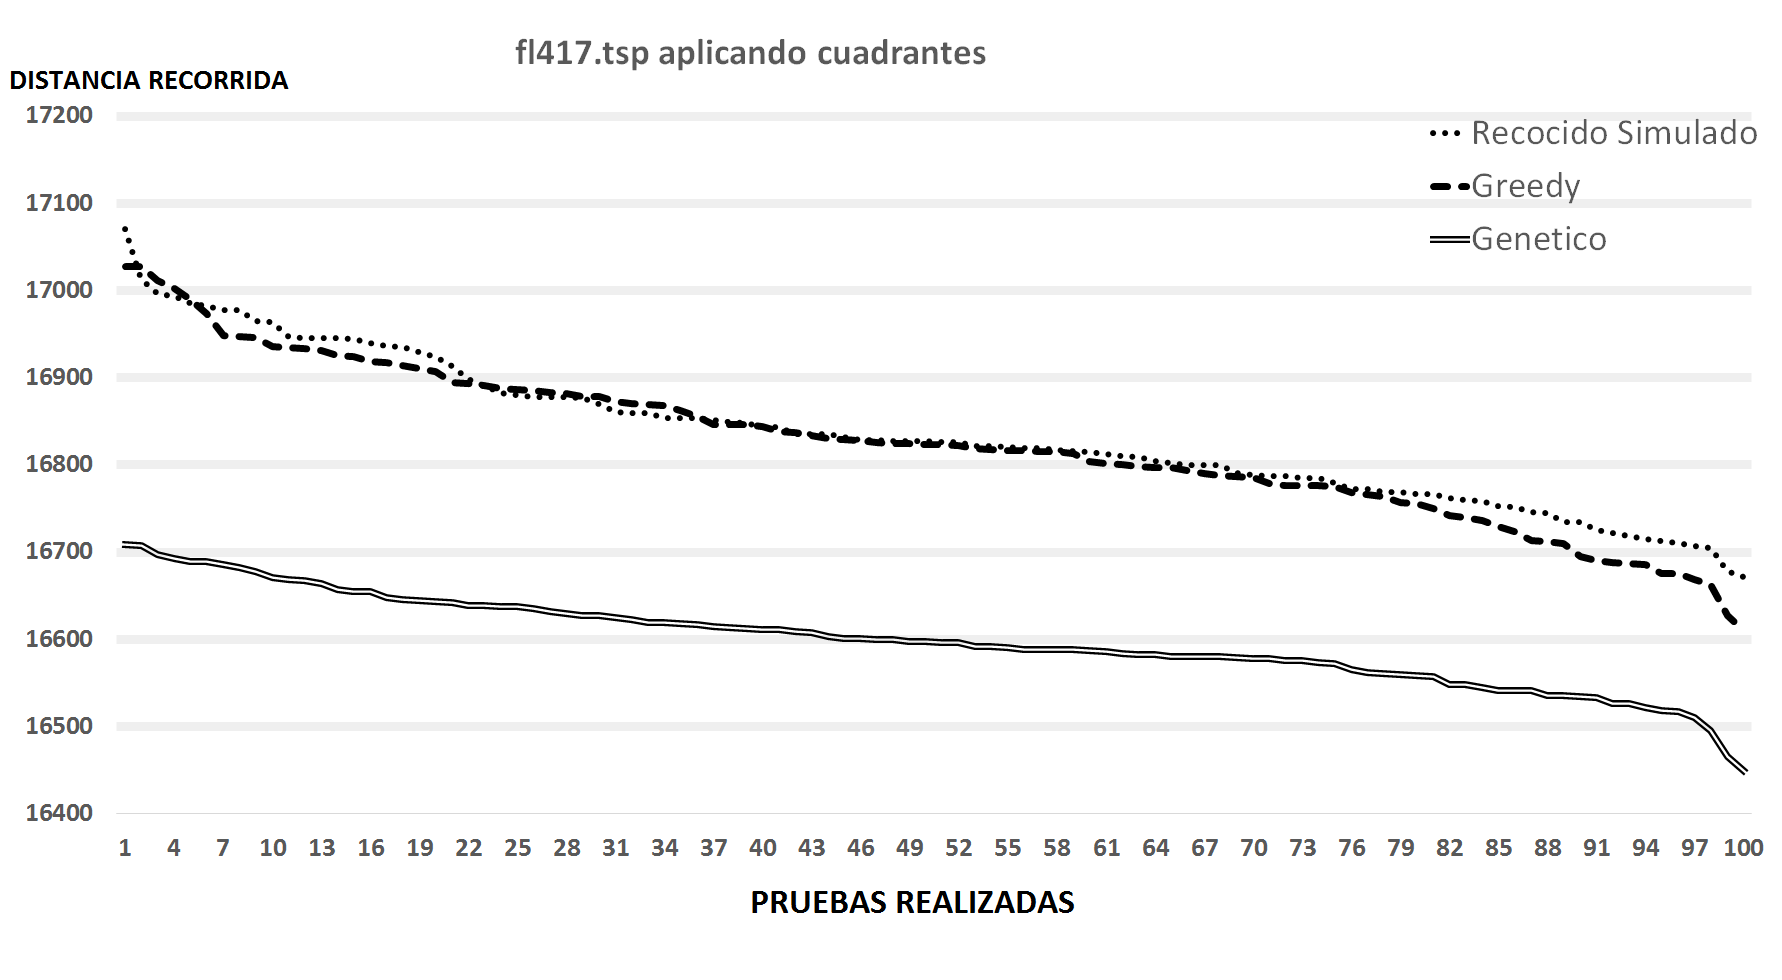
\includegraphics[width=0.9\textwidth]{PruebasResultados/Experimentos_Graficos_Con/fl417.png}
        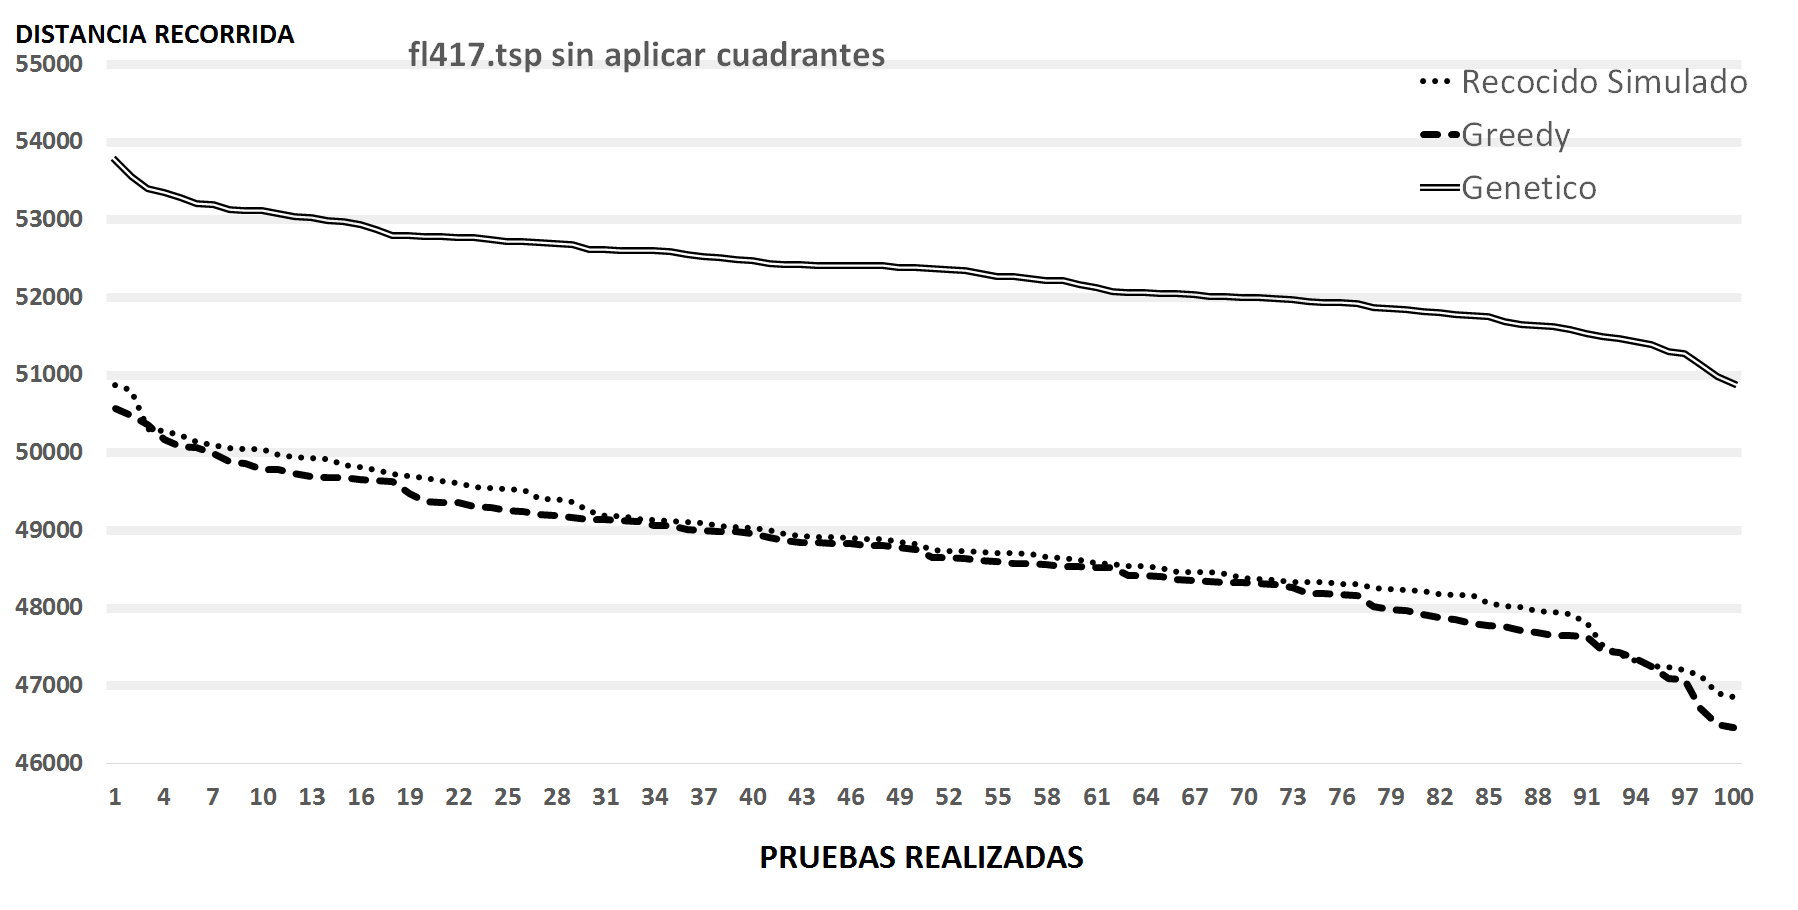
\includegraphics[width=0.9\textwidth]{PruebasResultados/Experimentos_Graficos_Sin/fl417.png}
        \caption{Graficos fl417.tsp con cuadrantes y sin cuadrantes}
        \label{fig:fl417_grafica.png}
\end{figure}
\newpage

%P654.TSP
\subsubsection{p654.TSP}
\begin{table}[hbtp]
 \centering 
	\begin{tabular}{ | l   l | r | r | r |   }
        \hline\multicolumn{5}{|c|}{ \rowcolor[gray]{0.8}p654.tsp} \\\hline
         \multicolumn{2}{|l|}{Resultado Original : 47464} & Promedio & Mejor & Peor \\ \hline
                        & Recocido  & 46190.13 & 45753 & 46767  \\ 
         Con cuadrantes & Greedy    & 46146.53 & 45588 & 46541  \\ 
                        & Genetico  & 45916.31 & 45645 & 46292  \\ \hline
                        & Recocido  & 121597.61 & 118683 & 127226   \\ 
         Sin cuadrantes & Greedy    & 121537.77 & 118676 & 126211   \\ 
                        & Genetico  & 132643.30 & 131454 & 135144    \\ \hline
    \end{tabular}
    \caption{Experimento con la prueba p654.tsp}
    \label{table:EXP_p654.tsp}
\end{table}
\begin{figure}[hbtp]
    \centering
        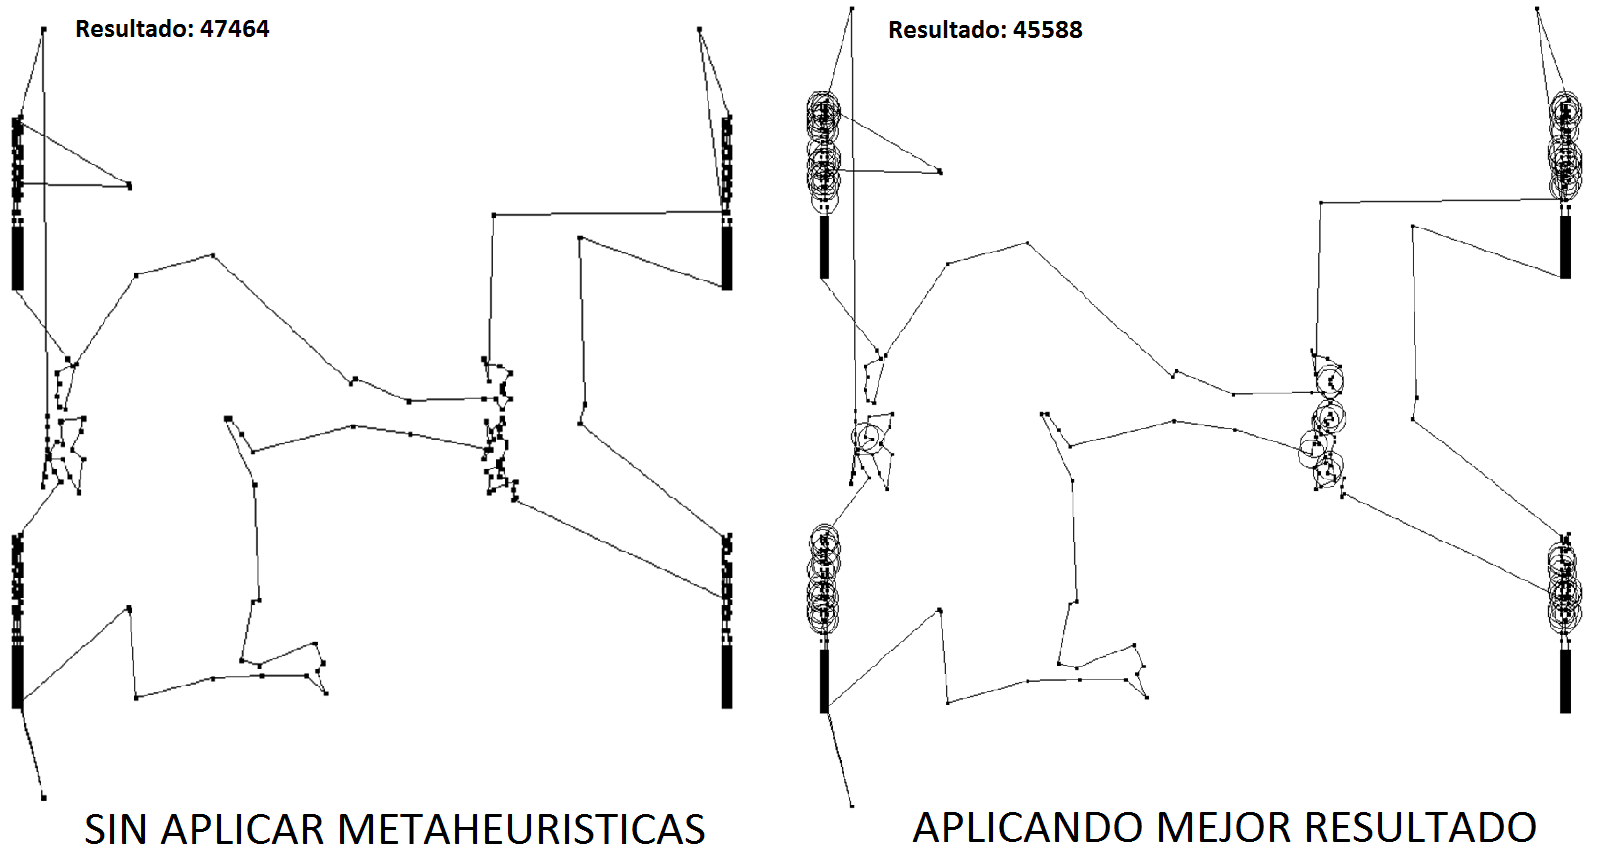
\includegraphics[width=1\textwidth]{PruebasResultados/Experimentos_Comparativas/p654.png}
        \caption{Comparativa p654.tsp}
        \label{fig:p654_comparativa.png}
\end{figure}
 \begin{figure}[hbtp]
    \centering
        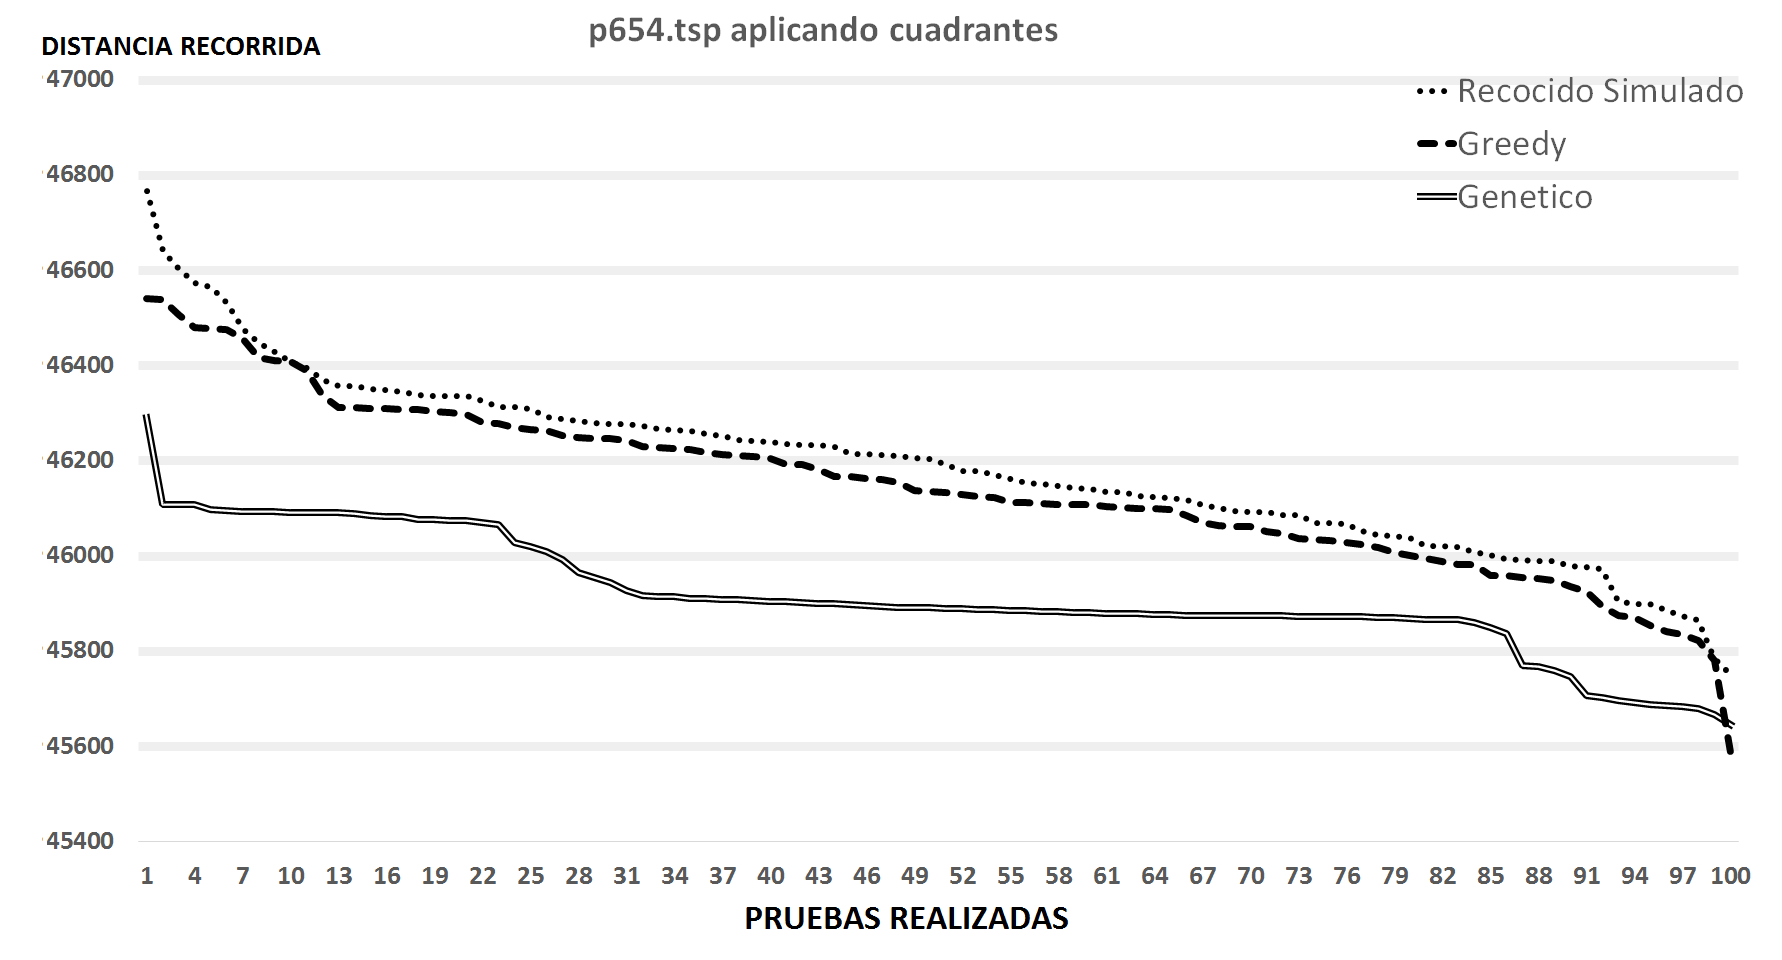
\includegraphics[width=0.9\textwidth]{PruebasResultados/Experimentos_Graficos_Con/p654.png}
        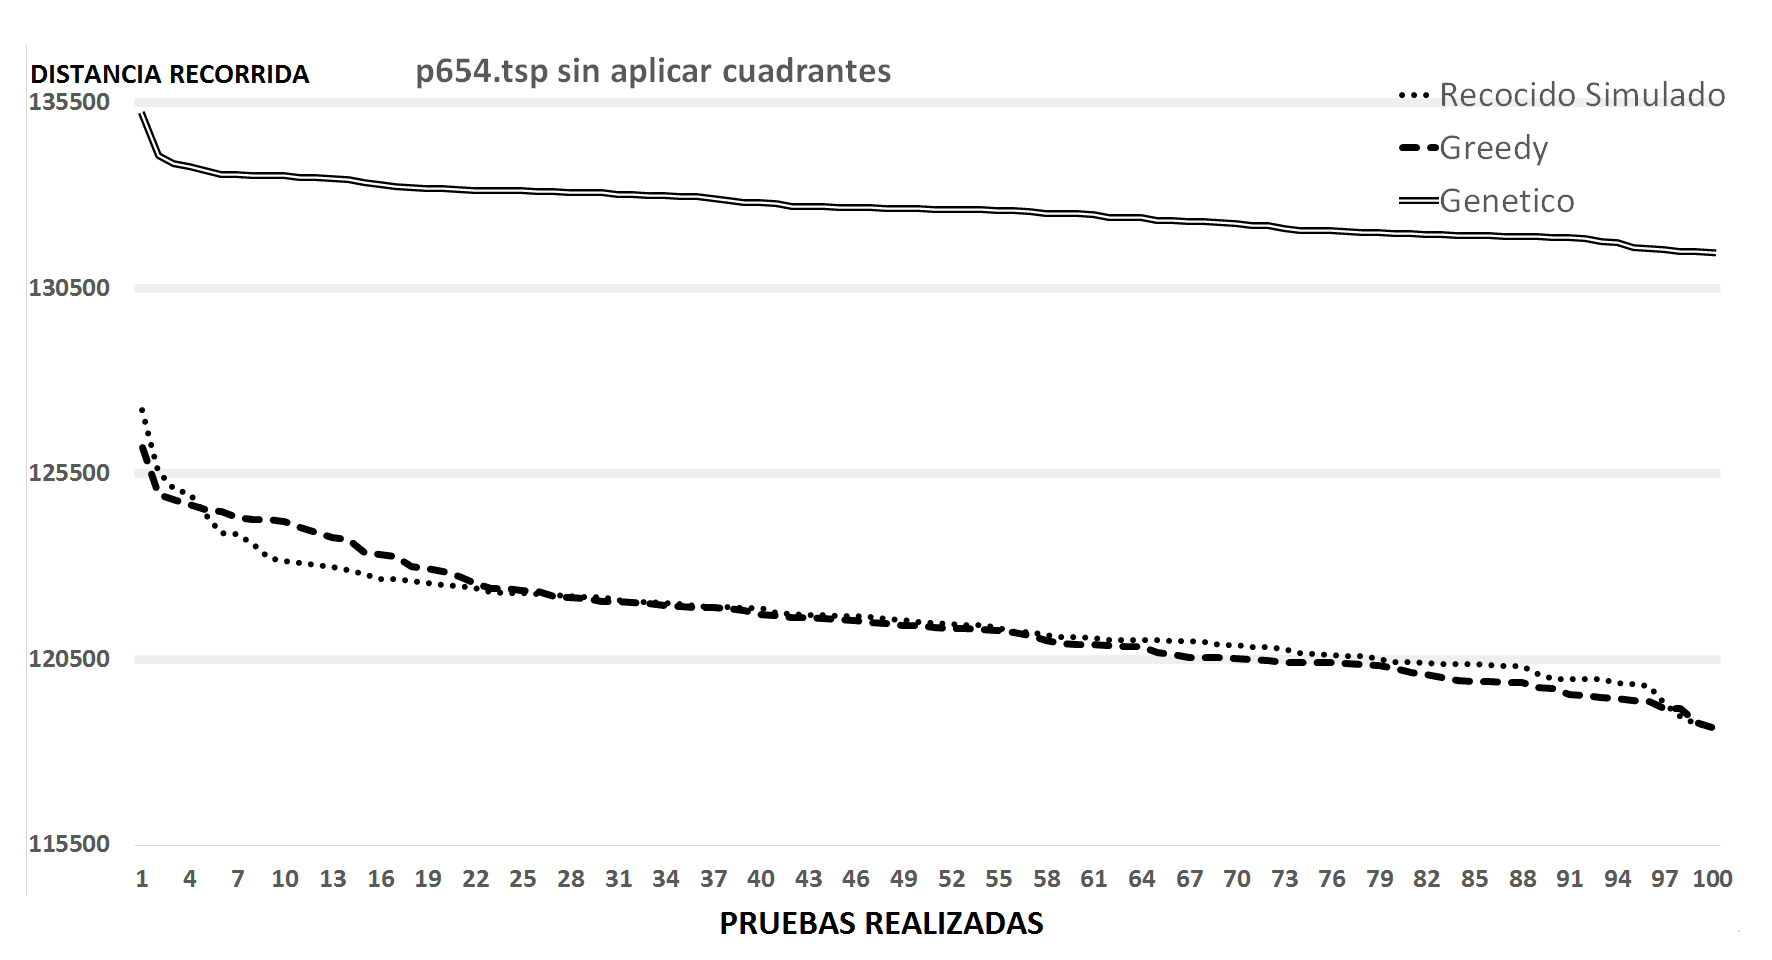
\includegraphics[width=0.9\textwidth]{PruebasResultados/Experimentos_Graficos_Sin/p654.png}
        \caption{Graficos p654.tsp con cuadrantes y sin cuadrantes}
        \label{fig:p654_grafica.png}
\end{figure}
\newpage

%rd400.TSP
\subsubsection{rd400.TSP}
\begin{table}[hbtp]
 \centering 
	\begin{tabular}{ | l   l | r | r | r |   }
        \hline\multicolumn{5}{|c|}{ \rowcolor[gray]{0.8}rd400.tsp } \\\hline
         \multicolumn{2}{|l|}{Resultado Original : 19094} & Promedio & Mejor & Peor \\ \hline
                        & Recocido  & 18773.66 & 18562 & 18922  \\ 
         Con cuadrantes & Greedy    & 18766.69 & 18559 & 18919  \\ 
                        & Genetico  & 18633.28 & 18510 & 18790  \\ \hline
                        & Recocido  & 109863.35 & 101860 & 118554   \\ 
         Sin cuadrantes & Greedy    & 109948.16 & 102698 & 117363   \\ 
                        & Genetico  & 178000.38 & 174218 & 181970   \\ \hline
    \end{tabular}
    \caption{Experimento con la prueba rd400.tsp}
    \label{table:EXP_rd400.tsp}
\end{table}
\begin{figure}[hbtp]
    \centering
        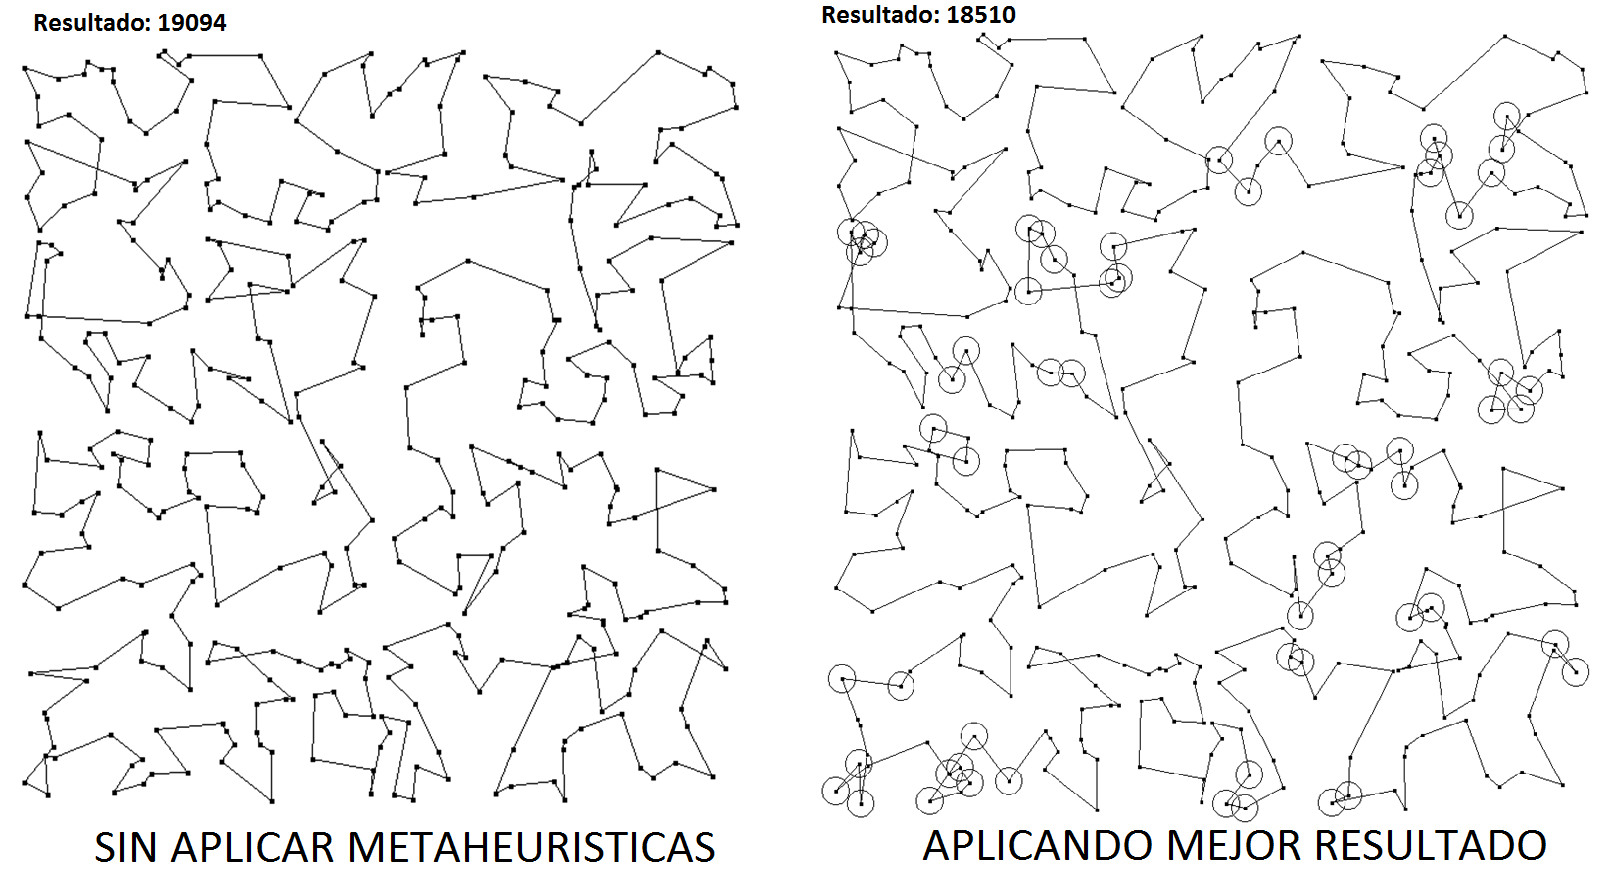
\includegraphics[width=1\textwidth]{PruebasResultados/Experimentos_Comparativas/rd400.png}
        \caption{Comparativa rd400.tsp}
        \label{fig:rd400_comparativa.png}
\end{figure}
 \begin{figure}[hbtp]
    \centering
        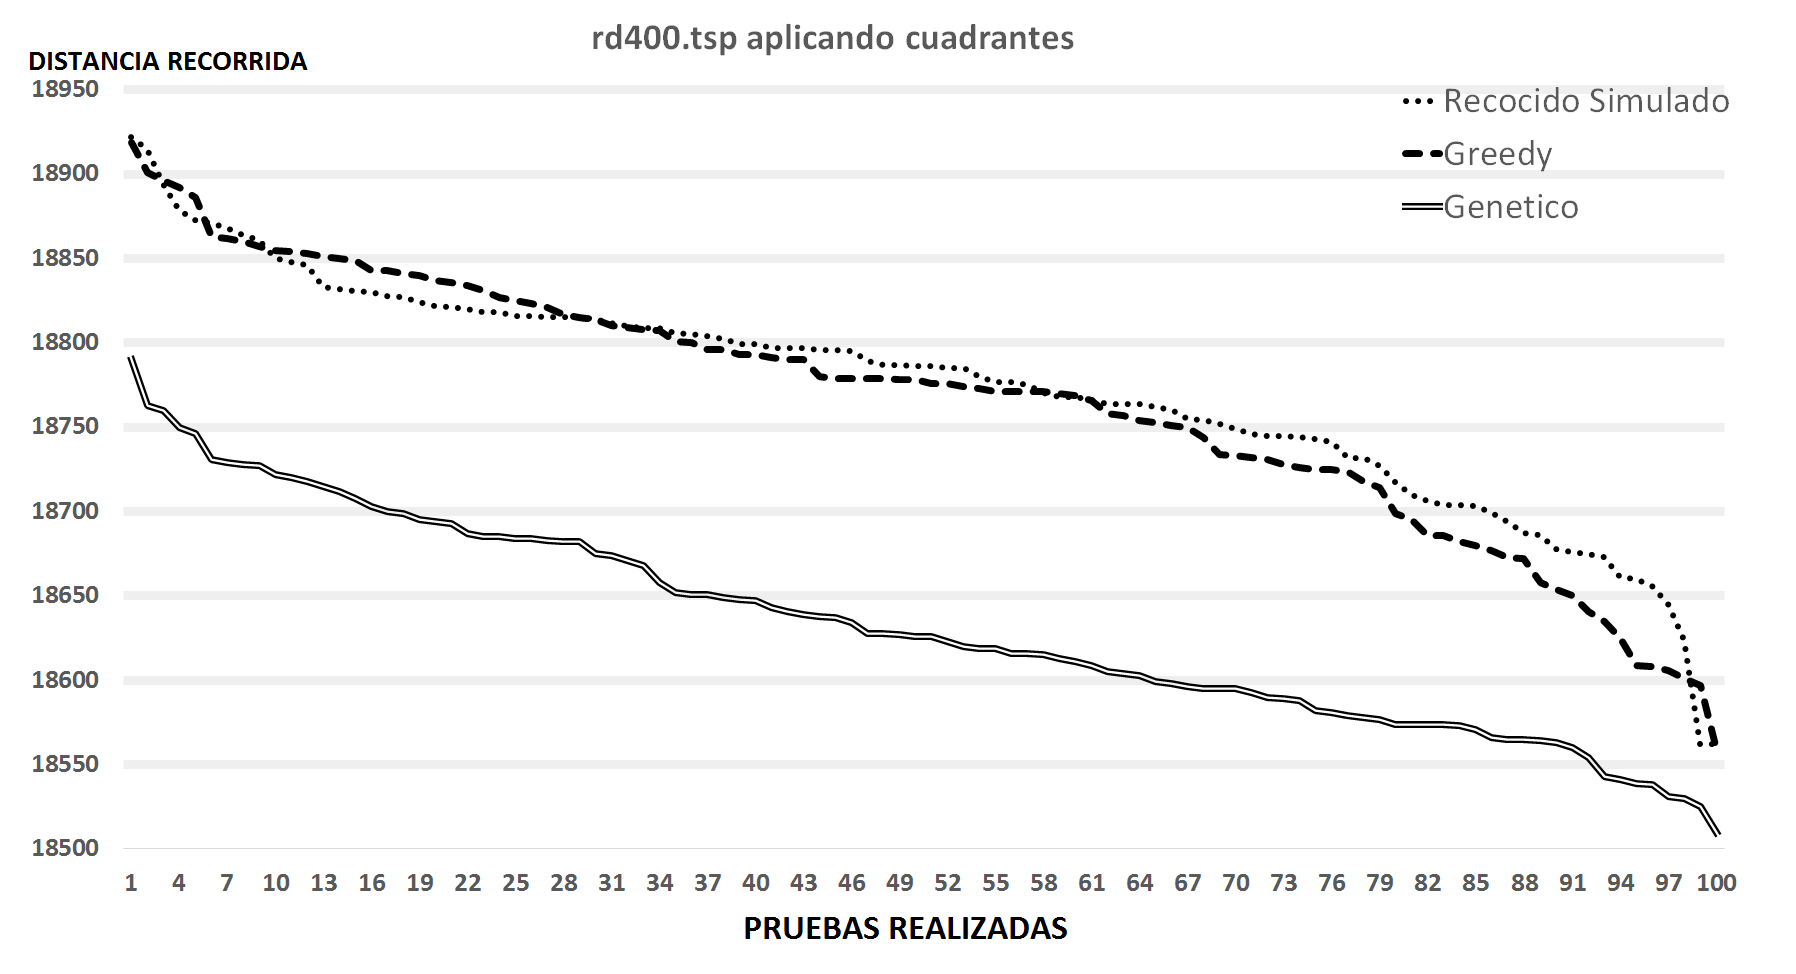
\includegraphics[width=0.9\textwidth]{PruebasResultados/Experimentos_Graficos_Con/rd400.png}
        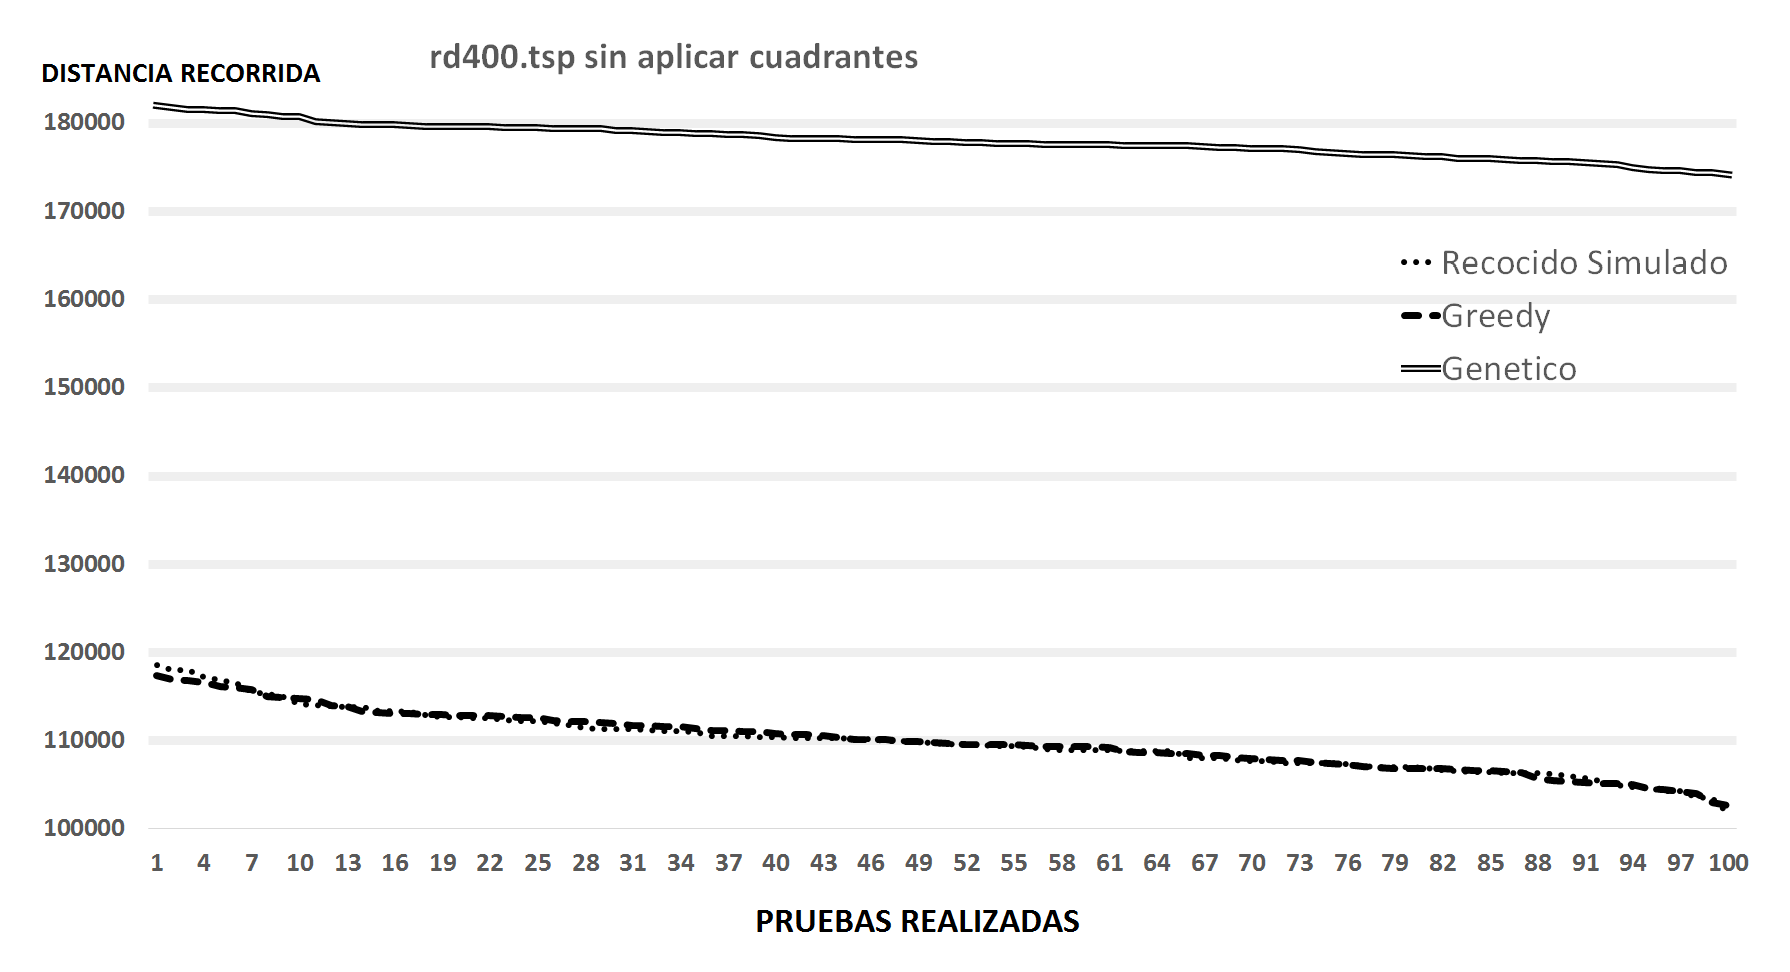
\includegraphics[width=0.9\textwidth]{PruebasResultados/Experimentos_Graficos_Sin/rd400.png}
        \caption{Graficos rd400.tsp con cuadrantes y sin cuadrantes}
        \label{fig:rd400_grafica.png}
\end{figure}
\newpage

%u724.TSP
\subsubsection{u724.TSP}
\begin{table}[hbtp]
 \centering 
	\begin{tabular}{ | l   l | r | r | r |   }
         \hline\multicolumn{5}{|c|}{ \rowcolor[gray]{0.8}u724.tsp } \\\hline
         \multicolumn{2}{|l|}{Resultado Original : 57641} & Promedio & Mejor & Peor \\ \hline
                        & Recocido  & 55976.89 & 55514 & 56479  \\ 
         Con cuadrantes & Greedy    & 56010.58 & 55474 & 56725  \\ 
                        & Genetico  & 55004.45 & 54685 & 55283  \\ \hline
                        & Recocido  & 140950.1 & 134129 & 149630   \\ 
         Sin cuadrantes & Greedy    & 140872.24 & 132686 & 149355   \\ 
                        & Genetico  & 168973.59 & 164770 & 171946   \\ \hline
    \end{tabular}
    \caption{Experimento con la prueba u724.tsp}
    \label{table:EXP_u724.tsp}
\end{table}	
\begin{figure}[hbtp]
    \centering
        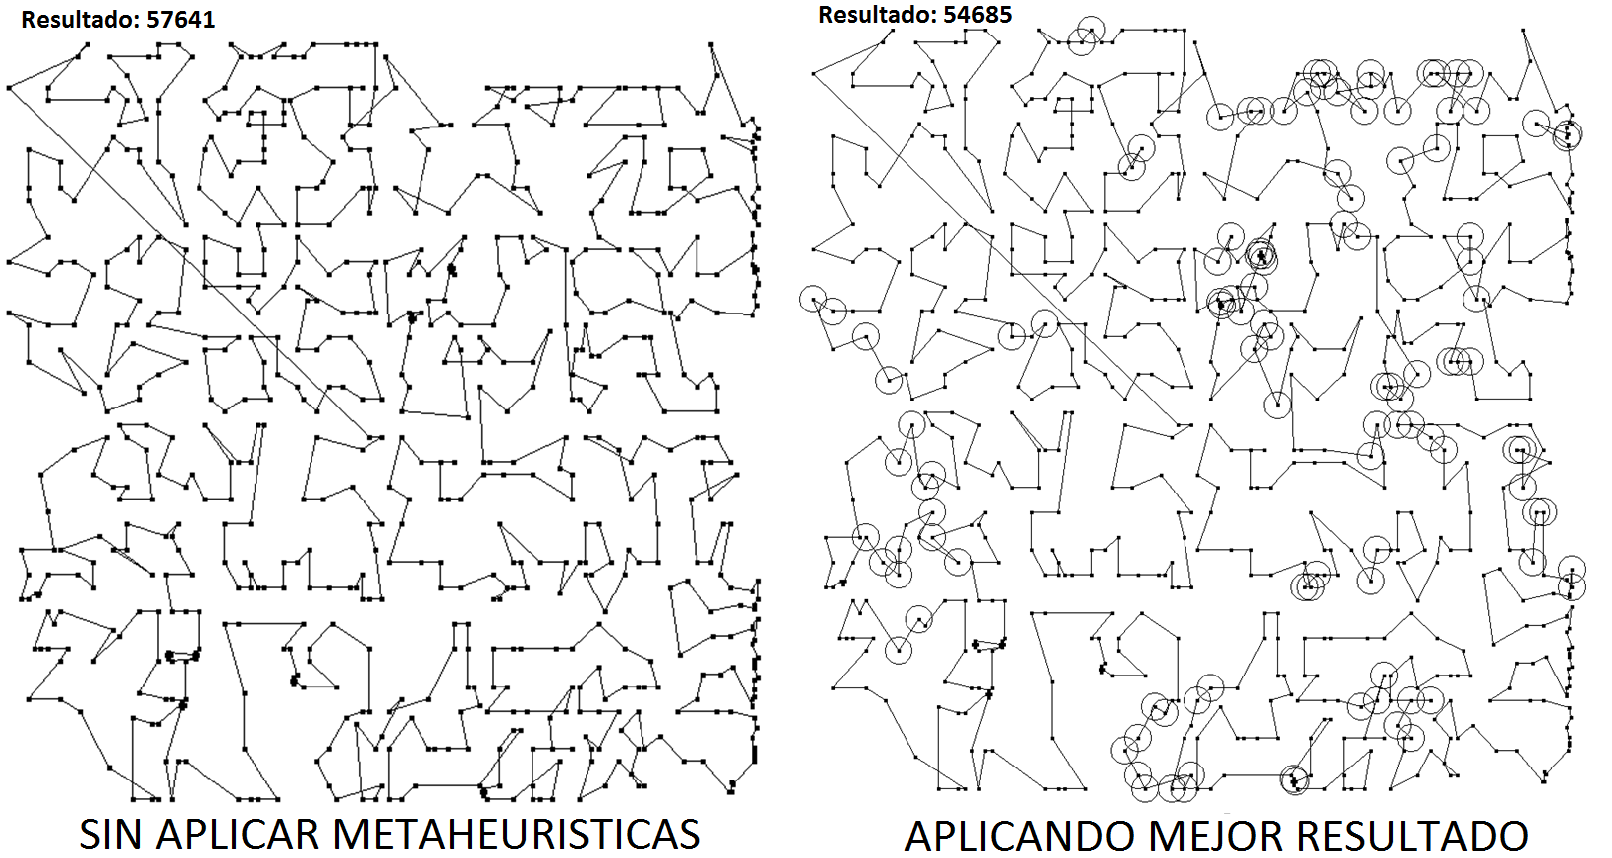
\includegraphics[width=1\textwidth]{PruebasResultados/Experimentos_Comparativas/u724.png}
        \caption{Comparativa u724.tsp}
        \label{fig:u724_comparativa.png}
\end{figure}
 \begin{figure}[hbtp]
    \centering
        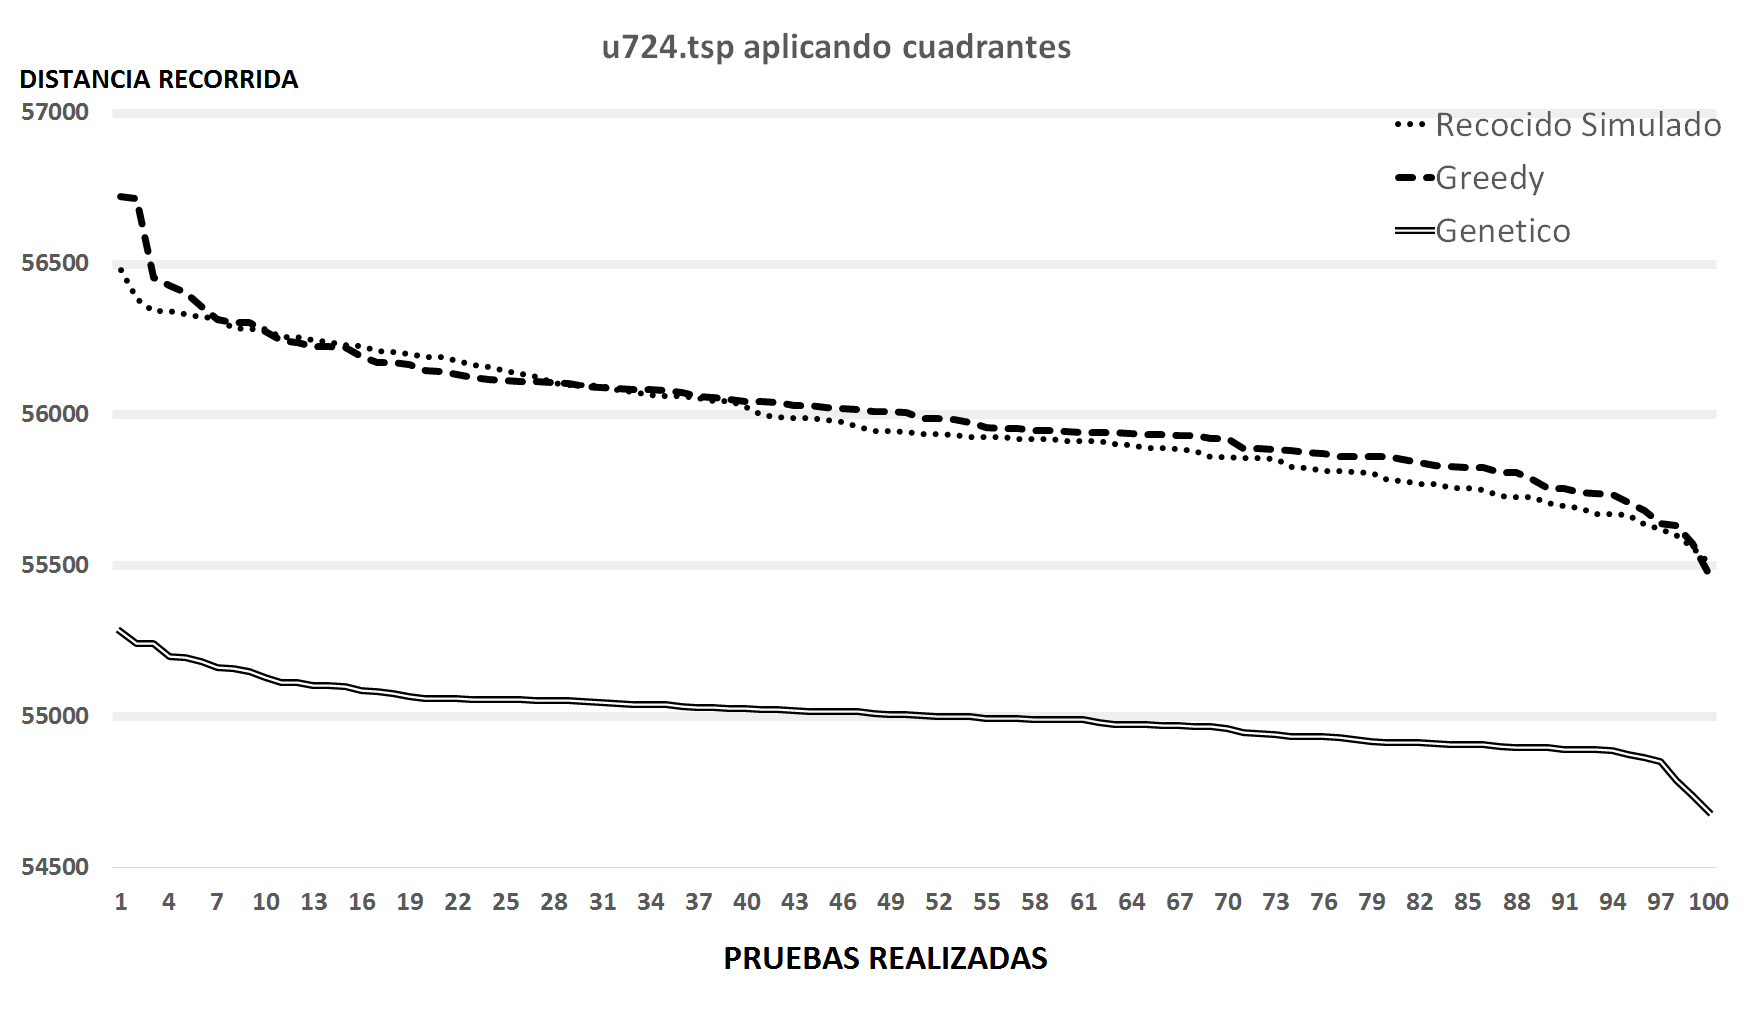
\includegraphics[width=0.9\textwidth]{PruebasResultados/Experimentos_Graficos_Con/u724.png}
        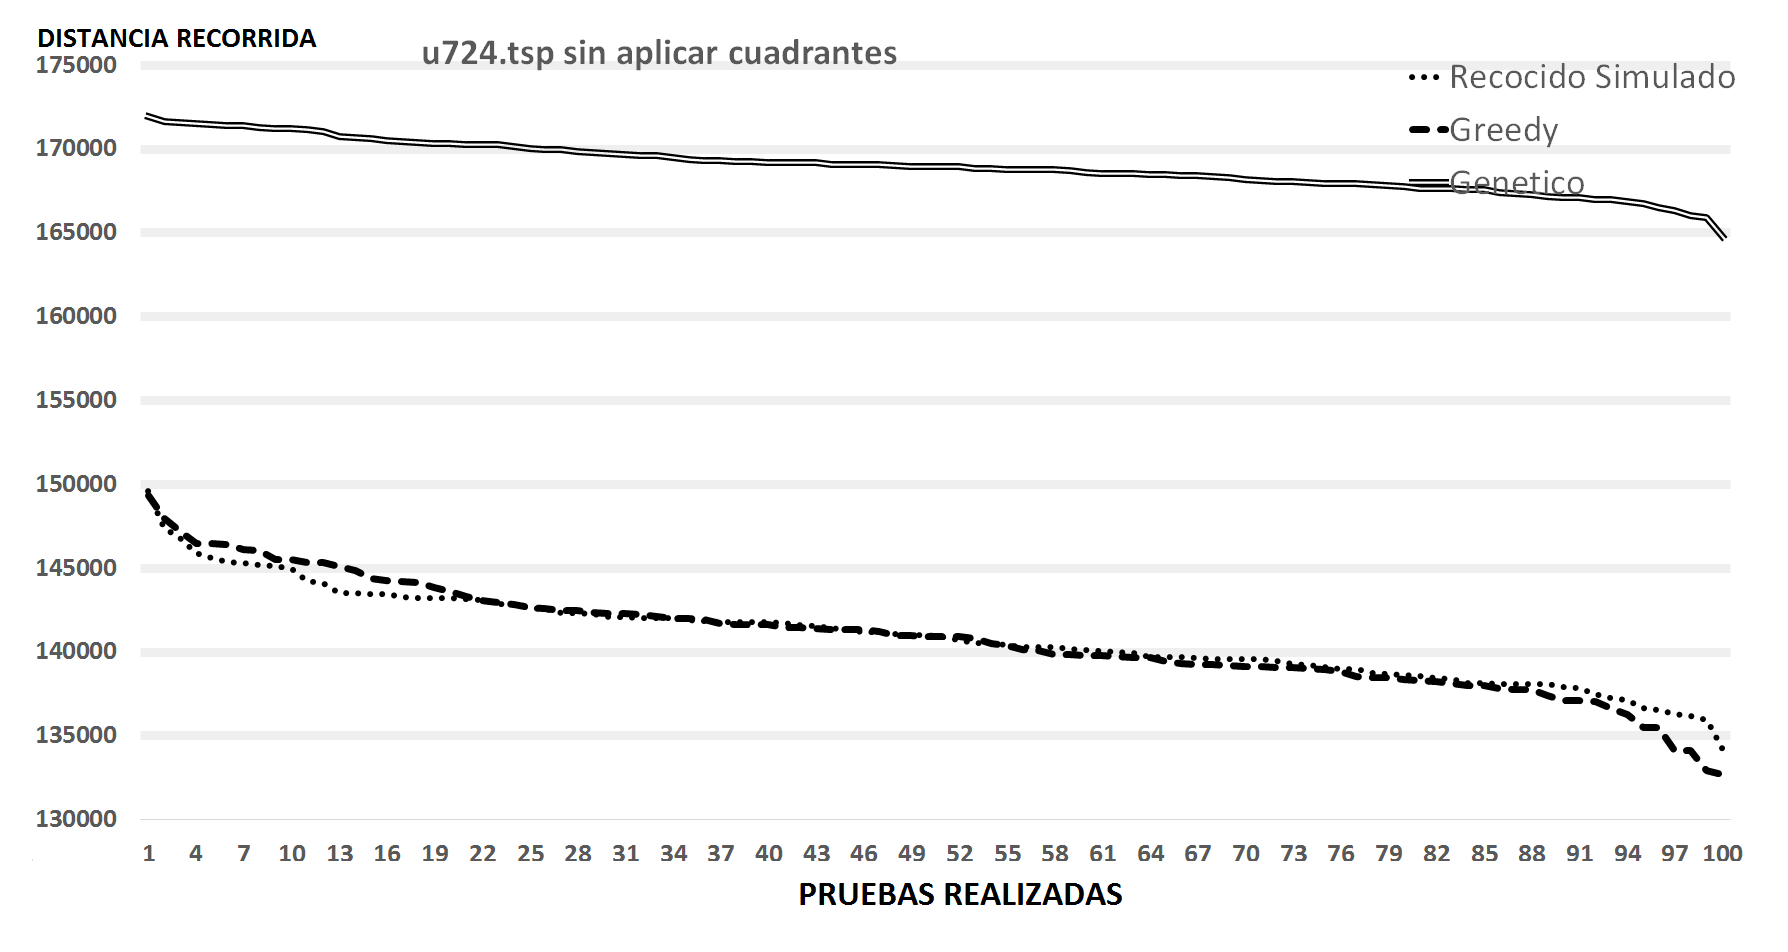
\includegraphics[width=0.9\textwidth]{PruebasResultados/Experimentos_Graficos_Sin/u724.png}
        \caption{Graficos u724.tsp con cuadrantes y sin cuadrantes}
        \label{fig:u724_grafica.png}
\end{figure}
\newpage

%GRANDES
%brd14051.TSP
\subsubsection{brd14051.TSP}
\begin{table}[hbtp]
 \centering 
	\begin{tabular}{ | l   l | r | r | r |   }
        \hline\multicolumn{5}{|c|}{ \rowcolor[gray]{0.8}brd14051.tsp  } \\\hline
        \multicolumn{2}{|l|}{Resultado Original :623324}  & Promedio & Mejor & Peor \\ \hline
                        & Recocido  & 619876.89 & 618878 & 620546  \\ 
         Con cuadrantes & Greedy    & 619899.03 & 619060 & 620743  \\ 
                        & Genetico  & 621842.3 & 621273 & 622688  \\ \hline
                        & Recocido  & 13091307.46 & 12612710 & 13458979   \\ 
         Sin cuadrantes & Greedy    & 13071094.56 & 12811921 & 13411800   \\ 
                        & Genetico  & 23478563.4 & 23433764 & 23520252   \\ \hline
    \end{tabular}
    \caption{Experimento con la prueba brd14051.tsp}
    \label{table:EXP_brd14051.tsp}
\end{table}
\begin{figure}[hbtp]
    \centering
        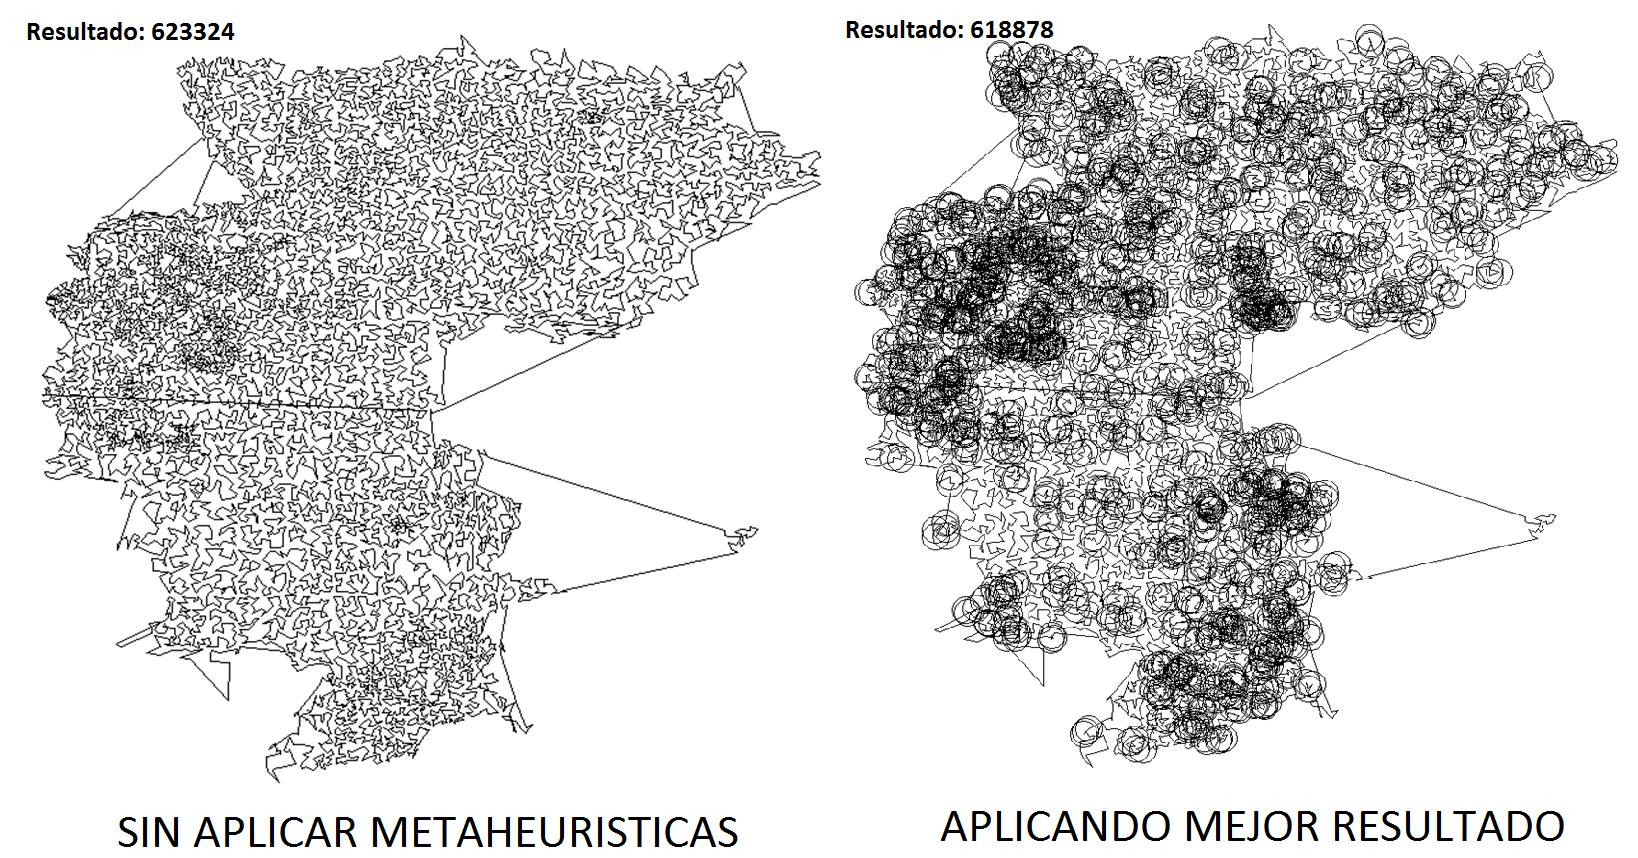
\includegraphics[width=1\textwidth]{PruebasResultados/Experimentos_Comparativas/brd14051.png}
        \caption{Comparativa brd14051.tsp}
        \label{fig:brd14051_comparativa.png}
\end{figure}
 \begin{figure}[hbtp]
    \centering
        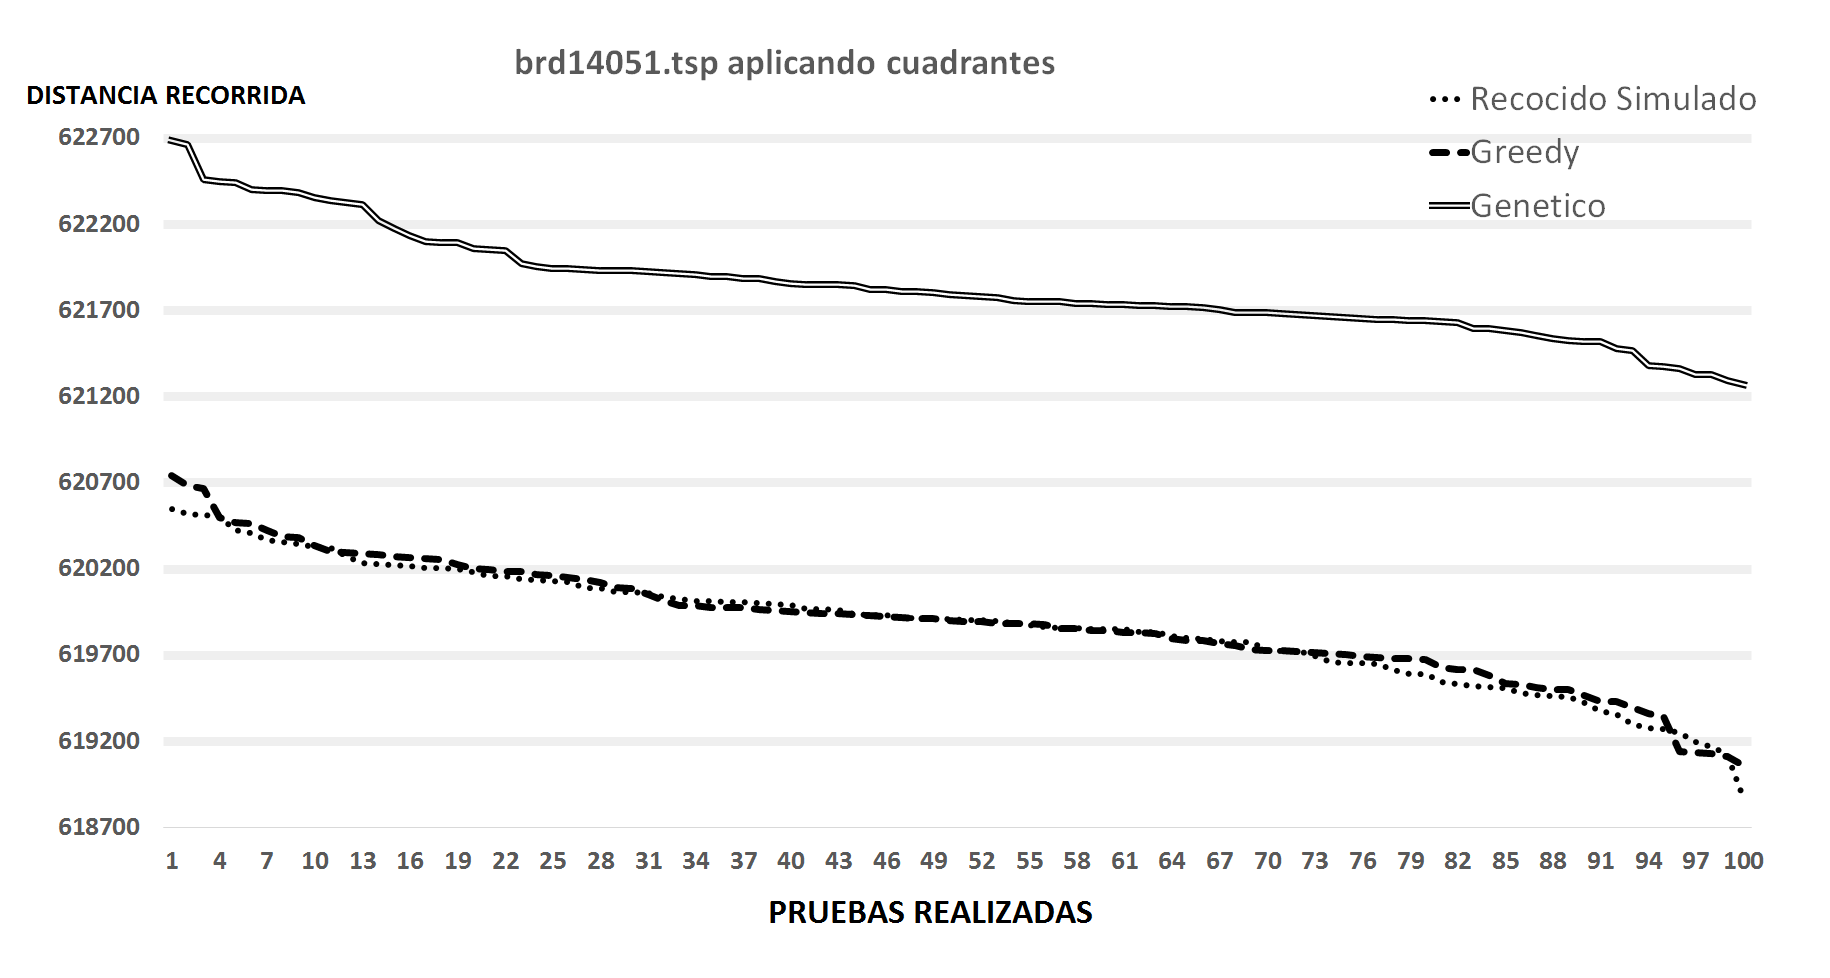
\includegraphics[width=0.9\textwidth]{PruebasResultados/Experimentos_Graficos_Con/brd14051.png}
        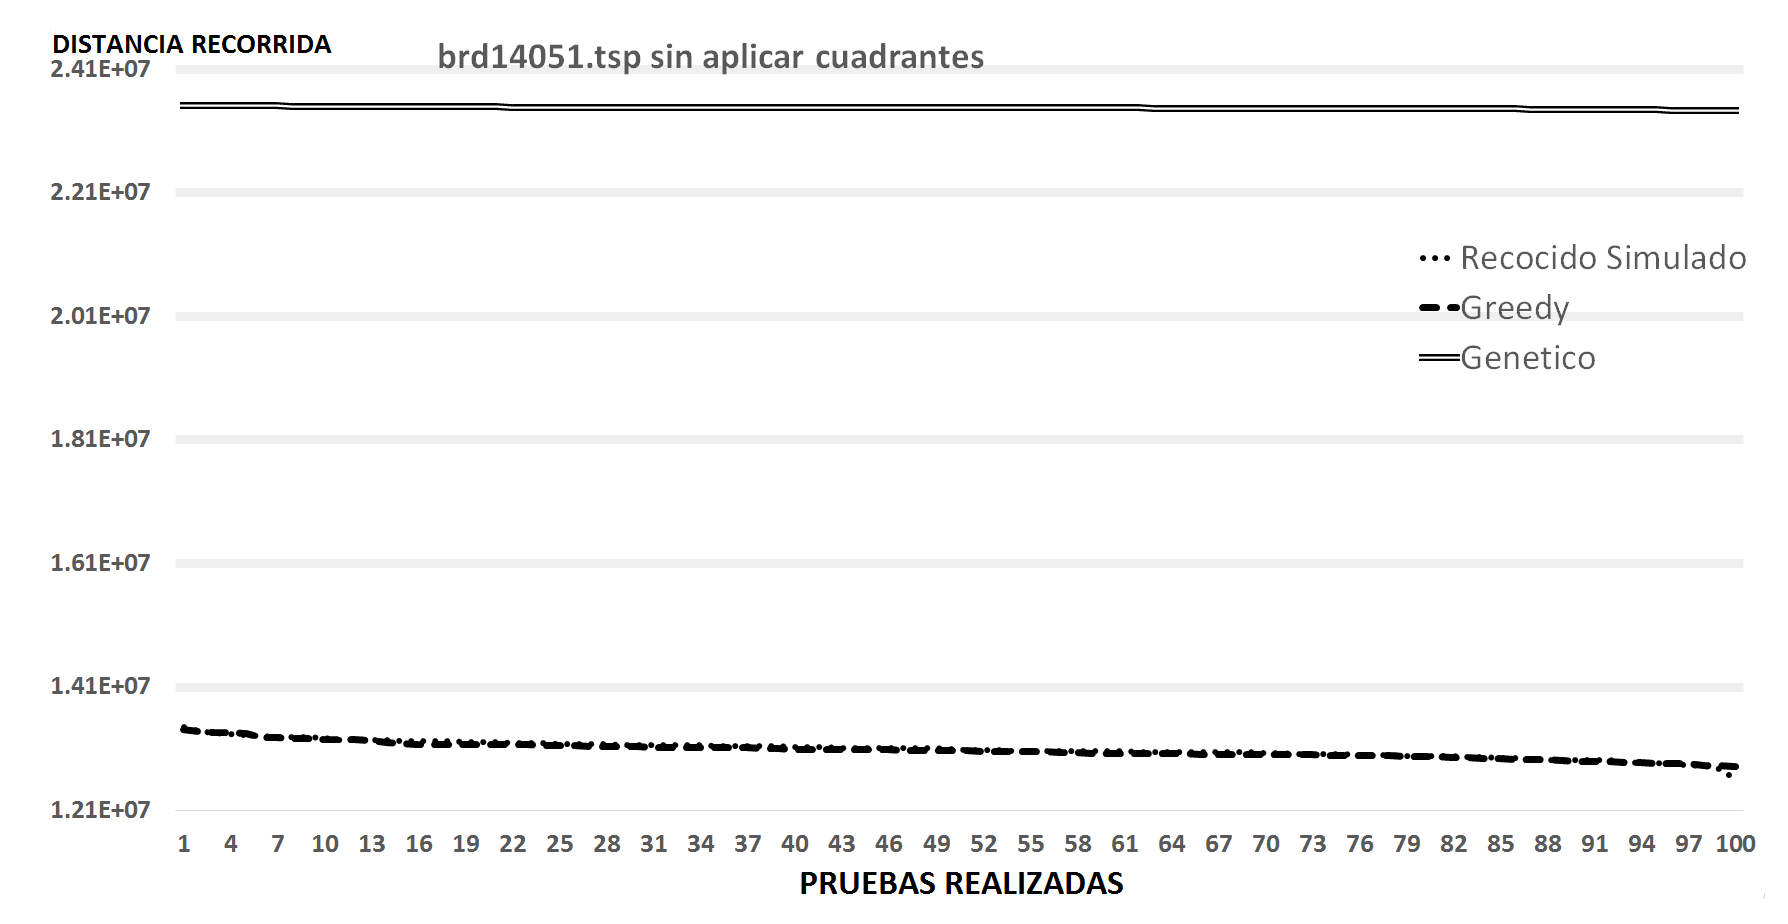
\includegraphics[width=0.9\textwidth]{PruebasResultados/Experimentos_Graficos_Sin/brd14051.png}
        \caption{Graficos brd14051.tsp con cuadrantes y sin cuadrantes}
        \label{fig:brd14051_grafica.png}
\end{figure}
\newpage

%d1655.TSP
\subsubsection{d1655.TSP}
\begin{table}[hbtp]
 \centering 
	\begin{tabular}{ | l   l | r | r | r |   }
         \hline\multicolumn{5}{|c|}{ \rowcolor[gray]{0.8}d1655.tsp    } \\\hline
         \multicolumn{2}{|l|}{Resultado Original :83605}  & Promedio & Mejor & Peor \\ \hline
                        & Recocido  & 82500.78 & 82098 & 82881  \\ 
         Con cuadrantes & Greedy    & 82489.63 & 82014 & 82839  \\ 
                        & Genetico  & 82244 & 81996 & 82447  \\ \hline
                        & Recocido  & 235605.87 & 222473 & 243750   \\ 
         Sin cuadrantes & Greedy    & 236306.2 & 226740 & 246172   \\ 
                        & Genetico  & 264556.11 & 262348 & 266415   \\ \hline
    \end{tabular}
    \caption{Experimento con la prueba d1655.tsp}
    \label{table:EXP_d1655.tsp}
\end{table}
\begin{figure}[hbtp]
    \centering
        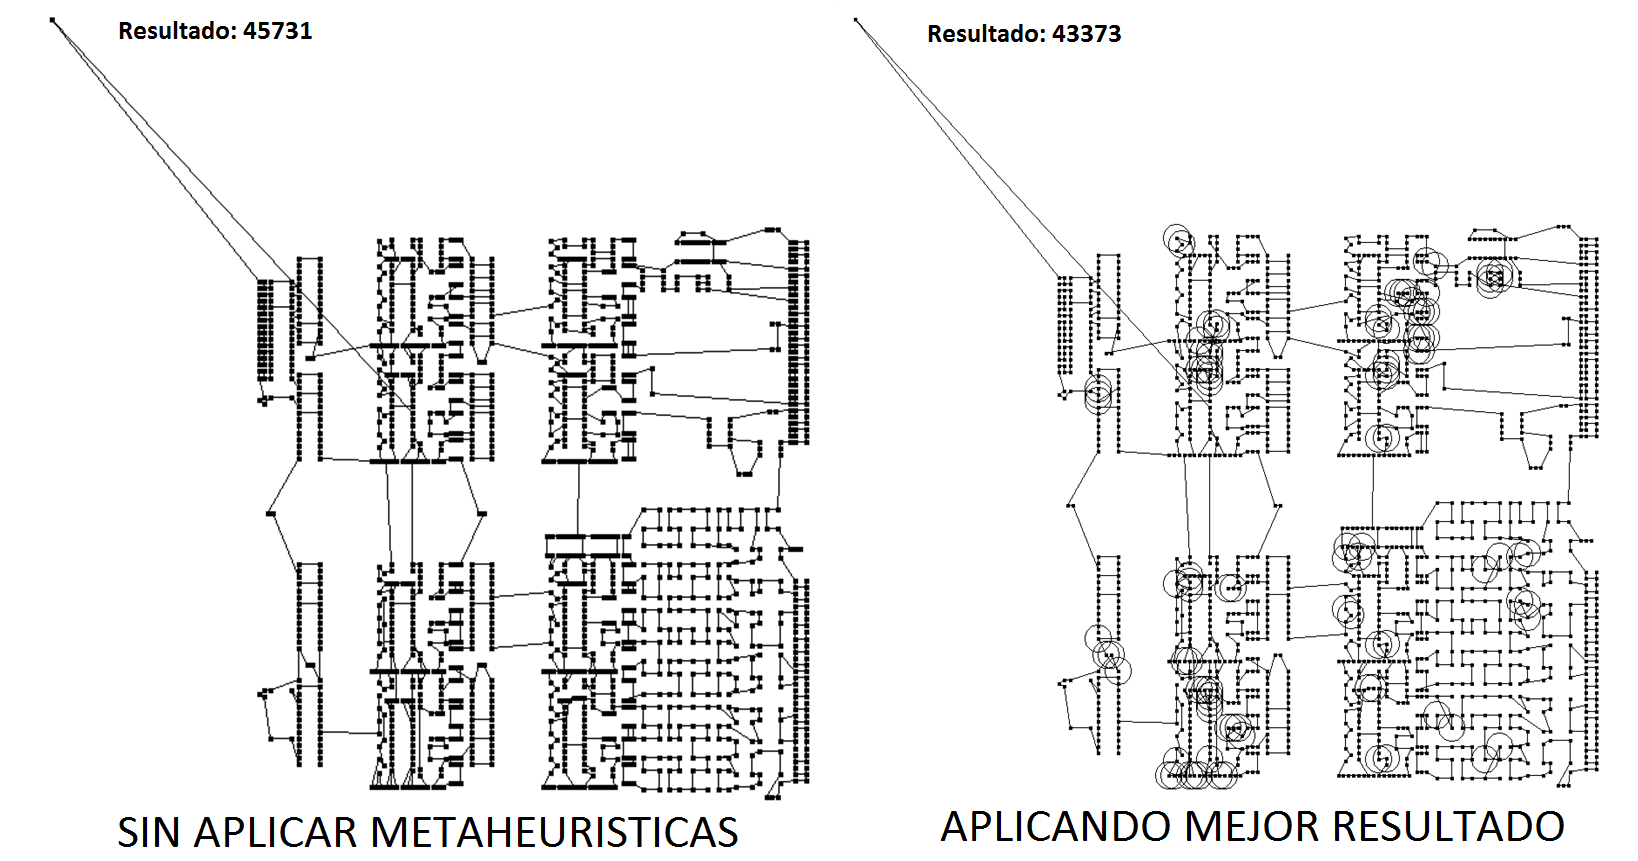
\includegraphics[width=1\textwidth]{PruebasResultados/Experimentos_Comparativas/d1655.png}
        \caption{Comparativa d1655.tsp}
        \label{fig:d1655_comparativa.png}
\end{figure}
 \begin{figure}[hbtp]
    \centering
        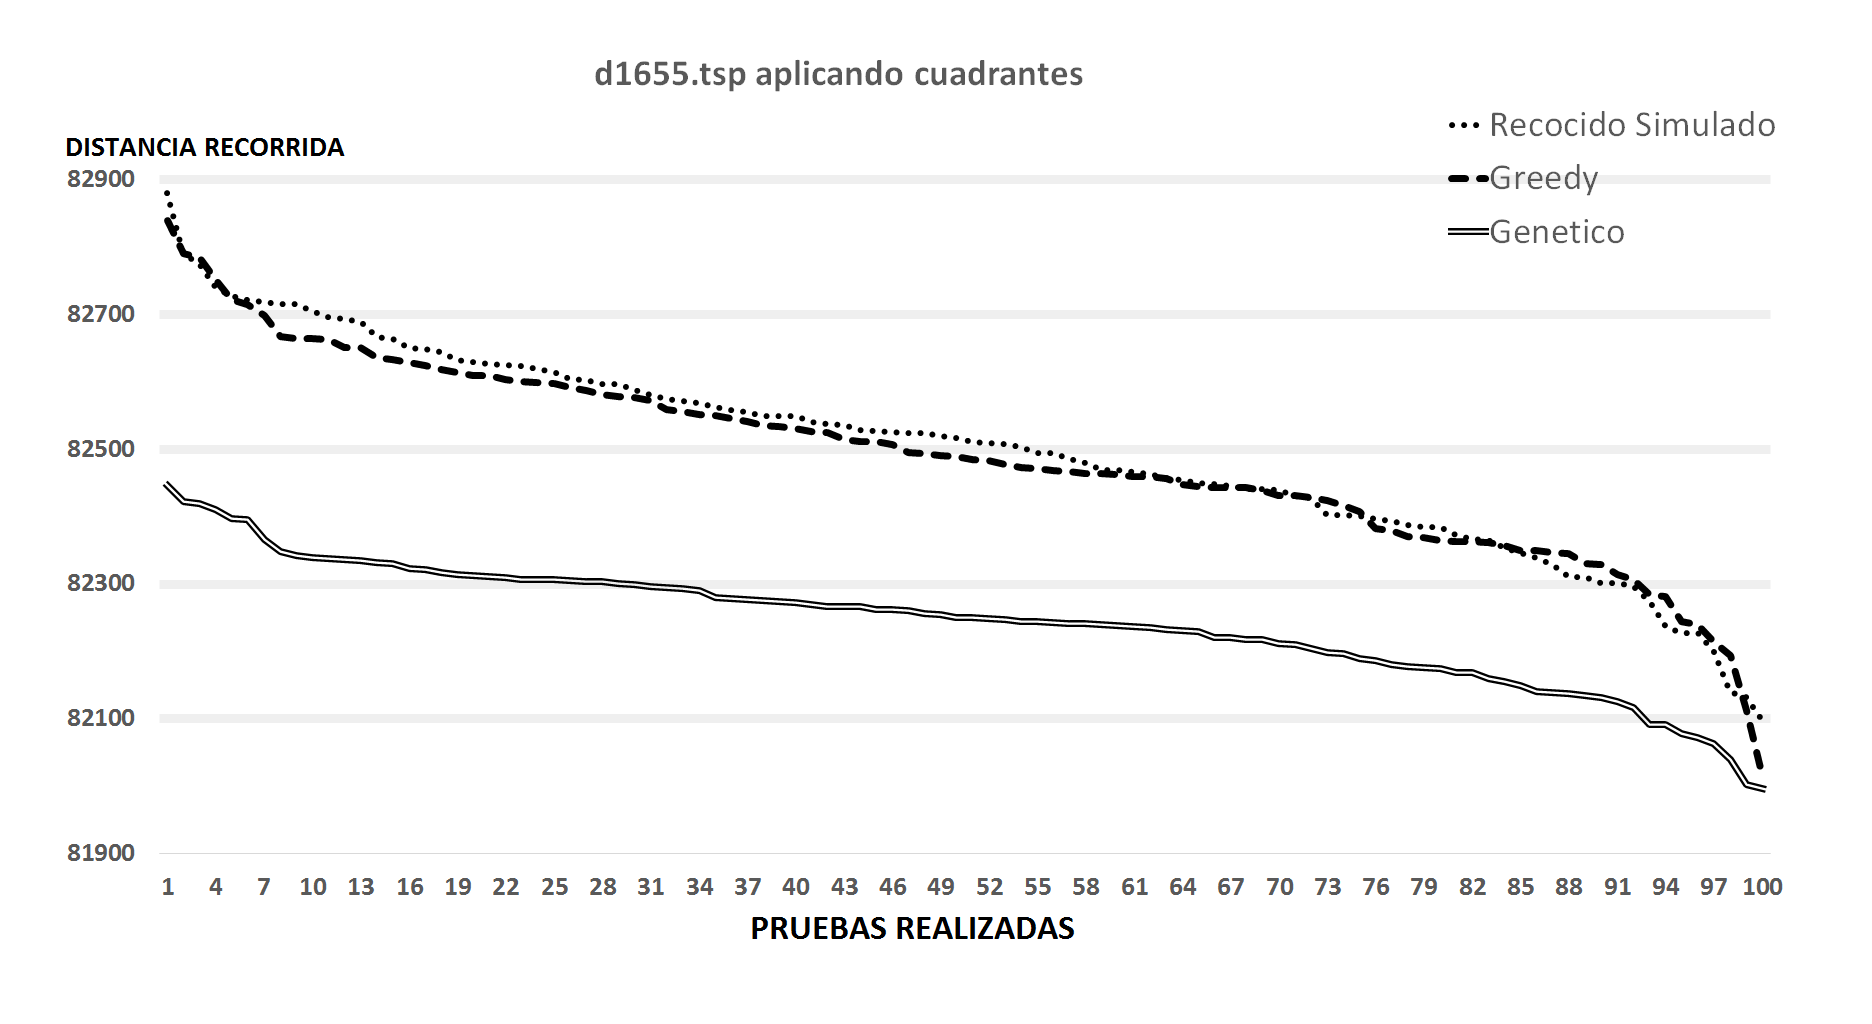
\includegraphics[width=0.9\textwidth]{PruebasResultados/Experimentos_Graficos_Con/d1655.png}
        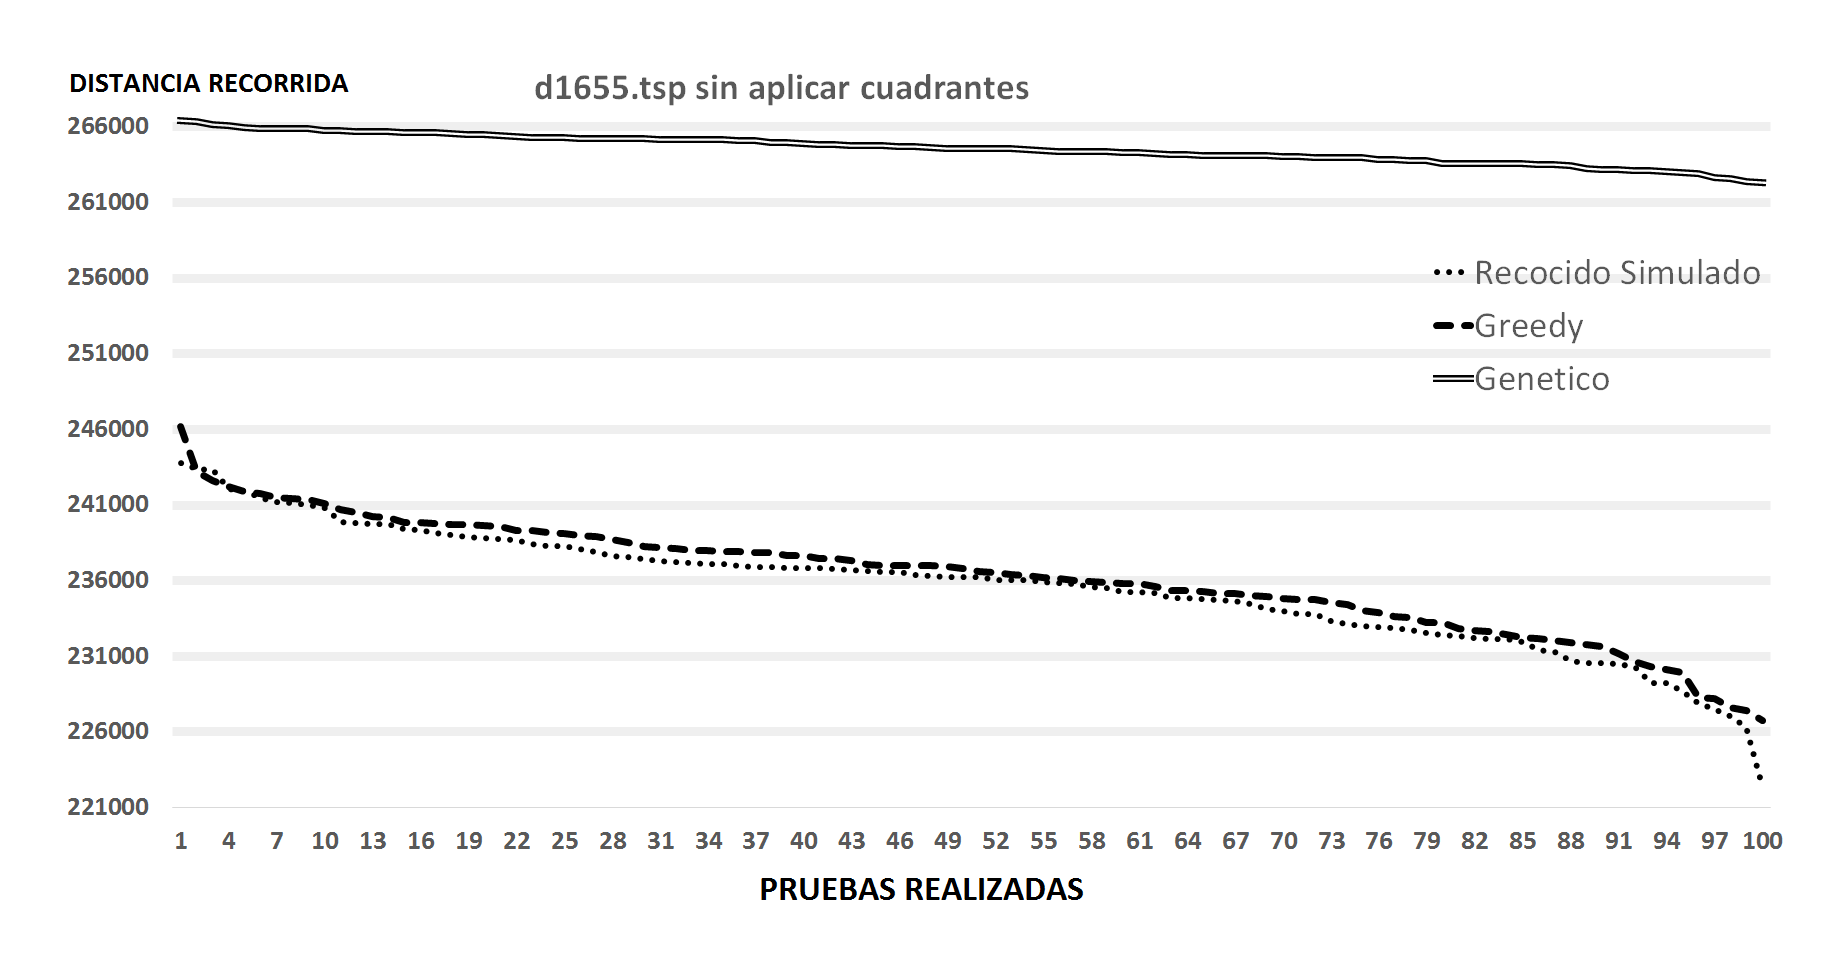
\includegraphics[width=0.9\textwidth]{PruebasResultados/Experimentos_Graficos_Sin/d1655.png}
        \caption{Graficos d1655.tsp con cuadrantes y sin cuadrantes}
        \label{fig:d1655_grafica.png}
\end{figure}
\newpage

%pcb3038.TSP
\subsubsection{pcb3038.TSP}
\begin{table}[hbtp]
 \centering 
	\begin{tabular}{ | l   l | r | r | r |   }
         \hline\multicolumn{5}{|c|}{ \rowcolor[gray]{0.8}pcb3038.tsp} \\\hline
        \multicolumn{2}{|l|}{Resultado Original :179474}  & Promedio & Mejor & Peor \\ \hline
                        & Recocido  & 176904.37 & 176488 & 177468  \\ 
         Con cuadrantes & Greedy    & 176903.86 & 176282 & 177403  \\ 
                        & Genetico  & 176989.64 & 176391 & 177957  \\ \hline
                        & Recocido  & 389970.63 & 384530 & 396772   \\ 
         Sin cuadrantes & Greedy    & 390708.99 & 382955 & 398492   \\ 
                        & Genetico  & 425459.53 & 422981 & 427722   \\ \hline
    \end{tabular}
    \caption{Experimento con la prueba pcb3038.tsp}
    \label{table:EXP_pcb3038.tsp}
\end{table}
\begin{figure}[hbtp]
    \centering
        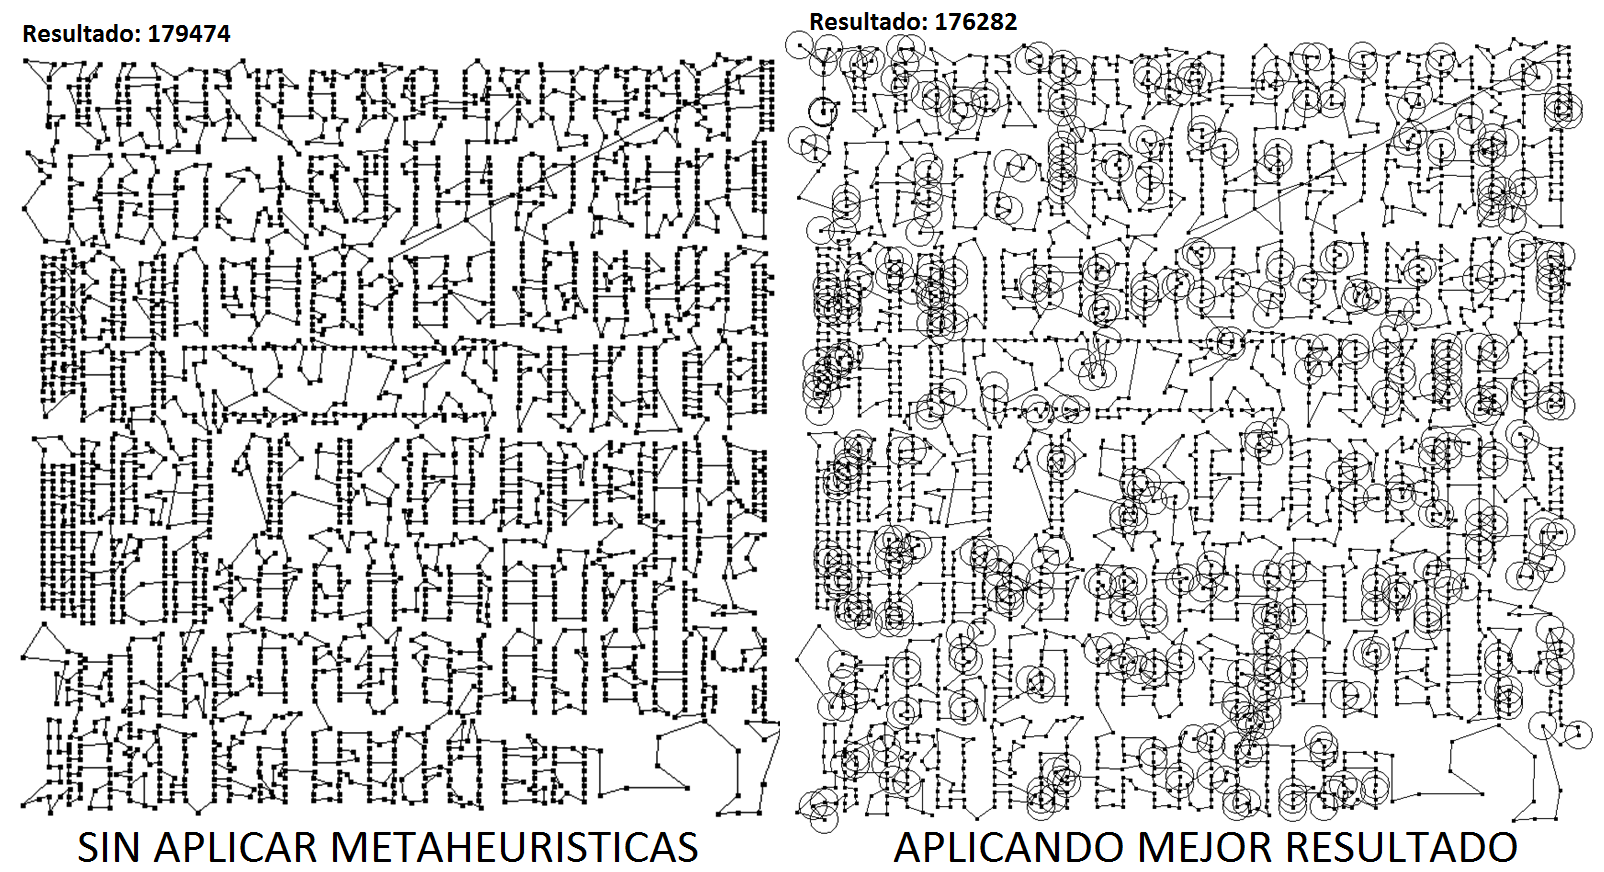
\includegraphics[width=1\textwidth]{PruebasResultados/Experimentos_Comparativas/pcb3038.png}
        \caption{Comparativa pcb3038.tsp}
        \label{fig:pcb3038_comparativa.png}
\end{figure}
 \begin{figure}[hbtp]
    \centering
        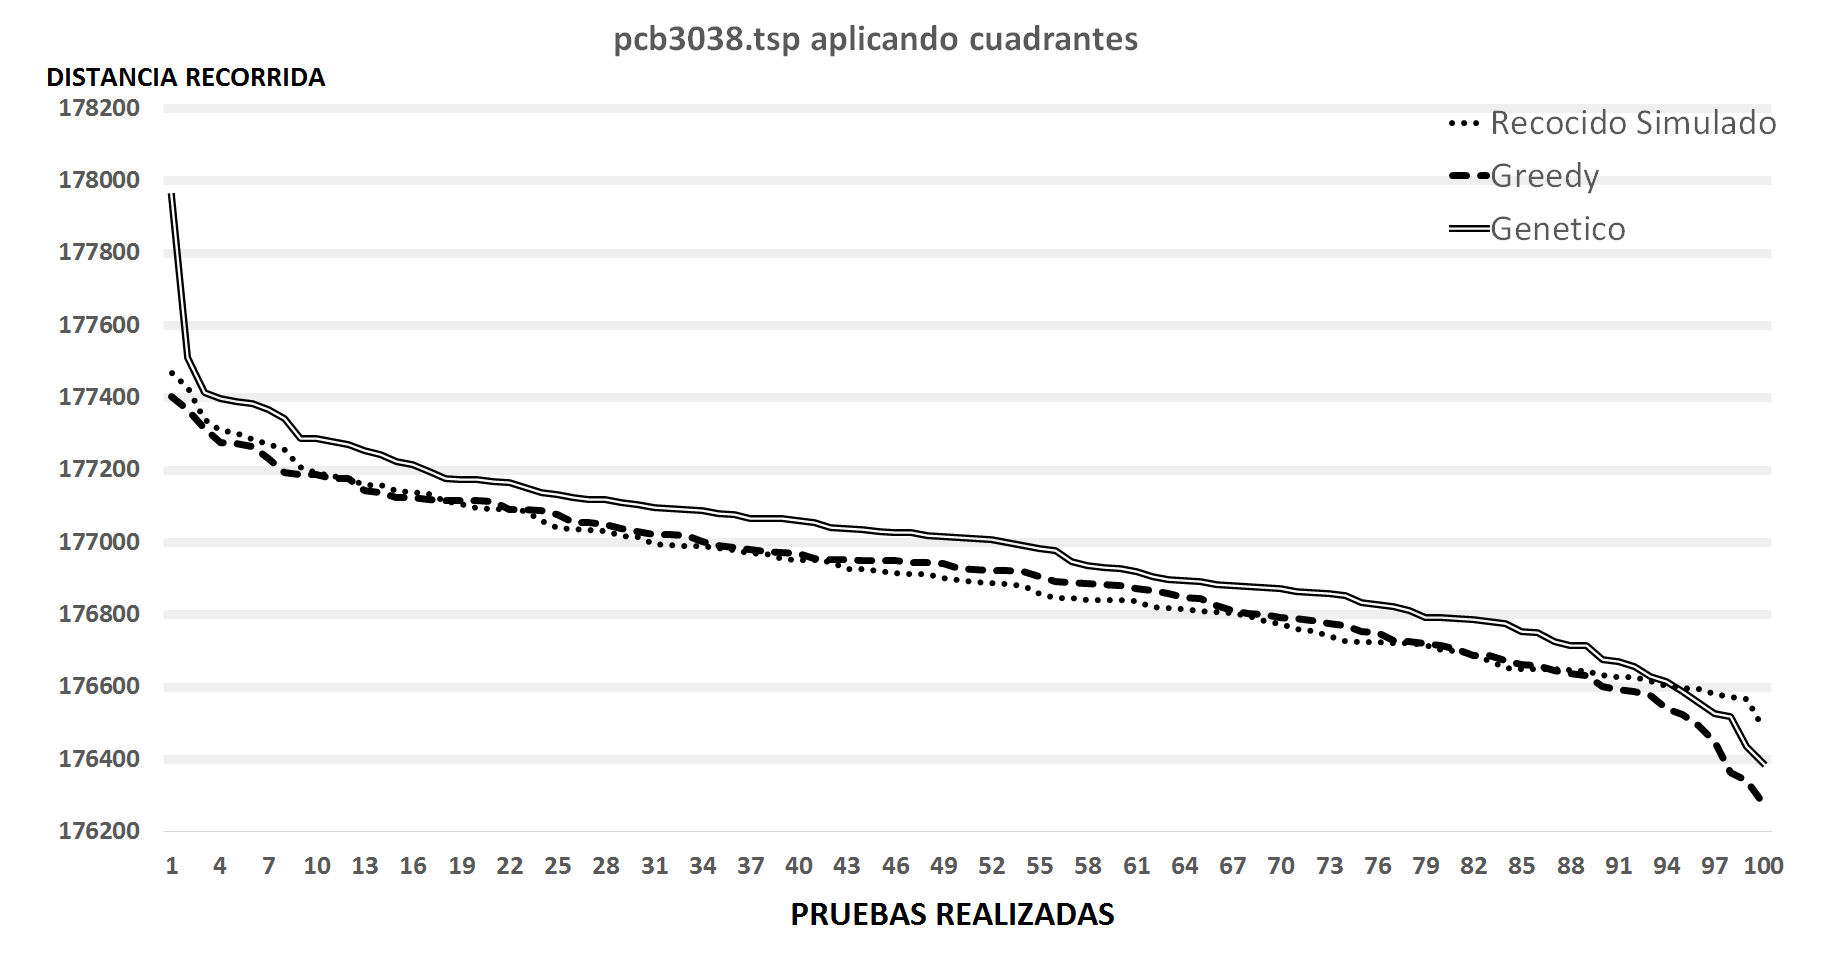
\includegraphics[width=0.9\textwidth]{PruebasResultados/Experimentos_Graficos_Con/pcb3038.png}
        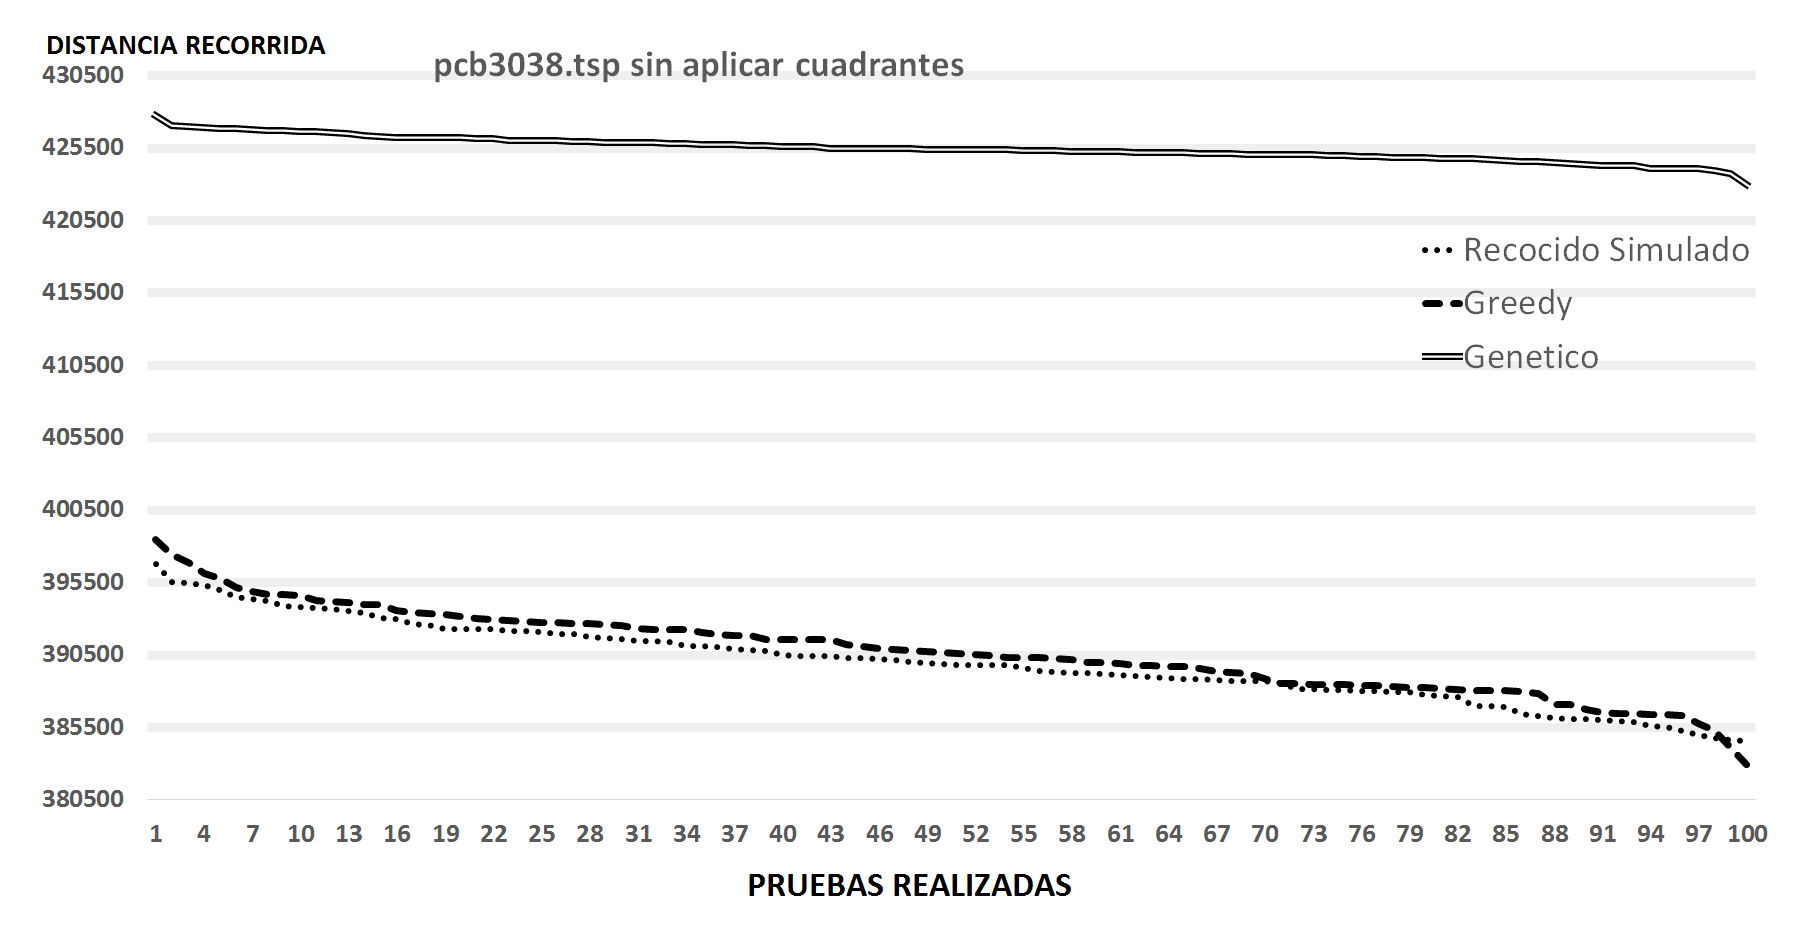
\includegraphics[width=0.9\textwidth]{PruebasResultados/Experimentos_Graficos_Sin/pcb3038.png}
        \caption{Graficos pcb3038.tsp con cuadrantes y sin cuadrantes}
        \label{fig:pcb3038_grafica.png}
\end{figure}
\newpage

%rl5934.TSP
\subsubsection{rl5934.TSP}
\begin{table}[hbtp]
 \centering 
	\begin{tabular}{ | l   l | r | r | r |   }
         \hline\multicolumn{5}{|c|}{ \rowcolor[gray]{0.8}rl5934.tsp} \\\hline
         \multicolumn{2}{|l|}{Resultado Original :785540}  & Promedio & Mejor & Peor \\ \hline
                        & Recocido  & 774838.4 & 772530 & 777479  \\ 
         Con cuadrantes & Greedy    & 774761.73 & 772083 & 778205  \\ 
                        & Genetico  & 777549.96 & 776338 & 779039  \\ \hline
                        & Recocido  & 9349554.00 & 9184381 & 9492444   \\ 
         Sin cuadrantes & Greedy    & 9348025.21 & 9240374 & 9497166   \\ 
                        & Genetico  & 10249756.12 & 10213188 & 10282877   \\ \hline
    \end{tabular}
    \caption{Experimento con la prueba rl5934.tsp}
    \label{table:EXP_rl5934.tsp}
\end{table}
\begin{figure}[hbtp]
    \centering
        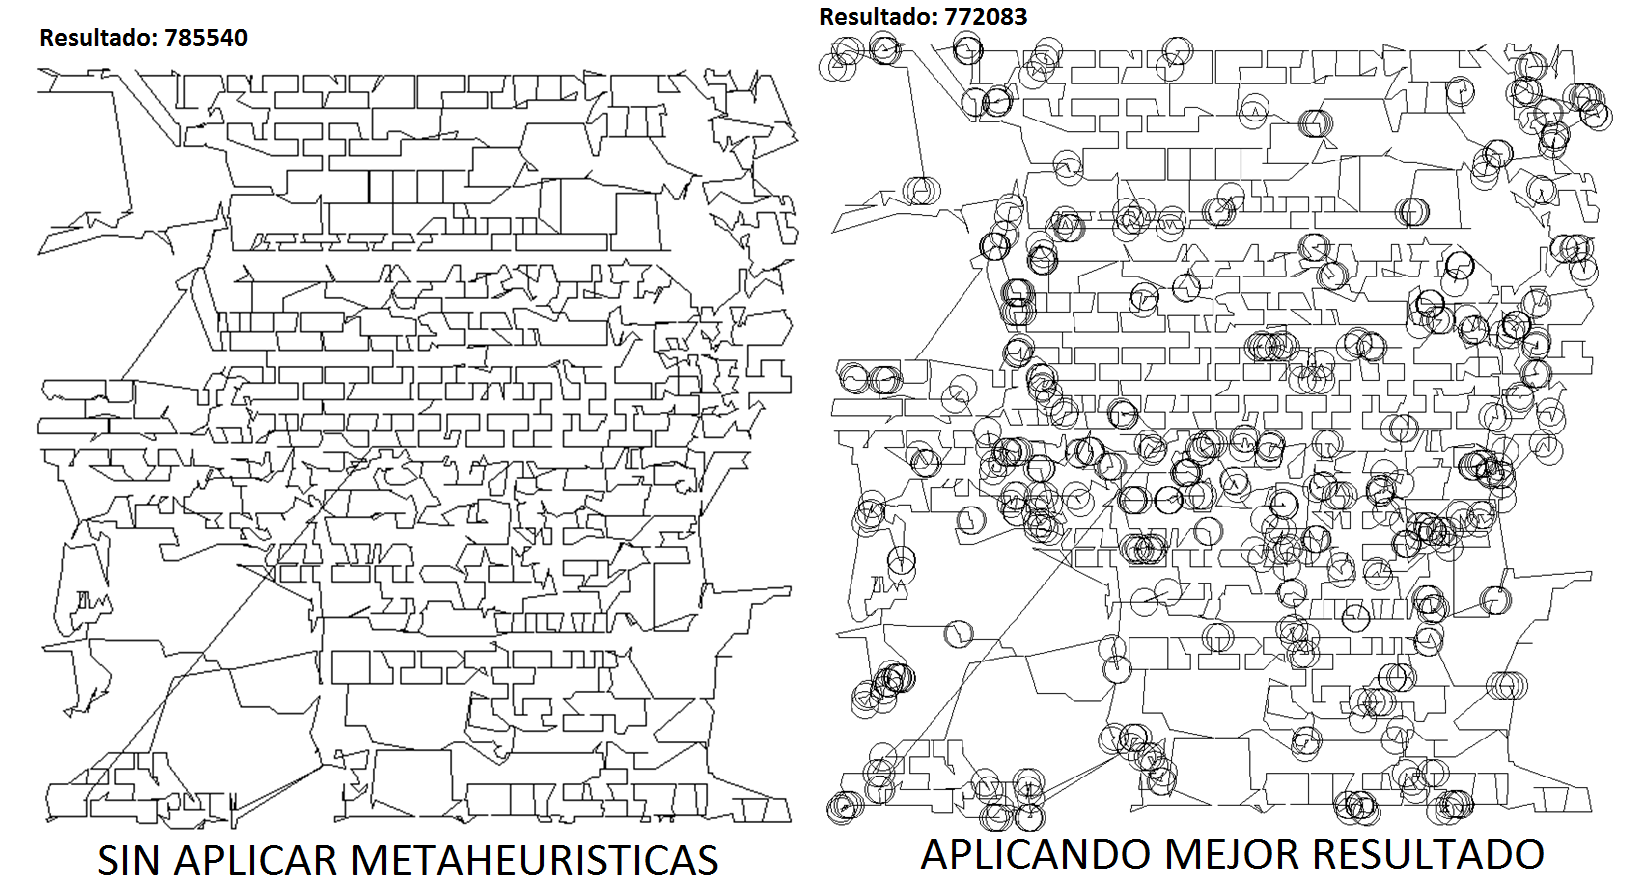
\includegraphics[width=1\textwidth]{PruebasResultados/Experimentos_Comparativas/rl5934.png}
        \caption{Comparativa rl5934.tsp}
        \label{fig:rl5934_comparativa.png}
\end{figure}
 \begin{figure}[hbtp]
    \centering
        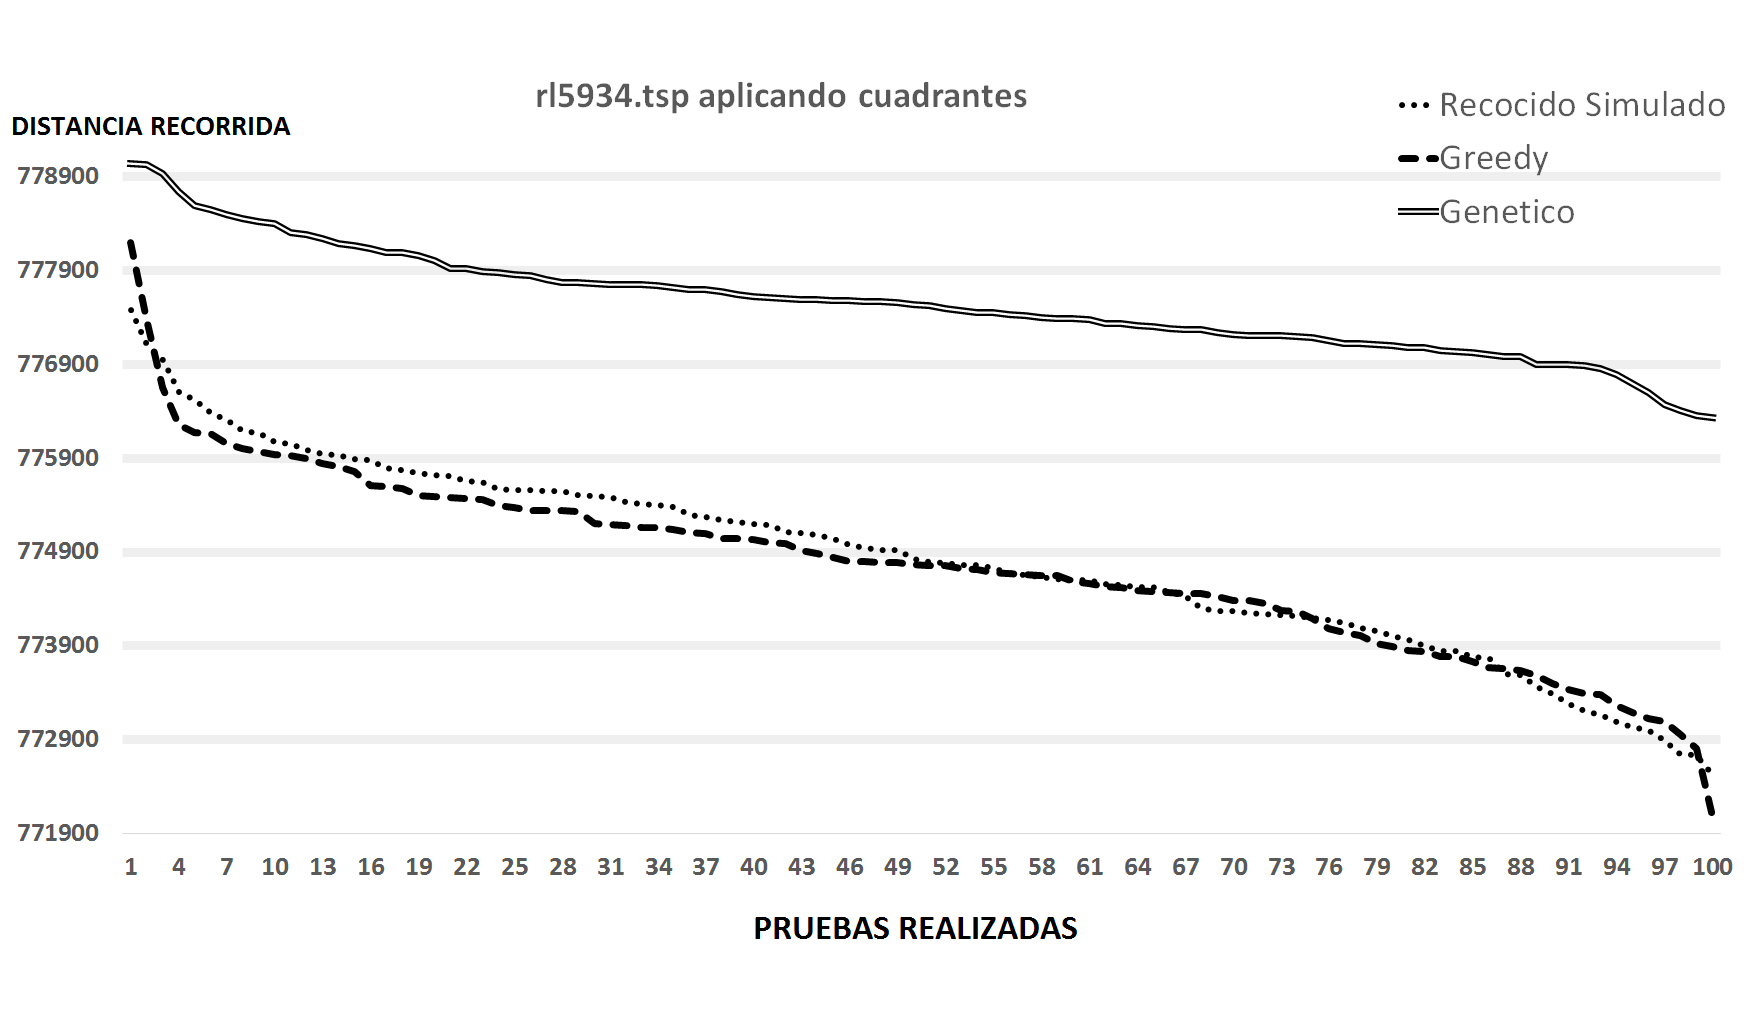
\includegraphics[width=0.9\textwidth]{PruebasResultados/Experimentos_Graficos_Con/rl5934.png}
        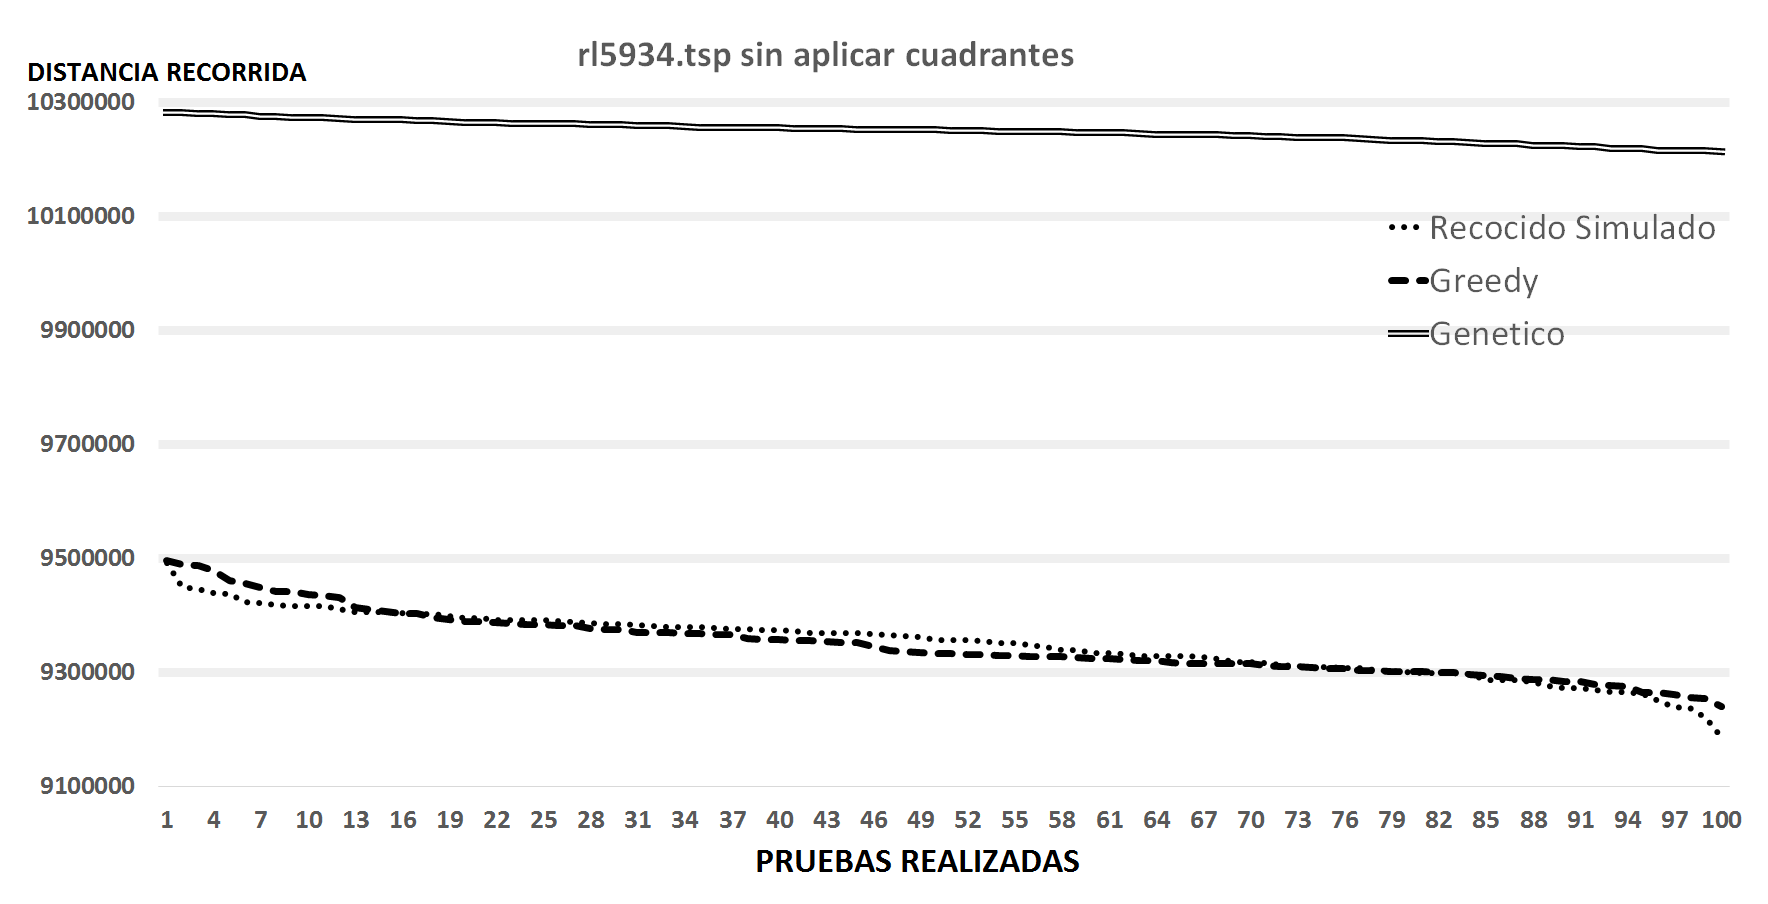
\includegraphics[width=0.9\textwidth]{PruebasResultados/Experimentos_Graficos_Sin/rl5934.png}
        \caption{Graficos rl5934.tsp con cuadrantes y sin cuadrantes}
        \label{fig:rl5934_grafica.png}
\end{figure}
\newpage

%vm1084.TSP
\subsubsection{vm1084.TSP}
\begin{table}[hbtp]
 \centering 
	\begin{tabular}{ | l   l | r | r | r |   }
         \hline\multicolumn{5}{|c|}{ \rowcolor[gray]{0.8}vm1084.tsp} \\\hline
         \multicolumn{2}{|l|}{Resultado Original :344972}  & Promedio & Mejor & Peor \\ \hline
                        & Recocido  & 334821.39 & 330999 & 338557  \\ 
         Con cuadrantes & Greedy    & 335133.04 & 331589 & 339023  \\ 
                        & Genetico  & 331384.21 & 329200 & 333749  \\ \hline
                        & Recocido  & 3224207.18 & 3064309 & 3380496   \\ 
         Sin cuadrantes & Greedy    & 3214476.72 & 3063644 & 3363287   \\ 
                        & Genetico  & 4772212.30 & 4671155 & 4850260   \\ \hline
    \end{tabular}
    \caption{Experimento con la prueba vm1084.tsp}
    \label{table:EXP_vm1084.tsp}
\end{table}
\begin{figure}[hbtp]
    \centering
        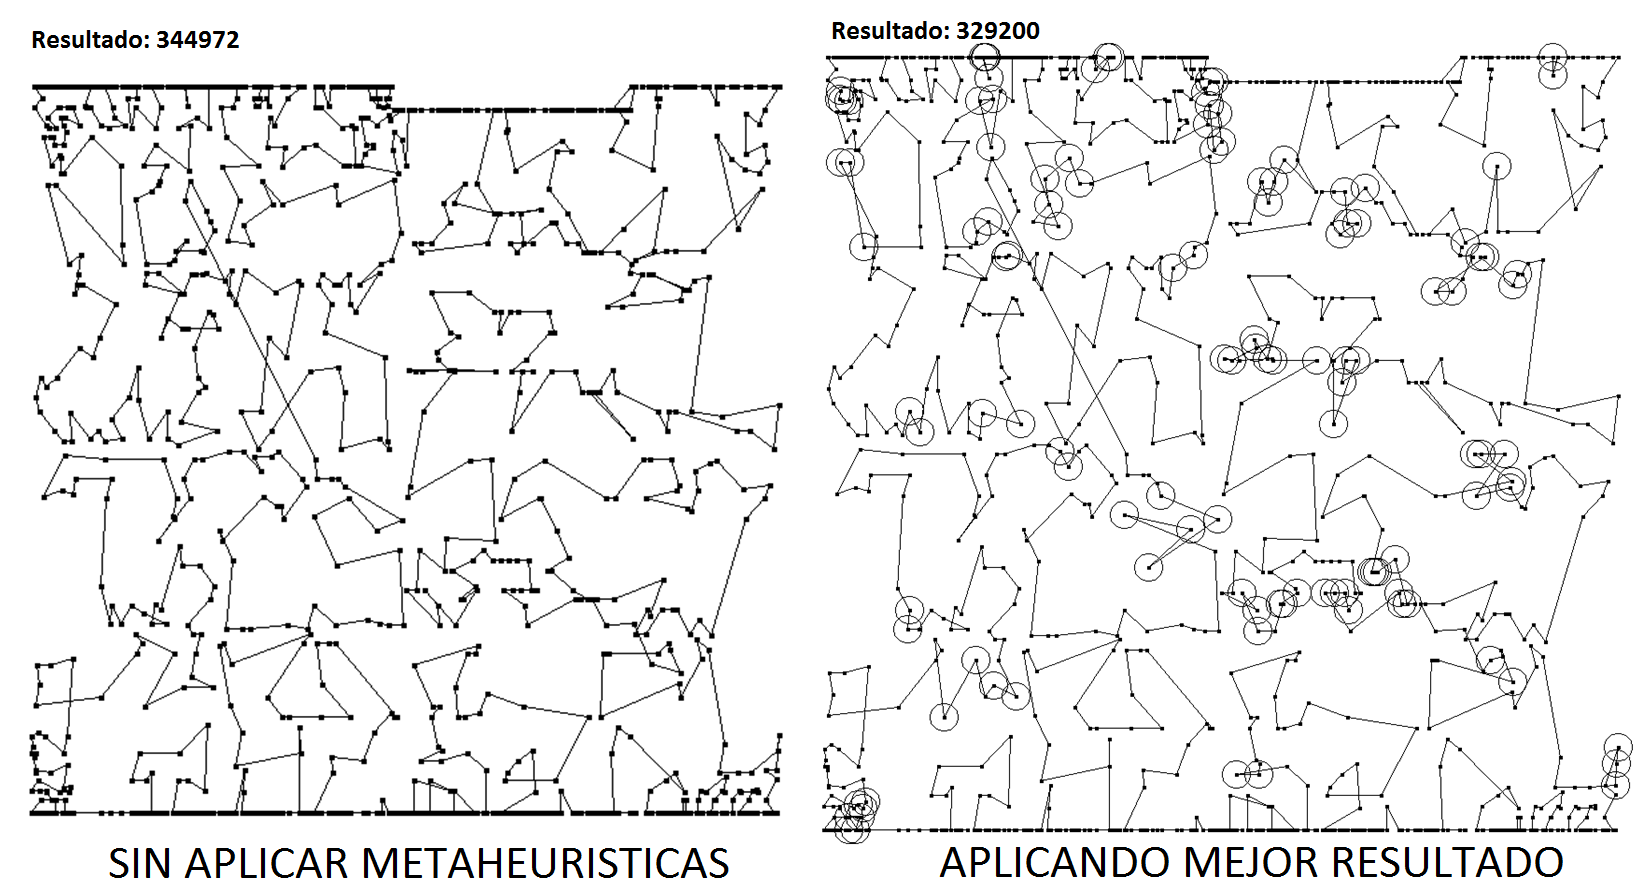
\includegraphics[width=1\textwidth]{PruebasResultados/Experimentos_Comparativas/vm1084.png}
        \caption{Comparativa vm1084.tsp}
        \label{fig:vm1084_comparativa.png}
\end{figure}
 \begin{figure}[hbtp]
    \centering
        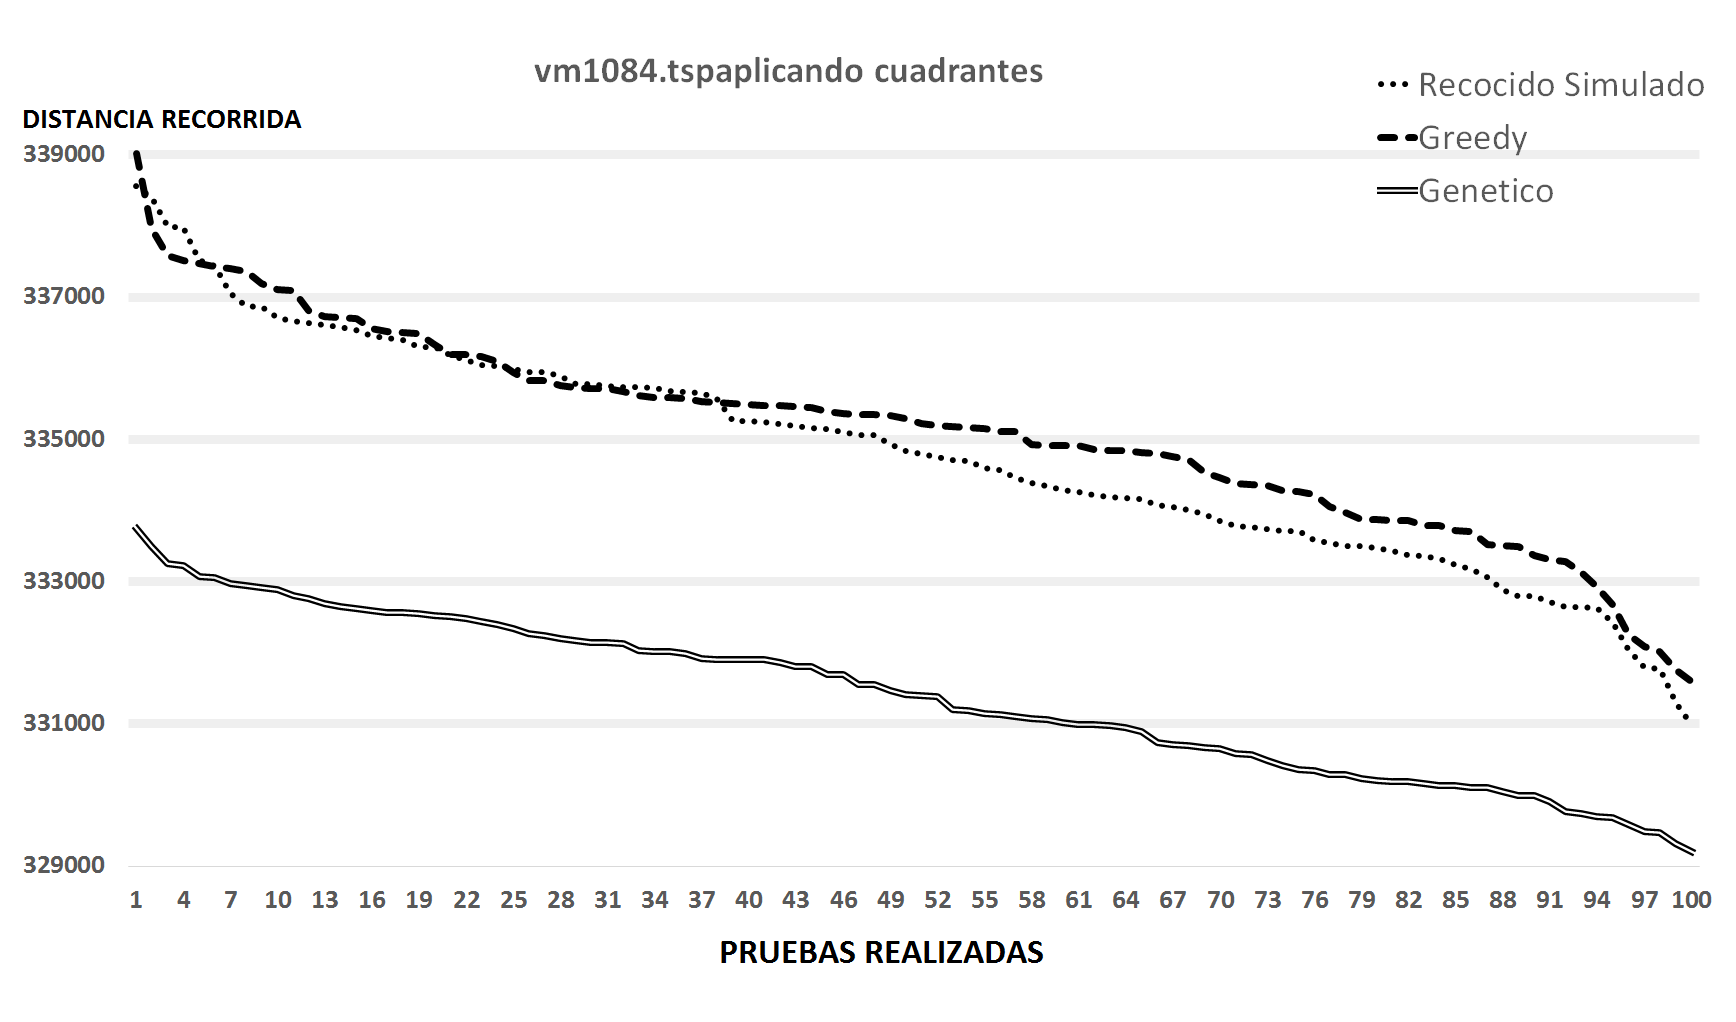
\includegraphics[width=0.9\textwidth]{PruebasResultados/Experimentos_Graficos_Con/vm1084.png}
        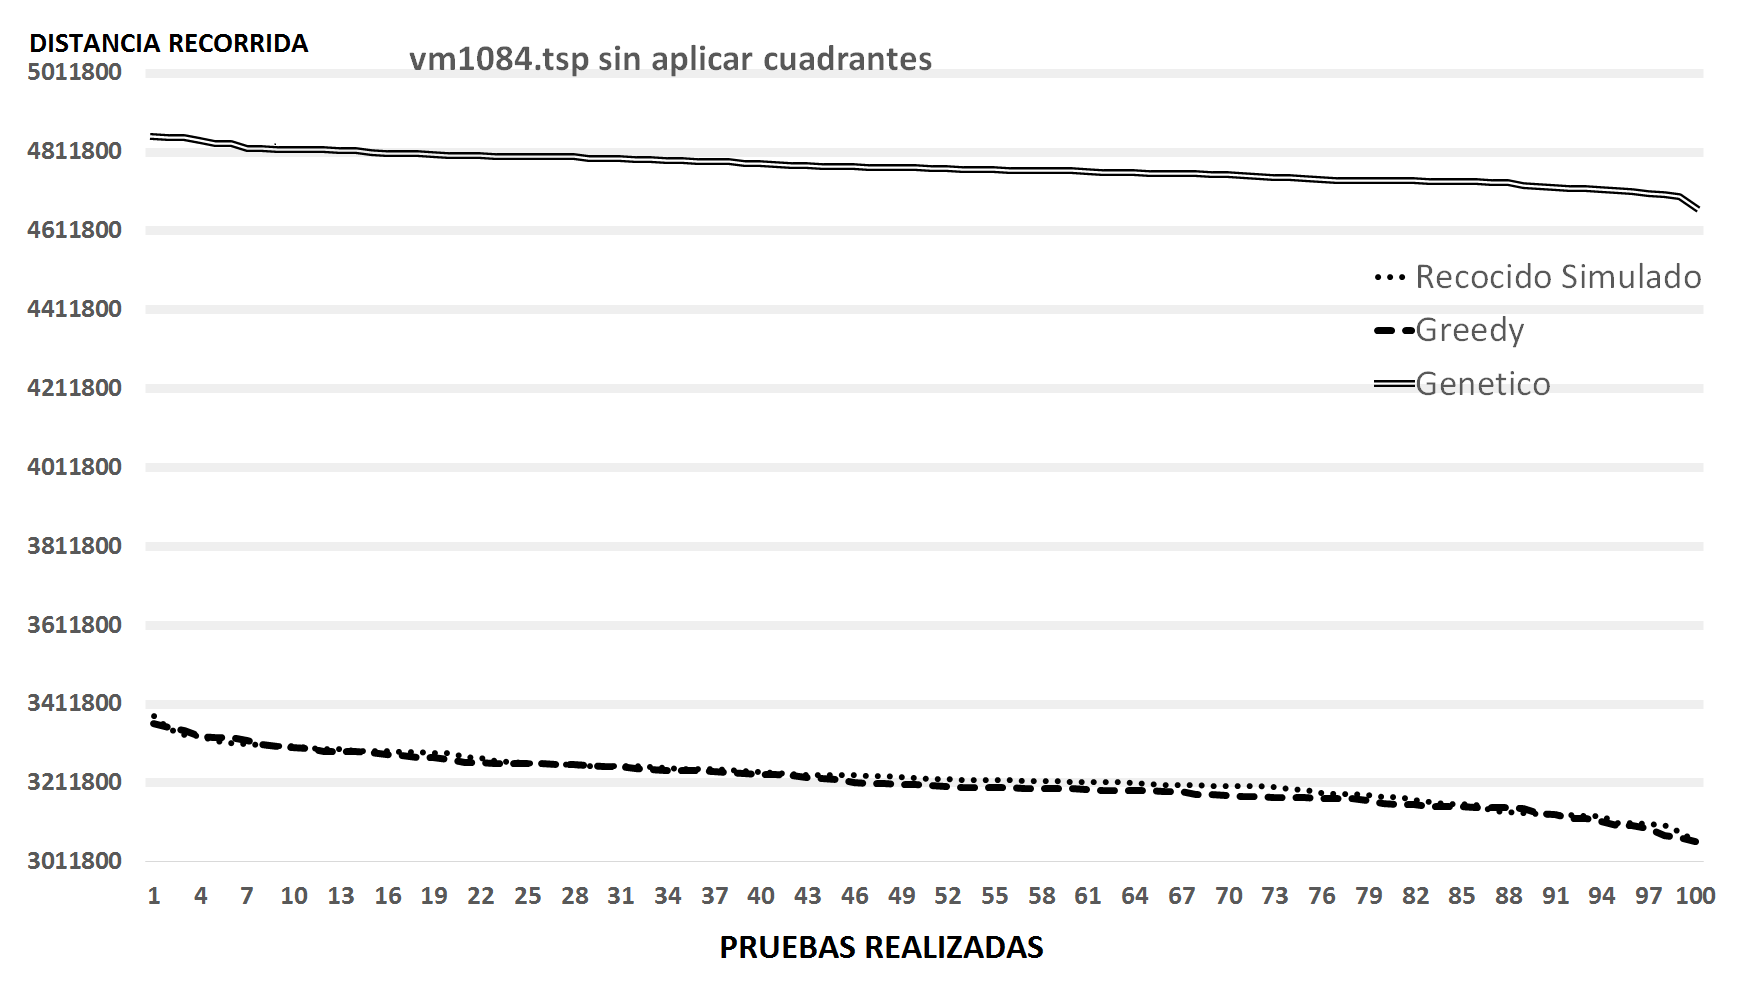
\includegraphics[width=0.9\textwidth]{PruebasResultados/Experimentos_Graficos_Sin/vm1084.png}
        \caption{Graficos vm1084.tsp con cuadrantes y sin cuadrantes}
        \label{fig:vm1084_grafica.png}
\end{figure}
\newpage



 %\begin{figure}[hbtp]
    %\centering
       
     %   \caption{Grafico a280.tsp sin cuadrantes}
      %  \label{fig:a280_comparativa.png}
%\end{figure}